% Options for packages loaded elsewhere
\PassOptionsToPackage{unicode}{hyperref}
\PassOptionsToPackage{hyphens}{url}
\documentclass[
  12pt,
]{article}
\usepackage{xcolor}
\usepackage[margin=1in]{geometry}
\usepackage{amsmath,amssymb}
\setcounter{secnumdepth}{5}
\usepackage{iftex}
\ifPDFTeX
  \usepackage[T1]{fontenc}
  \usepackage[utf8]{inputenc}
  \usepackage{textcomp} % provide euro and other symbols
\else % if luatex or xetex
  \usepackage{unicode-math} % this also loads fontspec
  \defaultfontfeatures{Scale=MatchLowercase}
  \defaultfontfeatures[\rmfamily]{Ligatures=TeX,Scale=1}
\fi
\usepackage{lmodern}
\ifPDFTeX\else
  % xetex/luatex font selection
\fi
% Use upquote if available, for straight quotes in verbatim environments
\IfFileExists{upquote.sty}{\usepackage{upquote}}{}
\IfFileExists{microtype.sty}{% use microtype if available
  \usepackage[]{microtype}
  \UseMicrotypeSet[protrusion]{basicmath} % disable protrusion for tt fonts
}{}
\makeatletter
\@ifundefined{KOMAClassName}{% if non-KOMA class
  \IfFileExists{parskip.sty}{%
    \usepackage{parskip}
  }{% else
    \setlength{\parindent}{0pt}
    \setlength{\parskip}{6pt plus 2pt minus 1pt}}
}{% if KOMA class
  \KOMAoptions{parskip=half}}
\makeatother
\usepackage{graphicx}
\makeatletter
\newsavebox\pandoc@box
\newcommand*\pandocbounded[1]{% scales image to fit in text height/width
  \sbox\pandoc@box{#1}%
  \Gscale@div\@tempa{\textheight}{\dimexpr\ht\pandoc@box+\dp\pandoc@box\relax}%
  \Gscale@div\@tempb{\linewidth}{\wd\pandoc@box}%
  \ifdim\@tempb\p@<\@tempa\p@\let\@tempa\@tempb\fi% select the smaller of both
  \ifdim\@tempa\p@<\p@\scalebox{\@tempa}{\usebox\pandoc@box}%
  \else\usebox{\pandoc@box}%
  \fi%
}
% Set default figure placement to htbp
\def\fps@figure{htbp}
\makeatother
\setlength{\emergencystretch}{3em} % prevent overfull lines
\providecommand{\tightlist}{%
  \setlength{\itemsep}{0pt}\setlength{\parskip}{0pt}}
\usepackage{url}
%\usepackage{xurl}
\usepackage{setspace}
\singlespacing
%\onehalfspacing
%\doublespacing
\usepackage{lineno}
%\linenumbers
\usepackage[belowskip=0pt,aboveskip=0pt]{caption}
\usepackage{relsize}
\usepackage{float}
\usepackage{lscape}
\usepackage{longtable}
\usepackage{amsmath,rotating}
\usepackage[scanall]{psfrag}
\usepackage{bm}
\usepackage{caption,graphics}
\usepackage{graphicx}
\usepackage{sectsty}
\usepackage{color}
\usepackage{fancyhdr}
\usepackage{xspace}
\usepackage{textcomp}
\usepackage{upgreek}
\renewcommand\figurename{Fig.}
\captionsetup{labelsep=period, singlelinecheck=false}
\newcommand{\changesize}[1]{\fontsize{#1pt}{#1pt}\selectfont}
\renewcommand{\arraystretch}{1.5}
%\renewcommand\theadfont{}

\newcommand{\Fmsy}{\ensuremath{F_{\text{MSY}}}\xspace}
\newcommand{\Fspr}[1]{\ensuremath{F_{\text{{#1}\%}}}\xspace}
\usepackage{booktabs}
\usepackage{longtable}
\usepackage{array}
\usepackage{multirow}
\usepackage{wrapfig}
\usepackage{float}
\usepackage{colortbl}
\usepackage{pdflscape}
\usepackage{tabu}
\usepackage{threeparttable}
\usepackage{threeparttablex}
\usepackage[normalem]{ulem}
\usepackage{makecell}
\usepackage{xcolor}
\usepackage{bookmark}
\IfFileExists{xurl.sty}{\usepackage{xurl}}{} % add URL line breaks if available
\urlstyle{same}
\hypersetup{
  hidelinks,
  pdfcreator={LaTeX via pandoc}}

\title{An investigation of factors affecting inferences from and
reliability of state-space age-structured assessment models:\\
Supplementary Materials}
\author{}
\date{\vspace{-2.5em}}

\begin{document}
\maketitle

Timothy J. Miller: ORCID ID 0000-0003-1411-1206; corresponding author:
\href{mailto:timothy.j.miller@noaa.gov}{\nolinkurl{timothy.j.miller@noaa.gov}};
Northeast Fisheries Science Center, Woods Hole Laboratory, 166 Water
Street, Woods Hole, MA 02543 USA\\
\strut \\
Gregory L. Britten: ORCID ID 0000-0003-1391-9086; Biology Department,
Woods Hole Oceanographic Institution, 266 Woods Hole Rd. Woods Hole, MA,
USA\\
\strut \\
Elizabeth N. Brooks: ORCID ID 0000-0002-9142-4372; Northeast Fisheries
Science Center, Woods Hole Laboratory, 166 Water Street, Woods Hole, MA
02543 USA\\
\strut \\
Gavin Fay: ORCID ID 0000-0003-0425-9952; Department of Fisheries
Oceanography, School for Marine Science and Technology, University of
Massachusetts Dartmouth, 836 S Rodney French Boulevard, New Bedford, MA
02740, USA\\
\strut \\
Alexander C. Hansell: ORCID ID 0000-0001-7827-1749; Northeast Fisheries
Science Center, Woods Hole Laboratory, 166 Water Street, Woods Hole, MA
02543 USA\\
\strut \\
Christopher M. Legault: ORCID ID 0000-0002-0328-1376; Northeast
Fisheries Science Center, Woods Hole Laboratory, 166 Water Street, Woods
Hole, MA 02543 USA\\
\strut \\
Chengxue Li: ORCID ID 0000-0001-7518-7234; Northeast Fisheries Science
Center, Woods Hole Laboratory, 166 Water Street, Woods Hole, MA 02543
USA; Current Address: Stony Brook University, Stony Brook, NY 11794
USA\\
\strut \\
Brandon Muffley: ORCID ID 0009-0005-8681-0489; Mid-Atlantic Fishery
Management Council, 800 North State Street, Suite 201, Dover, DE 19901
USA\\
\strut \\
Brian C. Stock: ORCID ID 0000-0002-2393-6747; Institute of Marine
Research, Nye Flødevigveien 20, 4817 His, Norway\\
\strut \\
John Wiedenmann: ORCID ID 0000-0001-7622-9053; Department of Ecology,
Evolution, and Natural Resources, Rutgers University, 14 College Farm Rd
W, New Brunswick, NJ 08901 USA\\

\pagebreak

\setcounter{figure}{0}
\renewcommand\thefigure{S\arabic{figure}}

\setcounter{table}{0}
\renewcommand\thetable{S\arabic{table}}

\pagebreak

\pagebreak

\section*{Referenced Figures}\label{referenced-figures}
\addcontentsline{toc}{section}{Referenced Figures}

\begin{figure}[!ht]
\begin{center}

\includegraphics[width = \textwidth]{om_input_plots_figure}
\end{center}
\caption{The proportion mature at age, weight at age, fleet and index selectivity at age, and Beverton-Holt SRR assumed for the population in all OMs. For OMs with random effects on fleet selectivity, this represents the selectivity at the mean of the random effects.}\label{om_inputs_fig}
\end{figure}

\begin{landscape}
\begin{figure}
\begin{center}
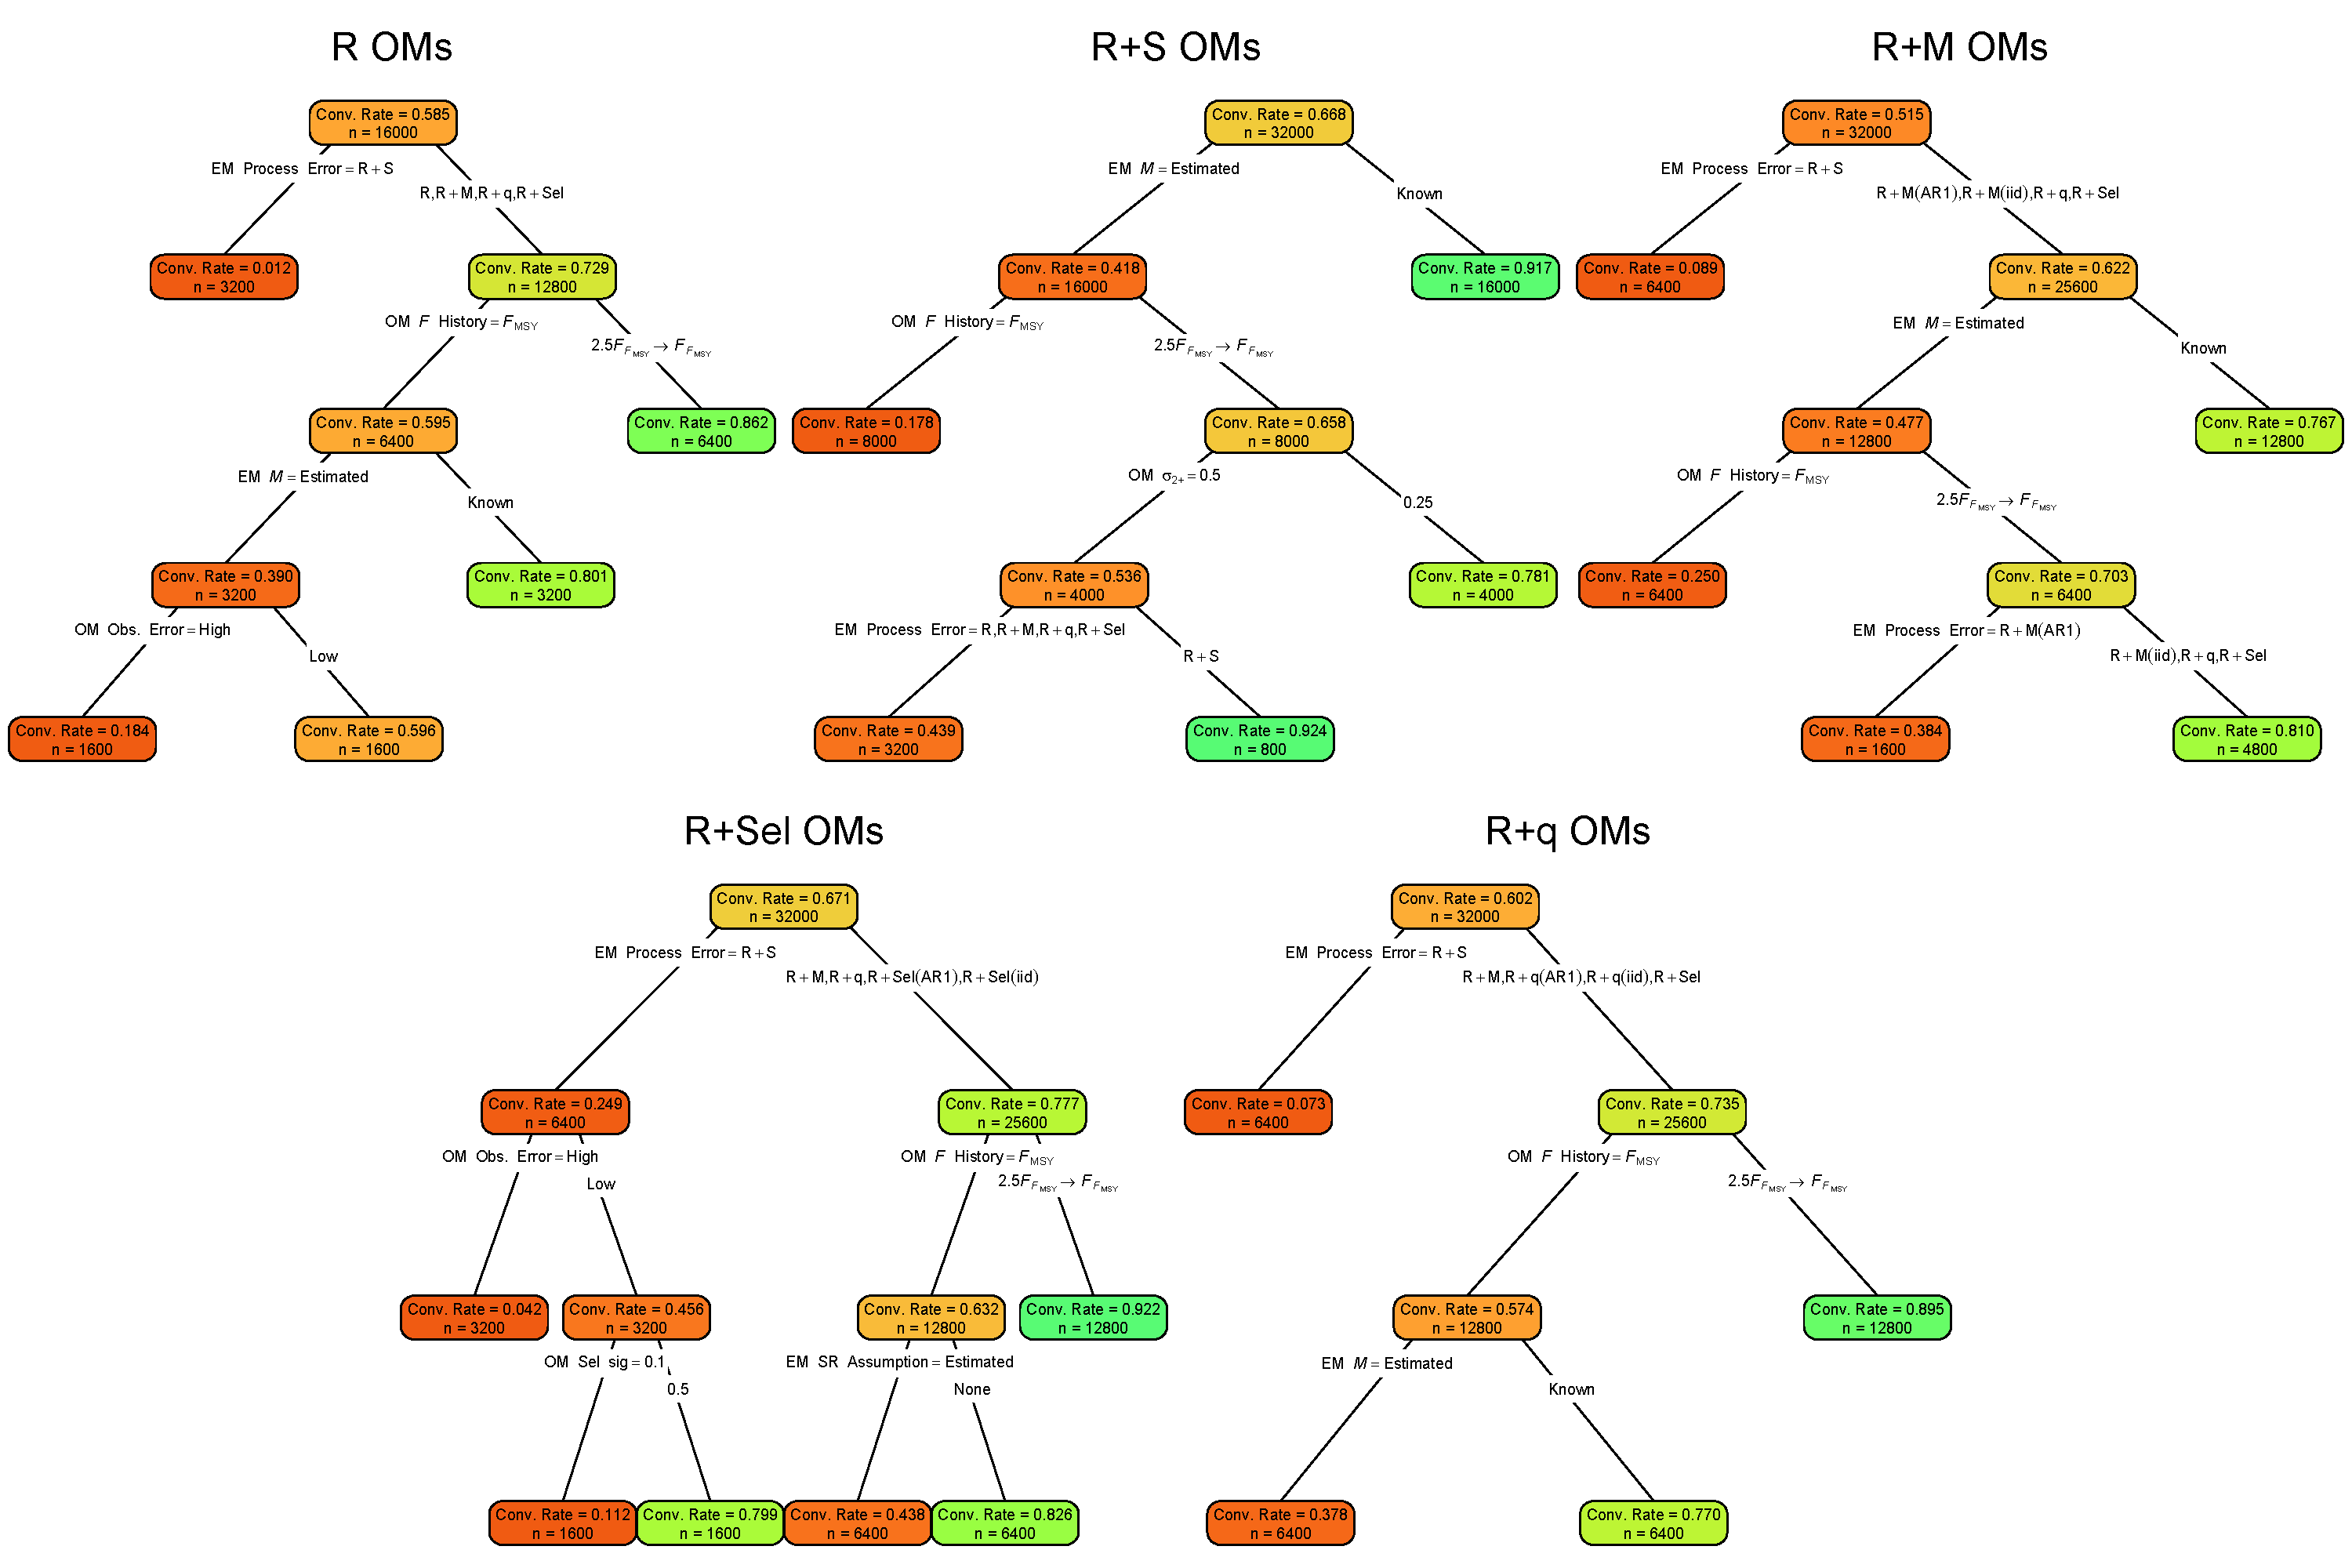
\includegraphics[width = 1.4\textwidth]{convergence_gradient_classification_plots}
\end{center}
\caption{Classification trees indicating primary factors determining convergence as defined by a maximum absolute gradient < $10^{-6}$ for R, R+S, R+M, R+Sel and R+q OMs. Nodes denote percent convergence (top) and number of fits (bottom)  for the corresponding subset. Branch labels indicate the levels of OM and EM factors distinguishing each subset and left branch labels are positioned higher and note the factor. Lower or higher convergence rates are indicated by more red or green polygons, respectively.}\label{conv_gradient_class}
\end{figure}
\end{landscape}

\begin{landscape}
\begin{figure}
\begin{center}
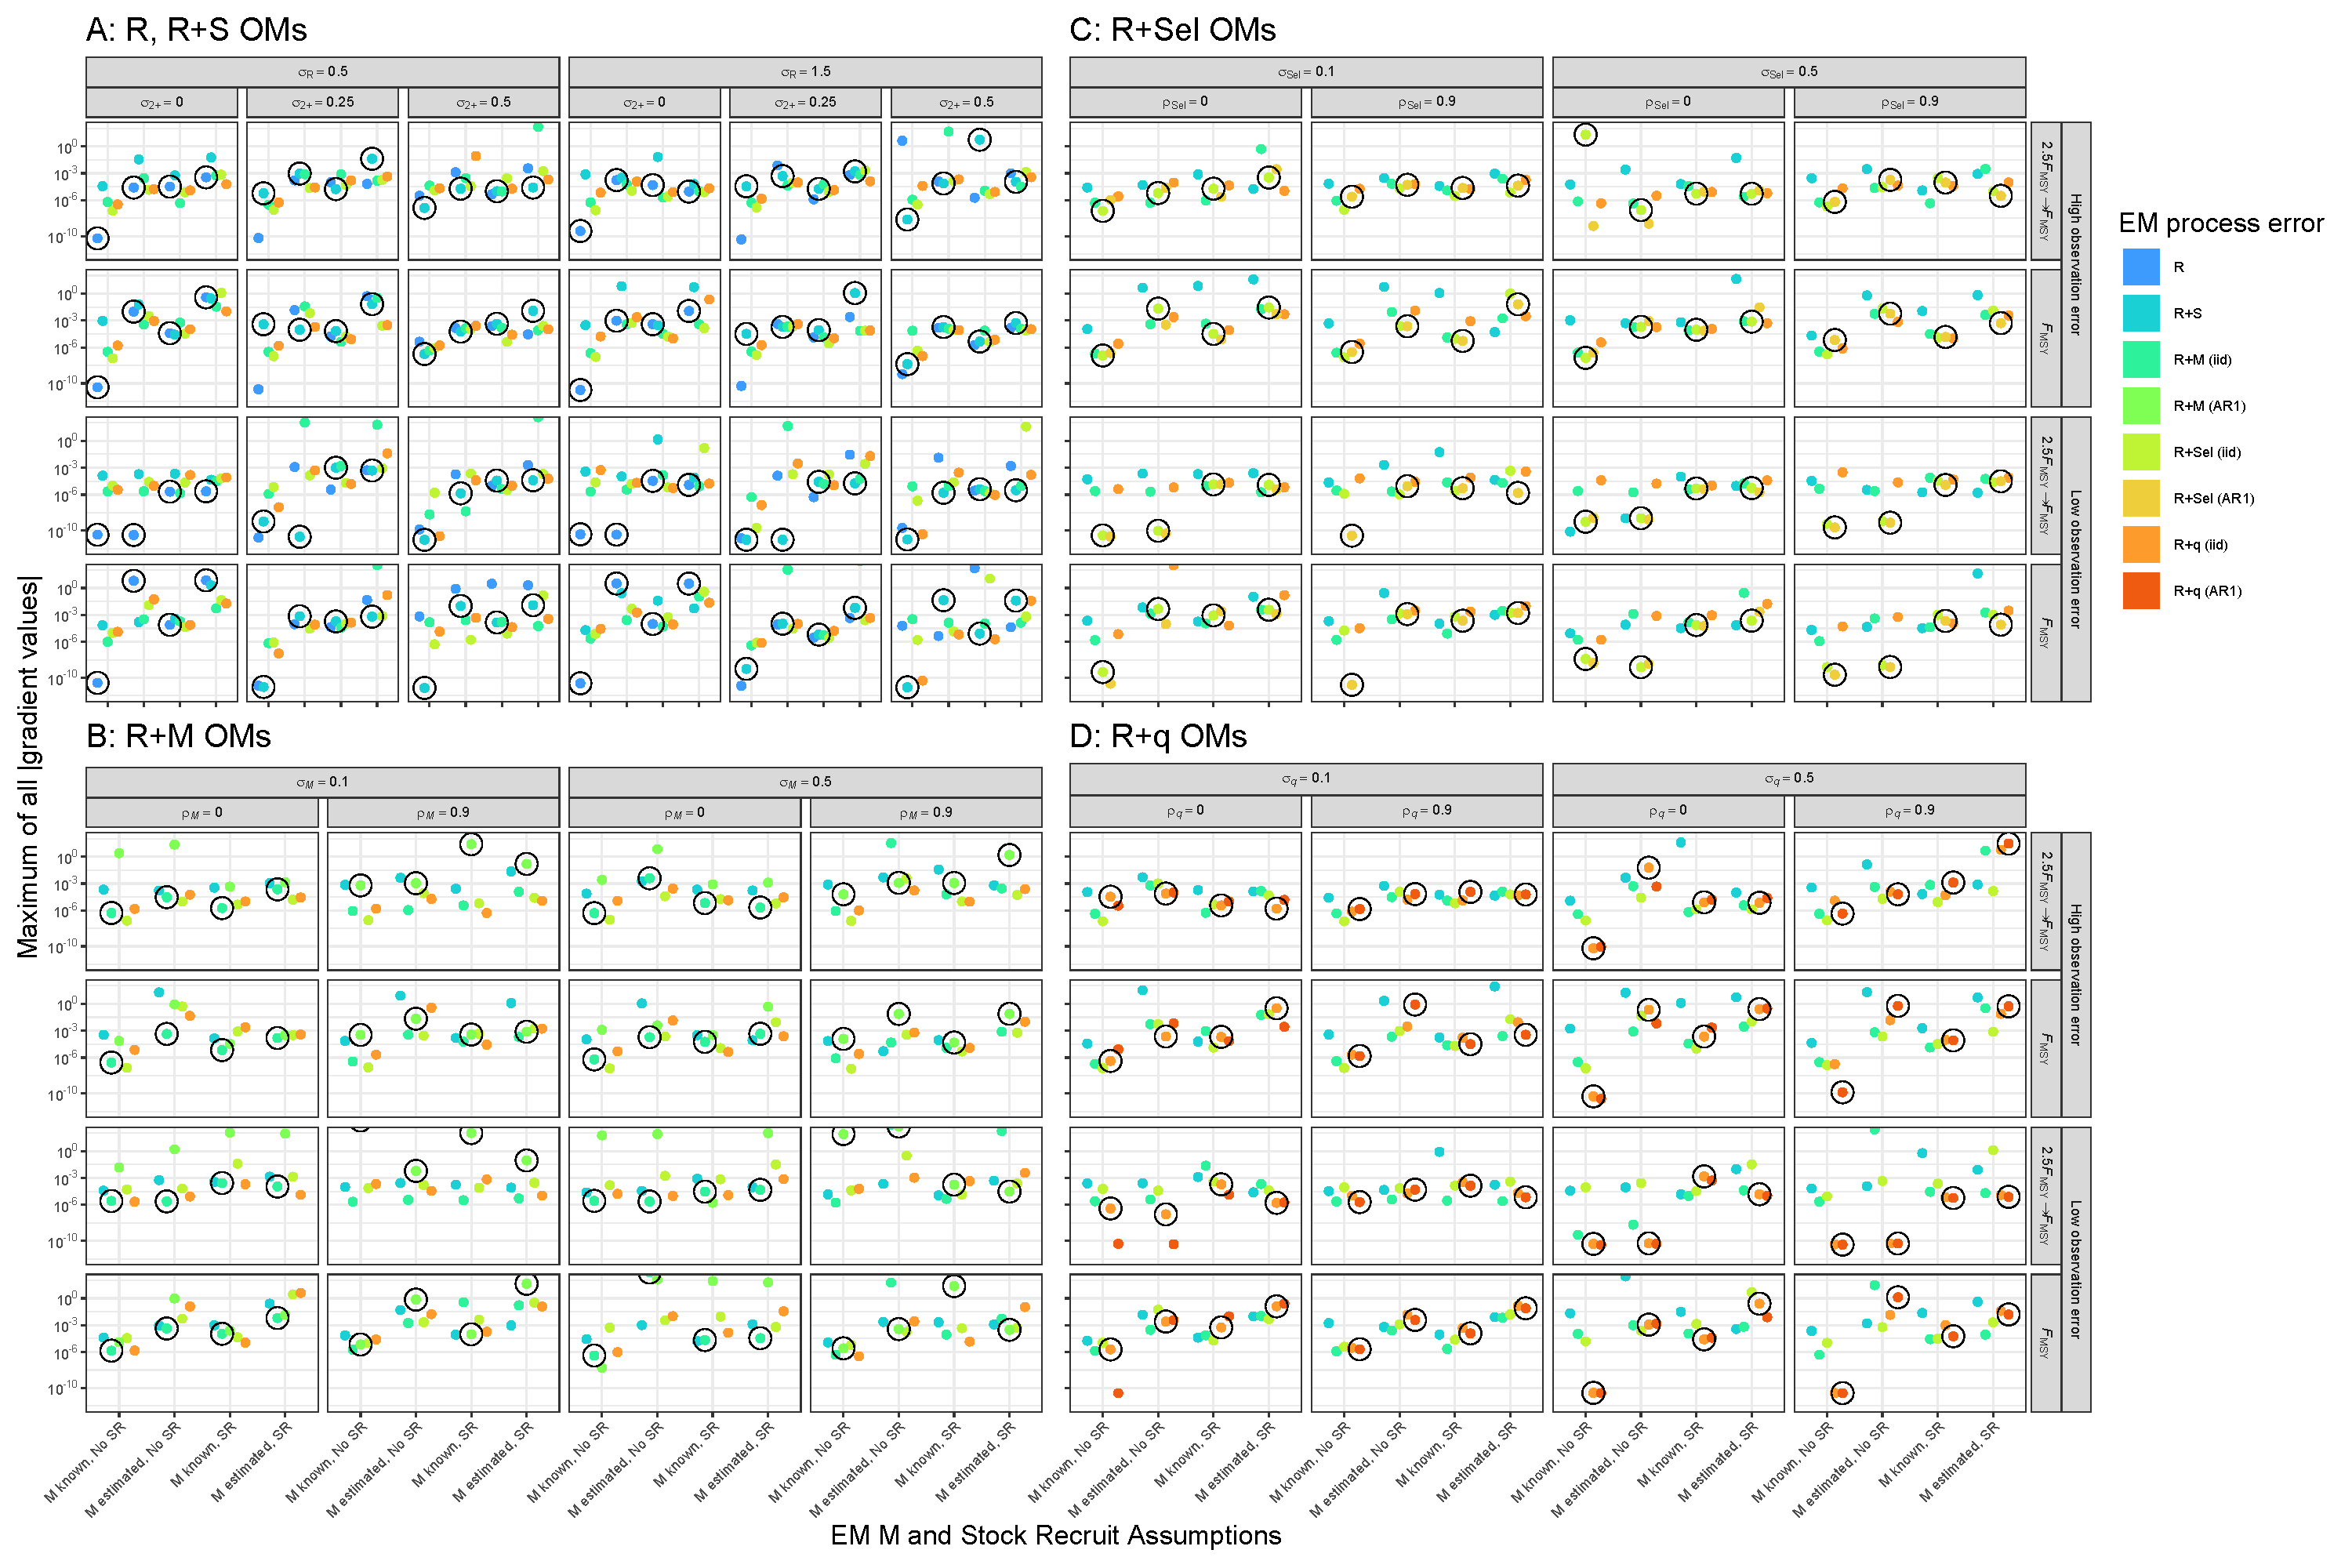
\includegraphics[width = 1.4\textwidth]{hess_grad_convergence_plots}
\end{center}
\caption{The maximum of the absolute values of all gradient values for all fits that provided Hessian-based standard errors across all simuated data sets of a given OM configuration (A: R and R+S, B: R+M, C: R+Sel, or D: R+q).  Results are conditional on EM fits with alternative process error assumptions (colored points and lines), median natural mortality rate(estimated or known) and recruitment assumptions (Beverton-Holt SRR or not). Circled values indicate results where the EM process error structure matches that of the OM and vertical lines represent 95\% confidence intervals.}\label{hess_grad}
\end{figure}
\end{landscape}

\begin{landscape}
\begin{figure}
\begin{center}
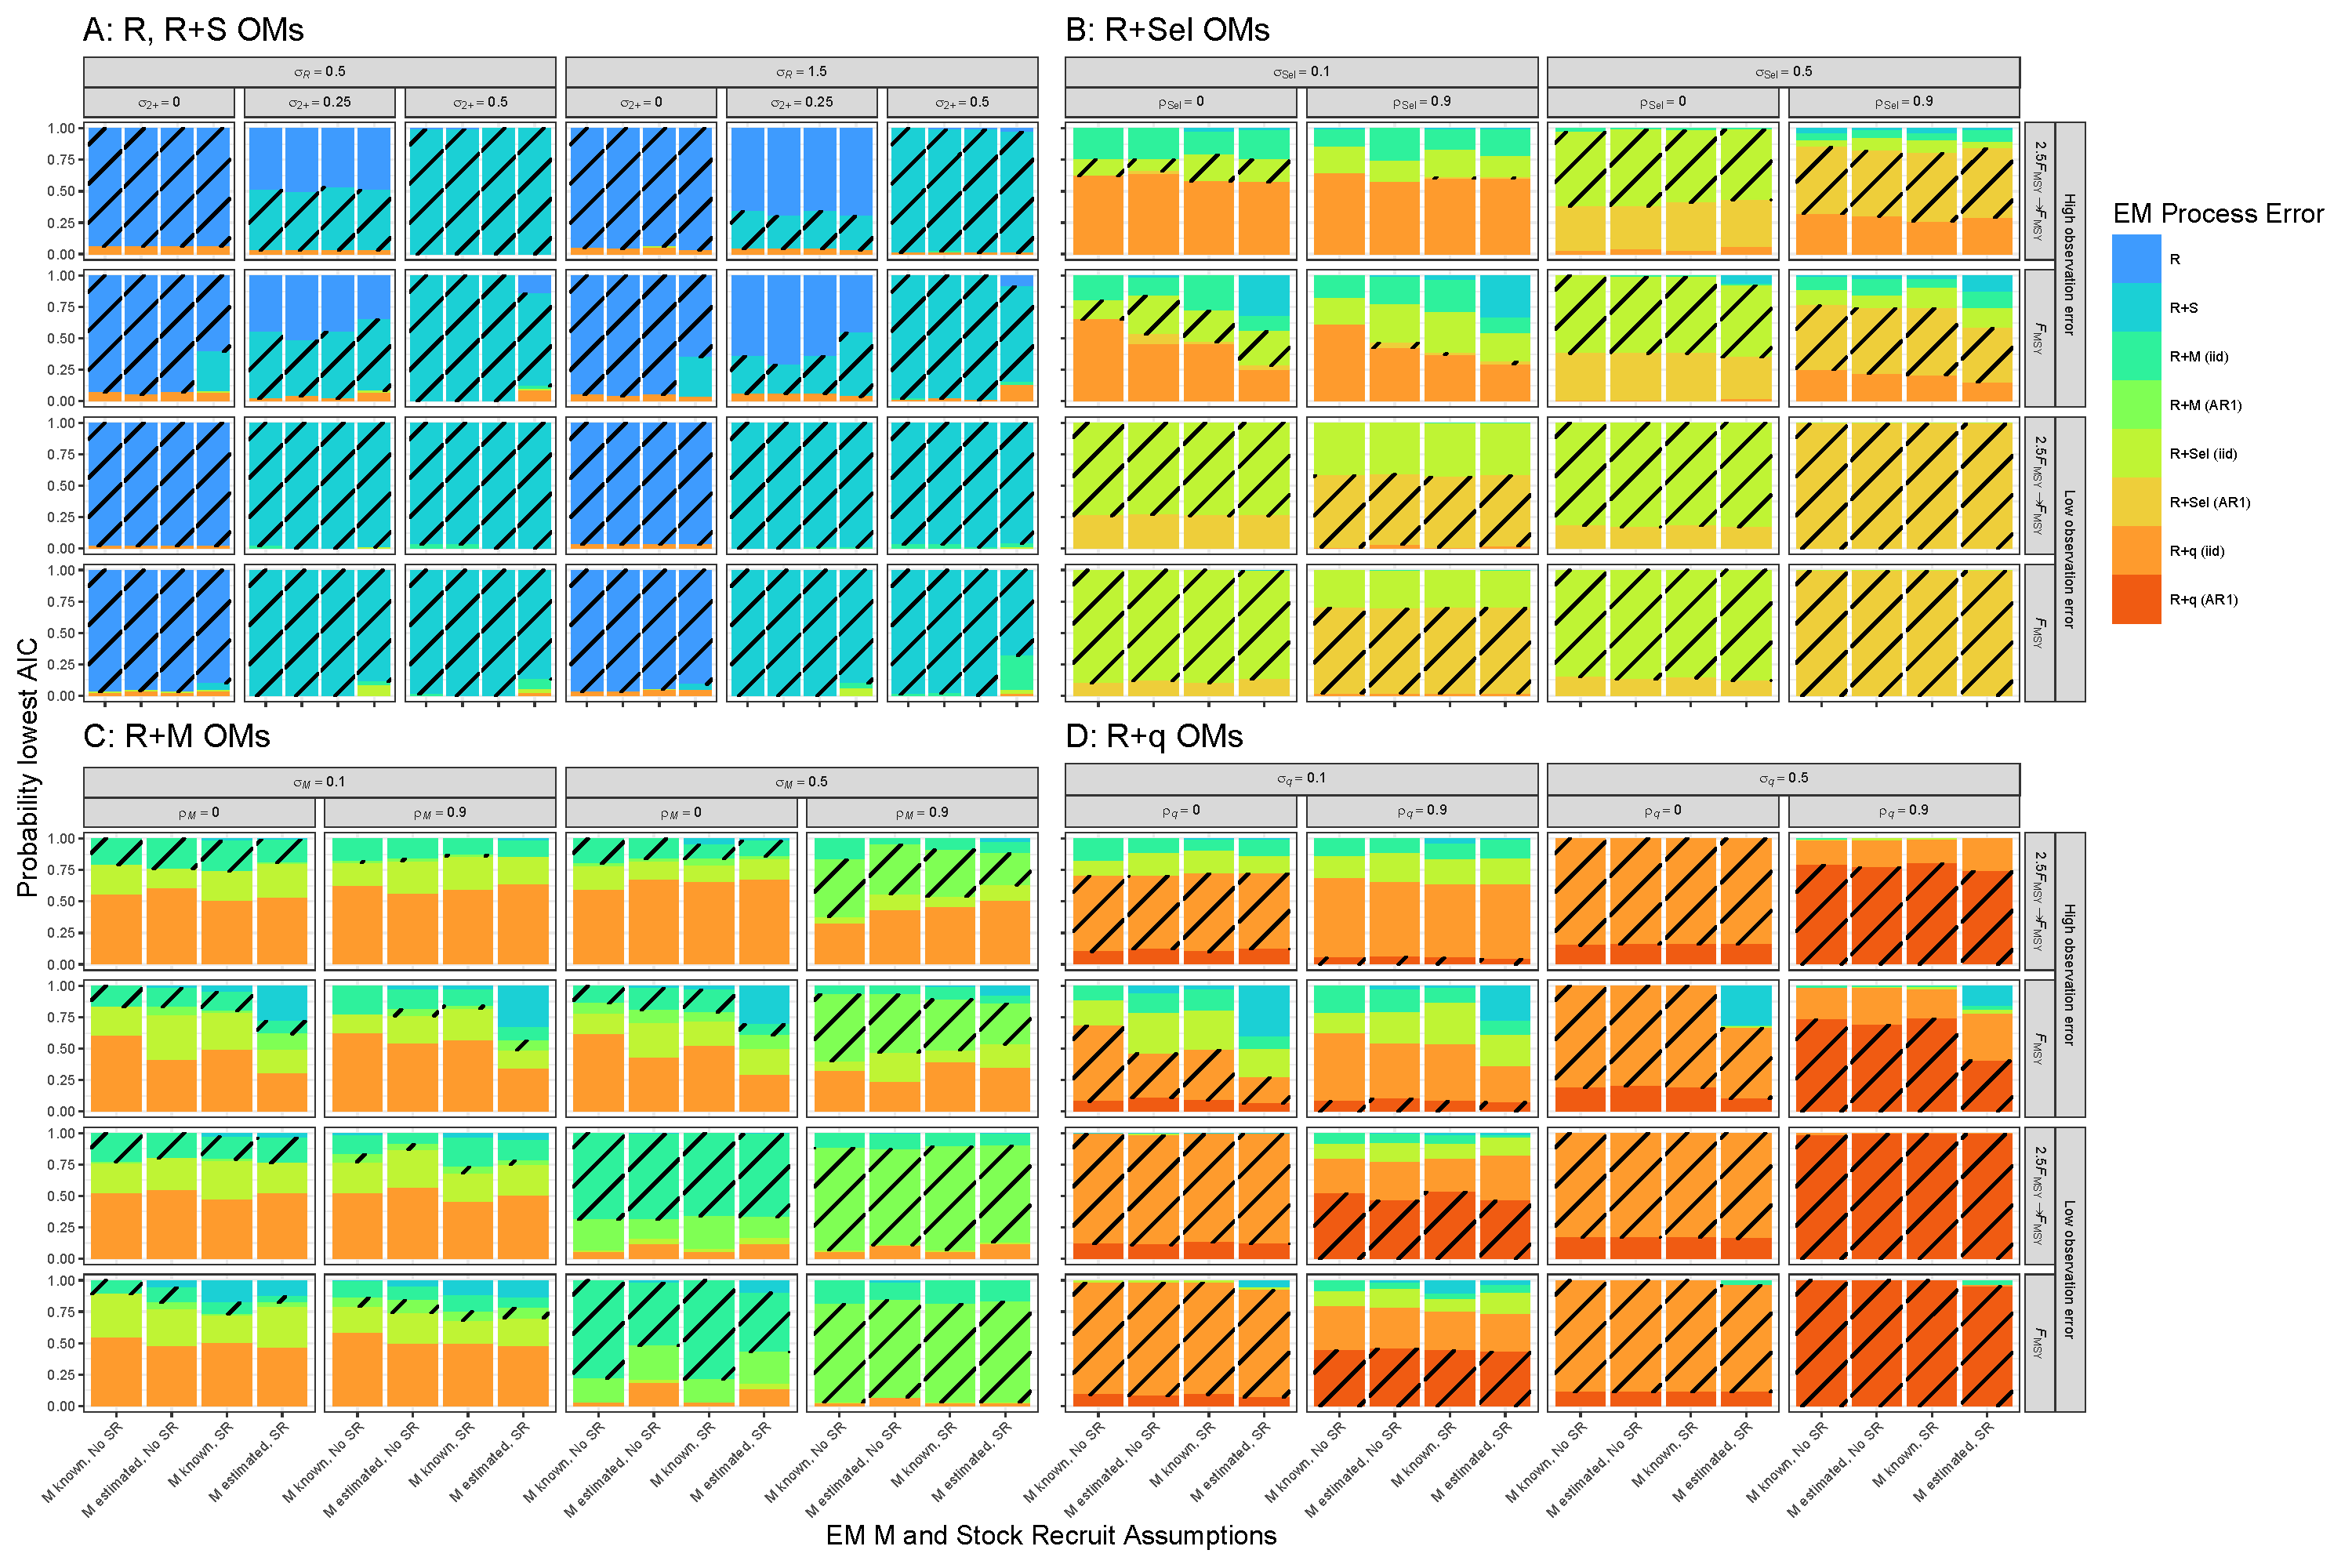
\includegraphics[width = 1.4\textwidth]{pe_aic_plots}
\end{center}
\caption{Estimated probability of lowest AIC for EMs assuming alternative process error assumptions (colored bars) conditional on alternative assumptions for median natural mortality rate (estimated or known) and Beverton-Holt SRR (estimated or not; along x-axis) when fitted to OMs that have R and R+S (A), R+Sel (B), R+M (C), or R+q (D) process error sources. Striped bars indicate results where the EM process error structure matches that of the OM.}\label{pe_aic}
\end{figure}
\end{landscape}

\begin{landscape}
\begin{figure}
\begin{center}
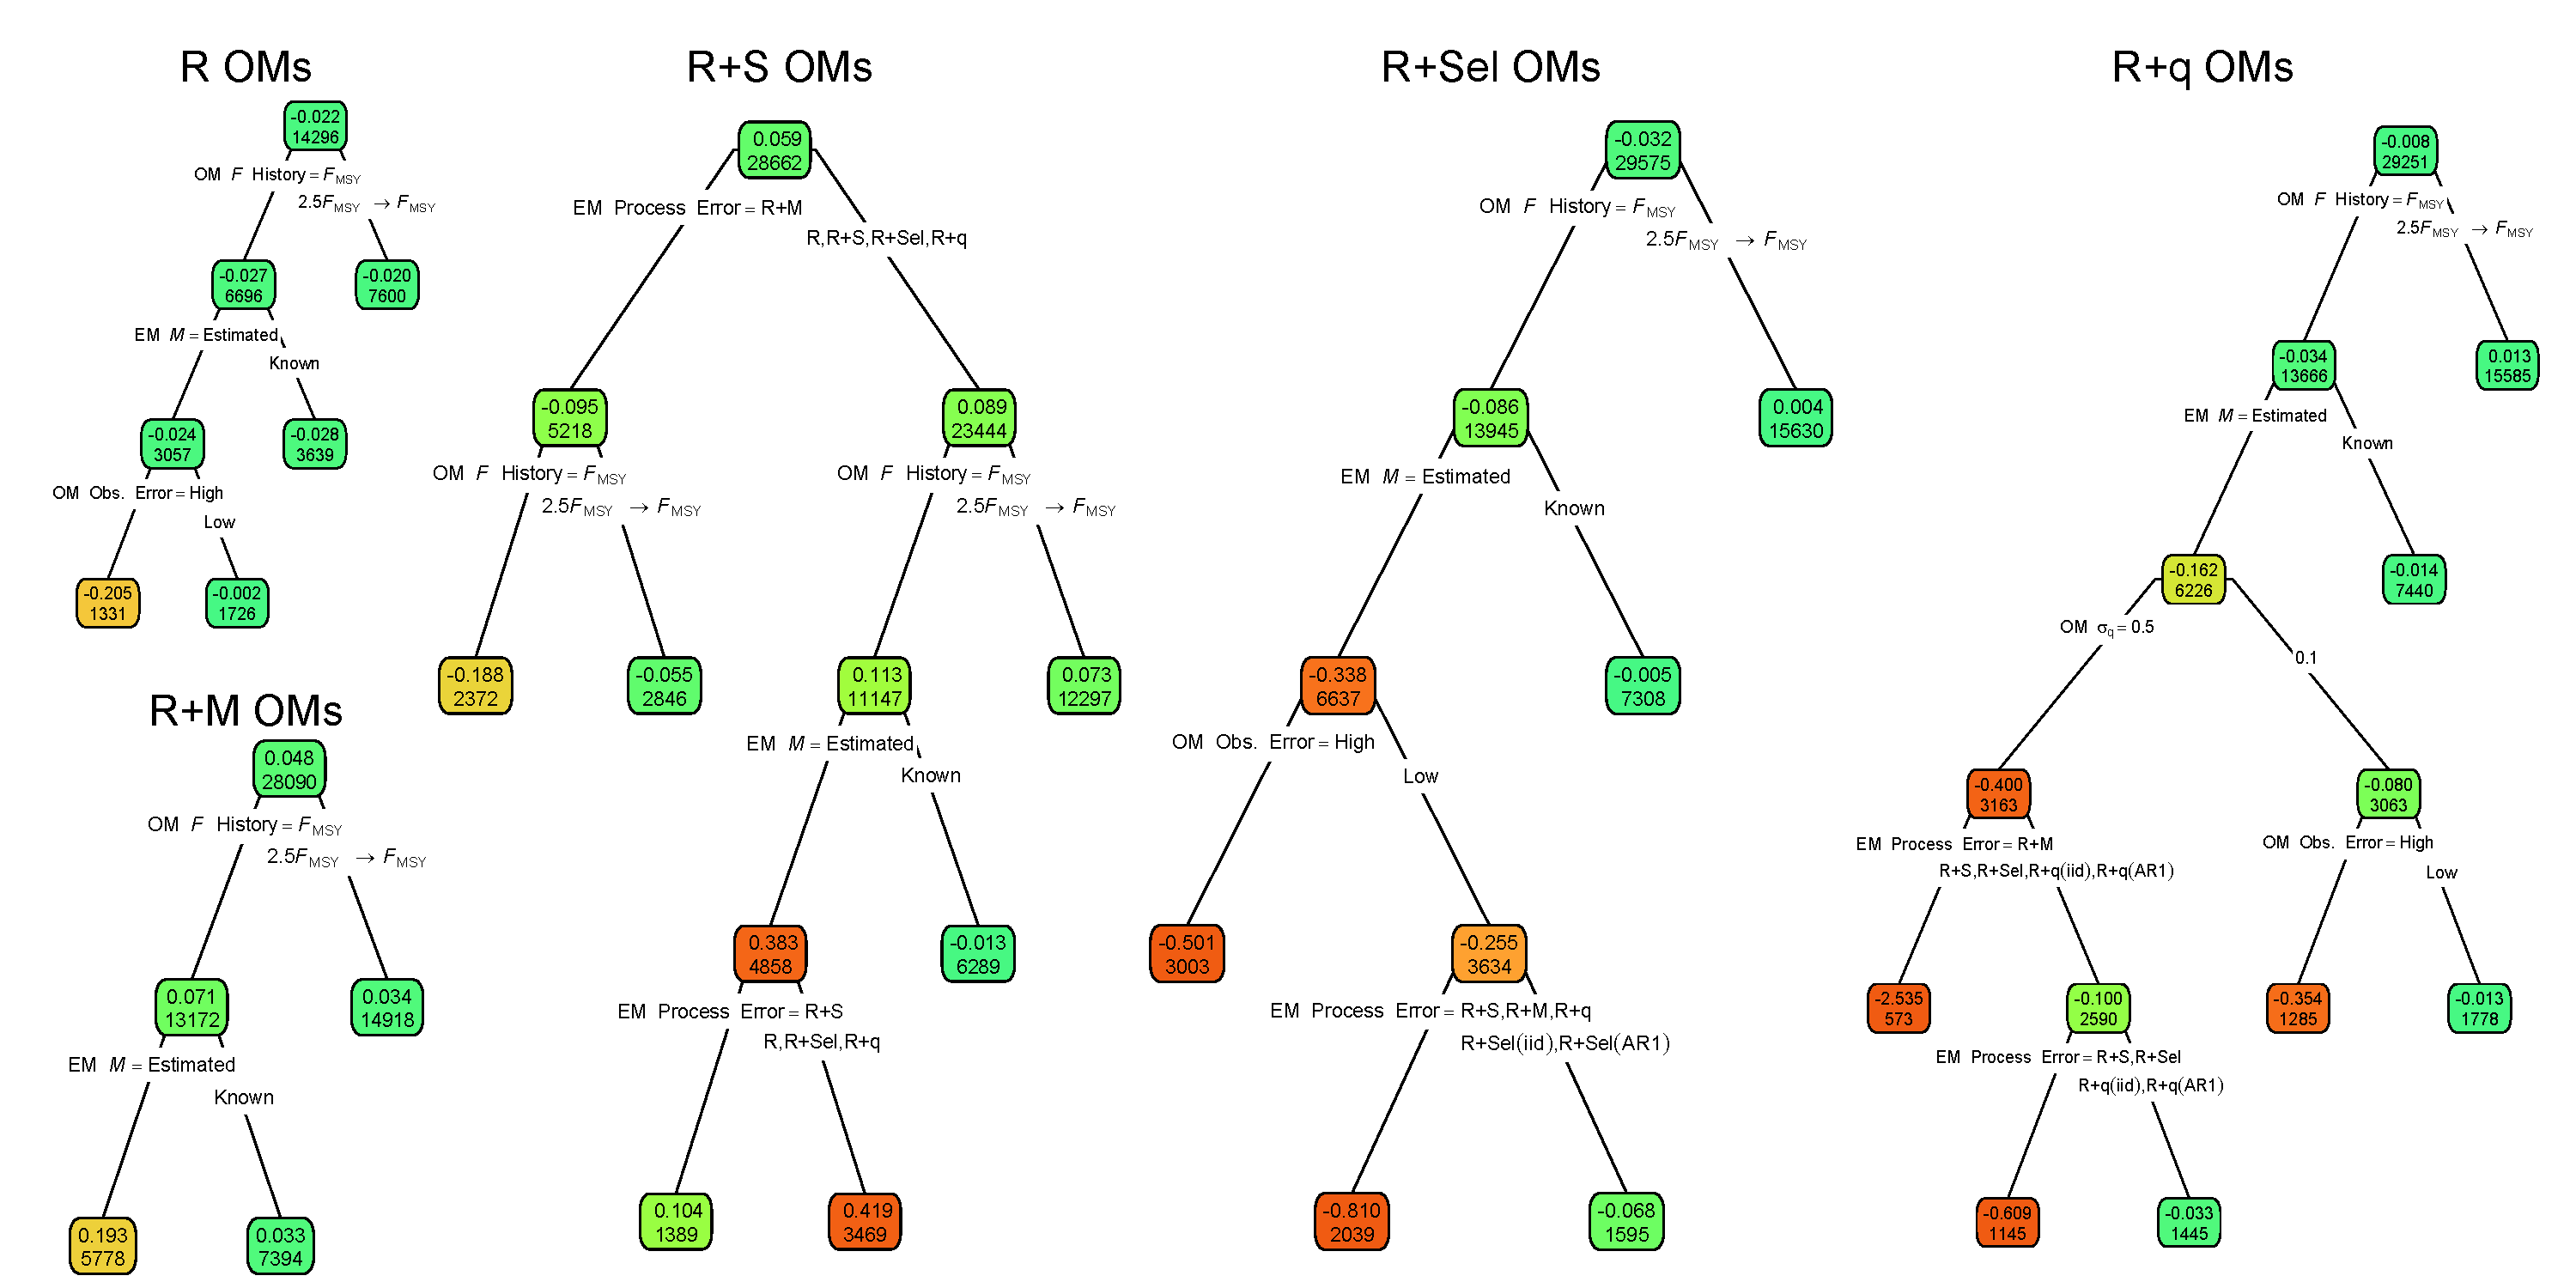
\includegraphics[width = 1.4\textwidth]{F_bias_regtree_plots}
\end{center}
\caption{Regression trees indicating primary factors determining reductions in sums of squares of errors in estimation measured by Eq. 3 for terminal year fully-selected fishing mortality for R+S, R+M, R+Sel and R+q OMs. Each node shows the median error (top) and number of observations (bottom) for the corresponding subset. Branch labels indicate the levels of OM and EM factors distinguishing each subset and left branch labels are positioned higher and note the factor. Median errors closer to or further from zero are indicated by more green or red polygons, respectively.}\label{F_bias_regtree}
\end{figure}
\end{landscape}

\begin{landscape}
\begin{figure}
\begin{center}
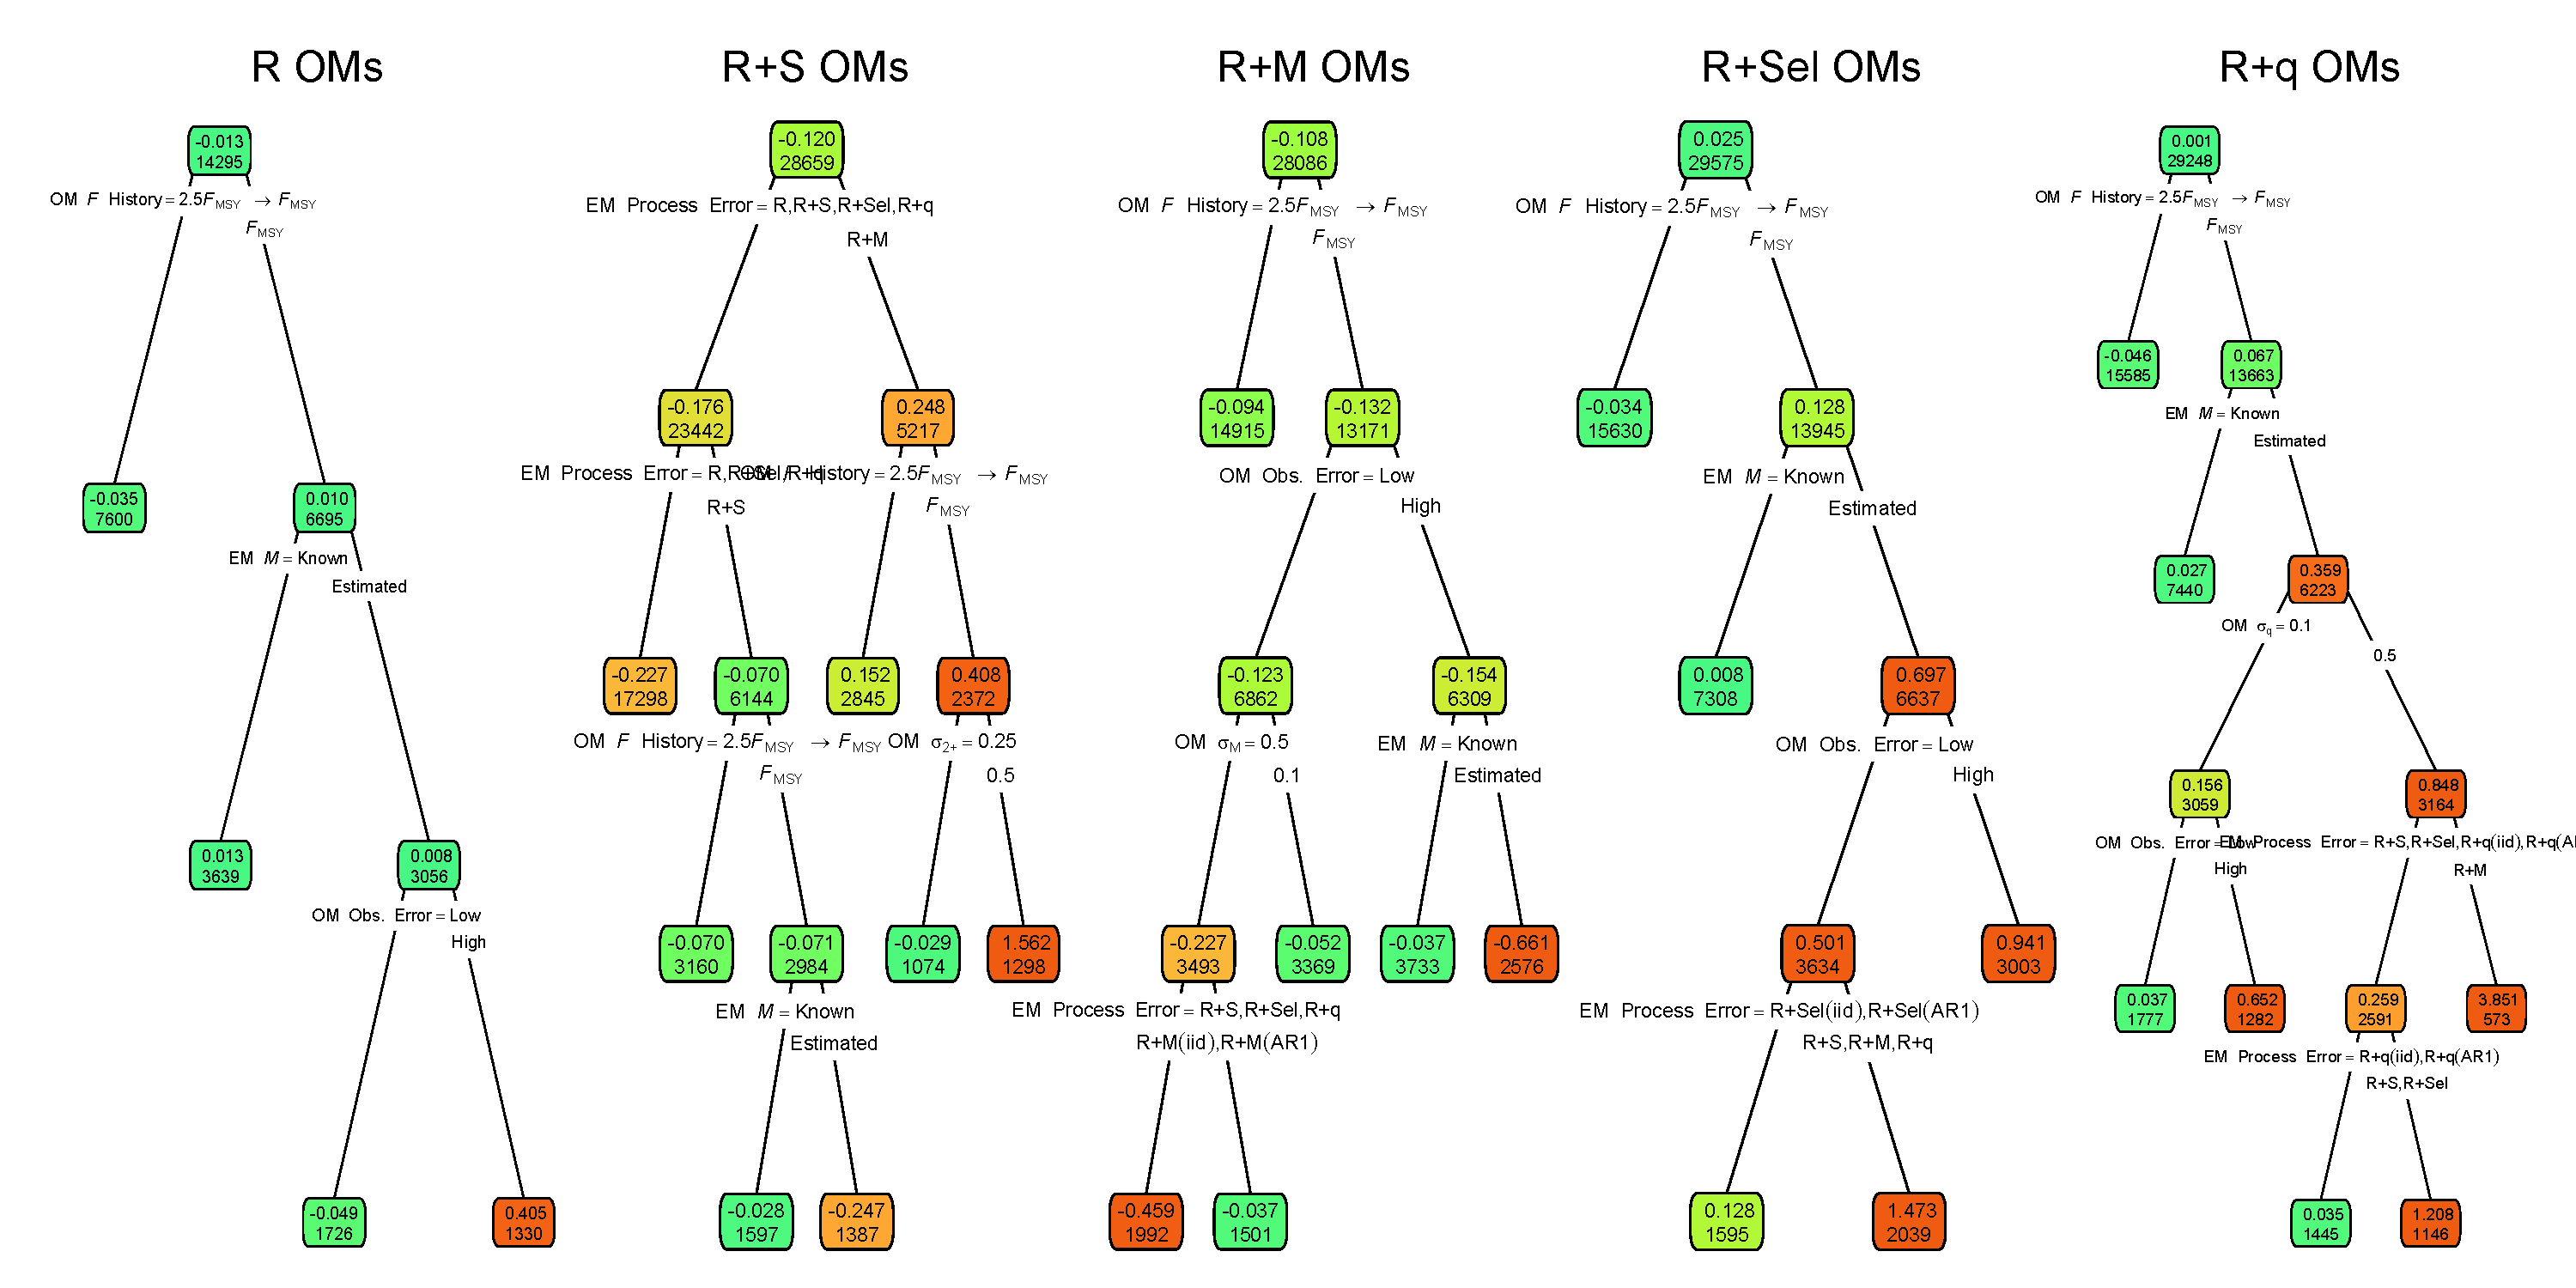
\includegraphics[width = 1.4\textwidth]{R_bias_regtree_plots}
\end{center}
\caption{Regression trees indicating primary factors determining reductions in sums of squares of errors in estimation measured by Eq. 3 for terminal year recruitment for R+S, R+M, R+Sel and R+q OMs. Each node shows the median error (top) and number of observations (bottom) for the corresponding subset. Branch labels indicate the levels of OM and EM factors distinguishing each subset and left branch labels are positioned higher and note the factor. Median errors closer to or further from zero are indicated by more green or red polygons, respectively.}\label{R_bias_regtree}
\end{figure}
\end{landscape}

\begin{landscape}
\begin{figure}
\begin{center}
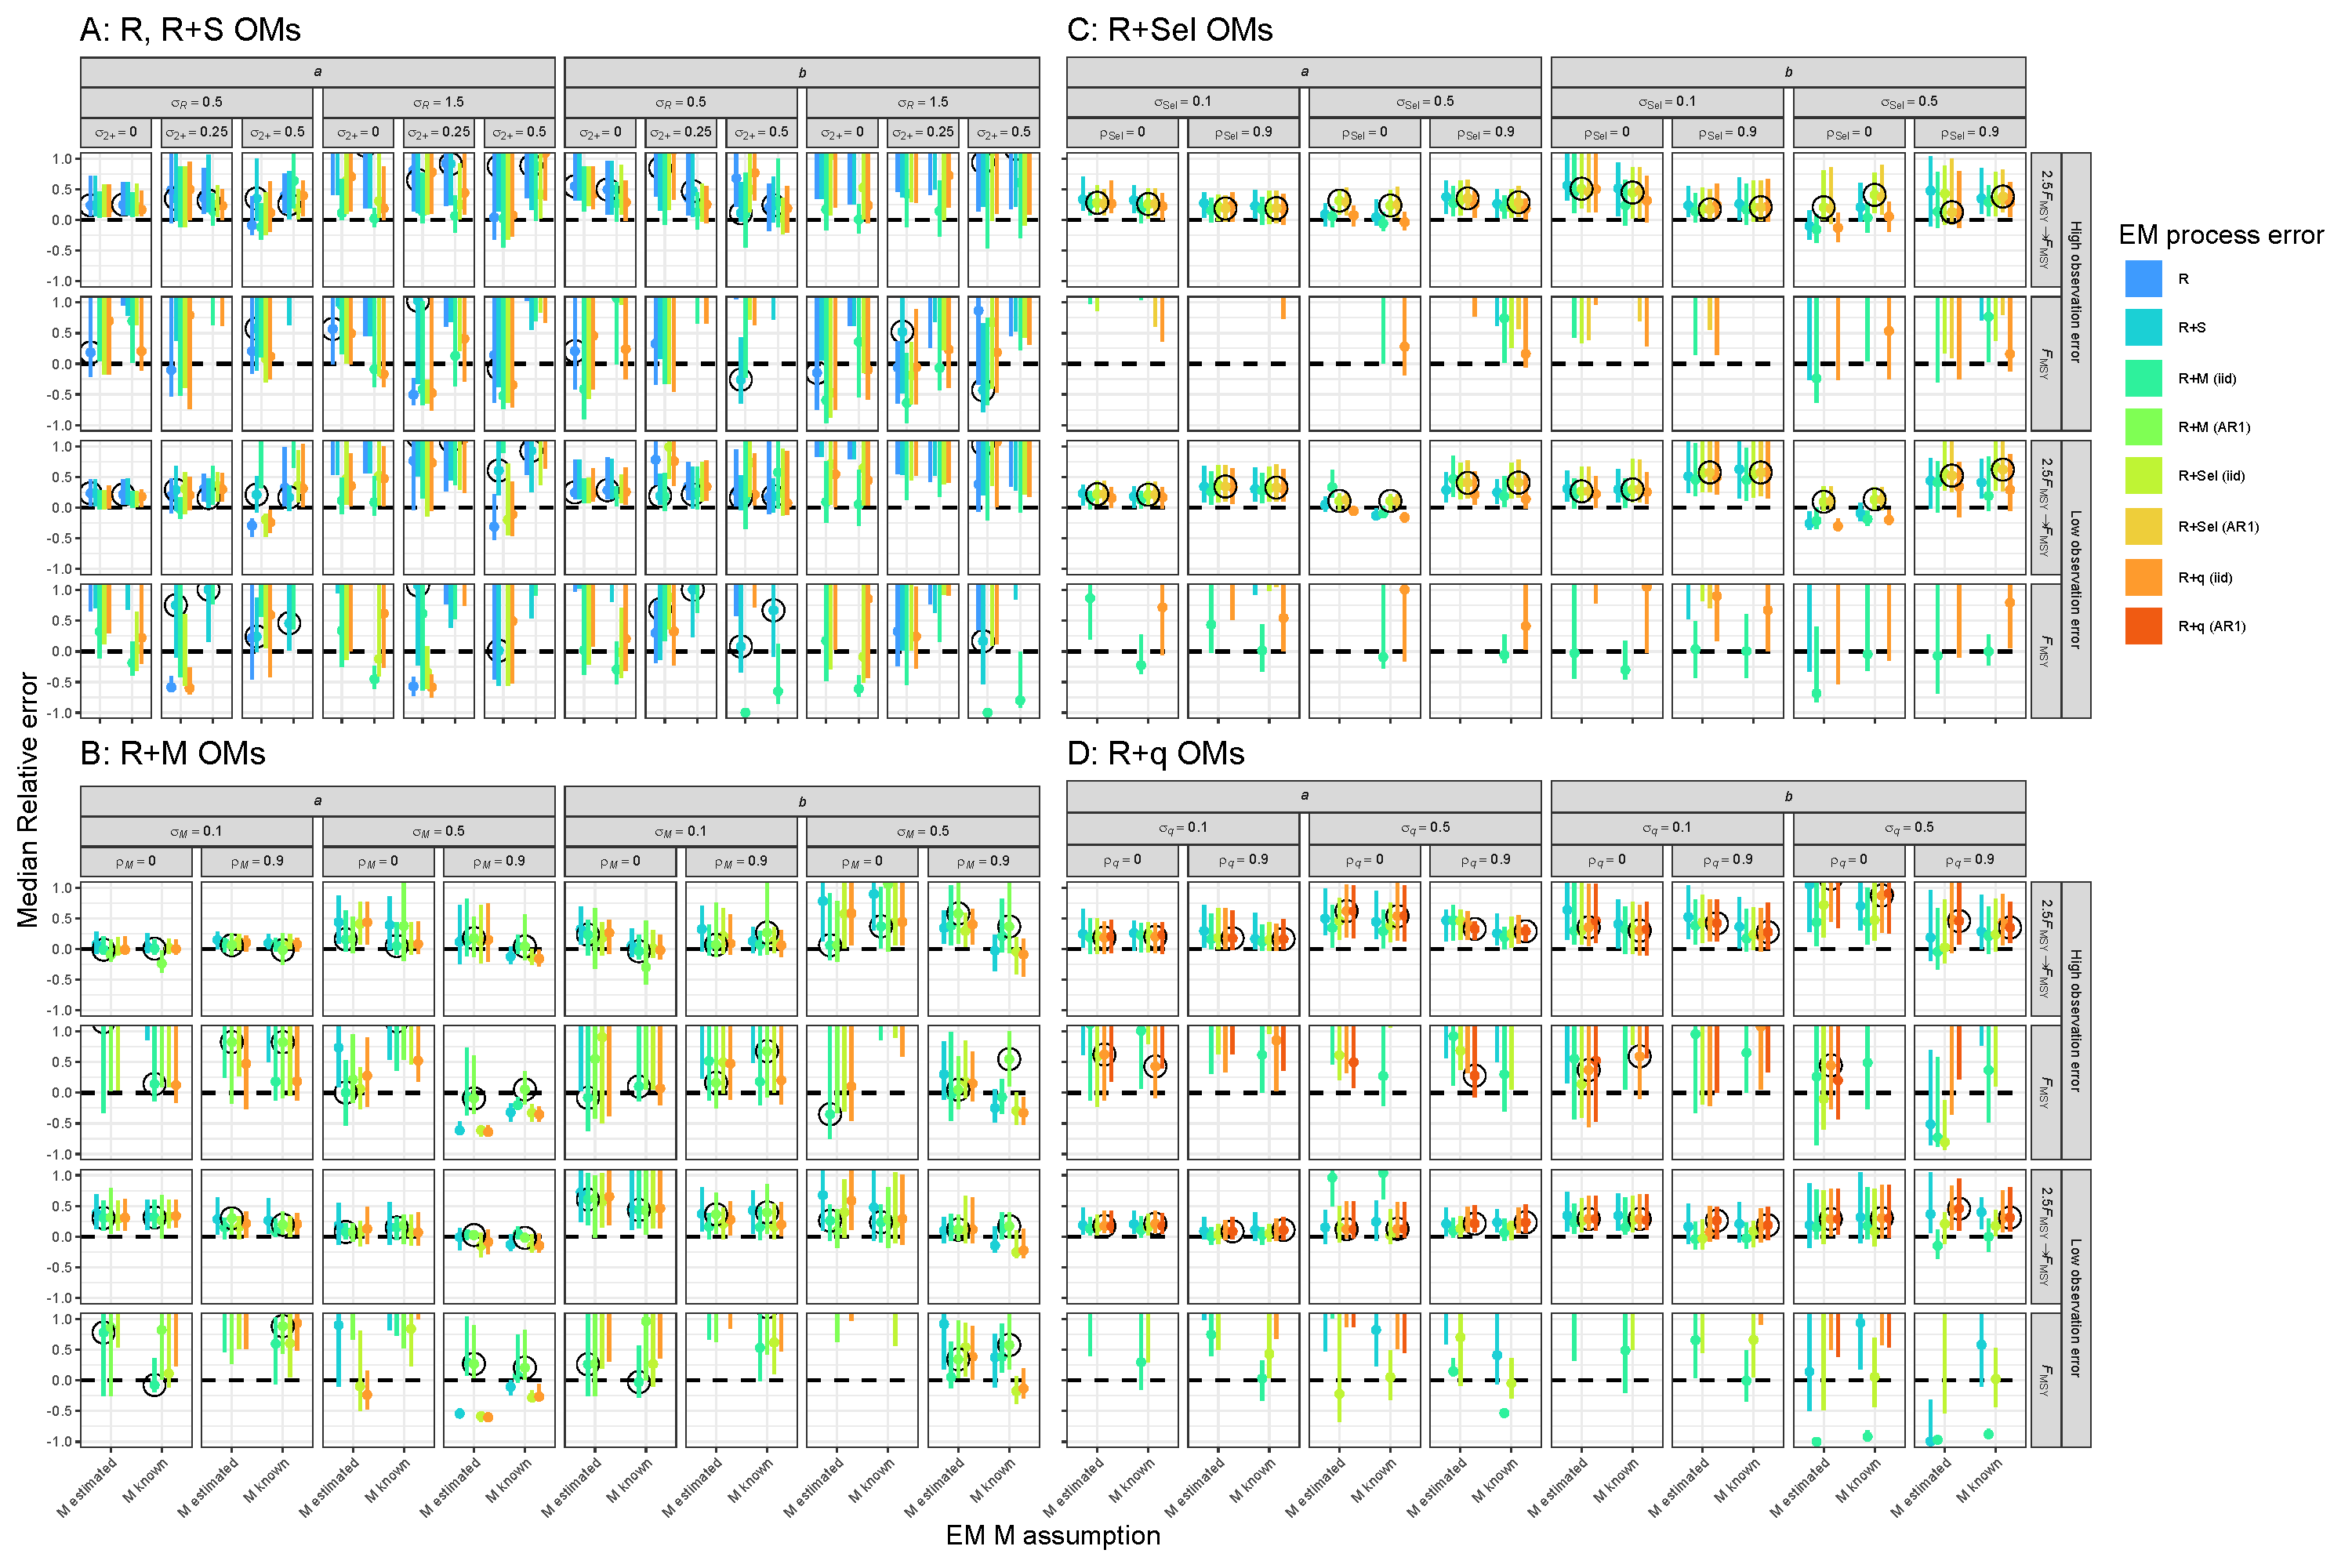
\includegraphics[width = 1.4\textwidth]{sr_bias_plots}
\end{center}
\caption{Median relative error of Beverton-Holt SRR parameters ($a = \alpha$ and $b = \beta$) for EMs fitted to data sets simulated with alternative process error structures: R and R+S (A), R+Sel (B), R+M (C), or R+q (D). Circled values indicate results where the EM process error structure matches that of the OM and vertical lines represent 95\% confidence intervals.}\label{SR_rel_error}
\end{figure}
\end{landscape}

\begin{landscape}
\begin{figure}
\begin{center}
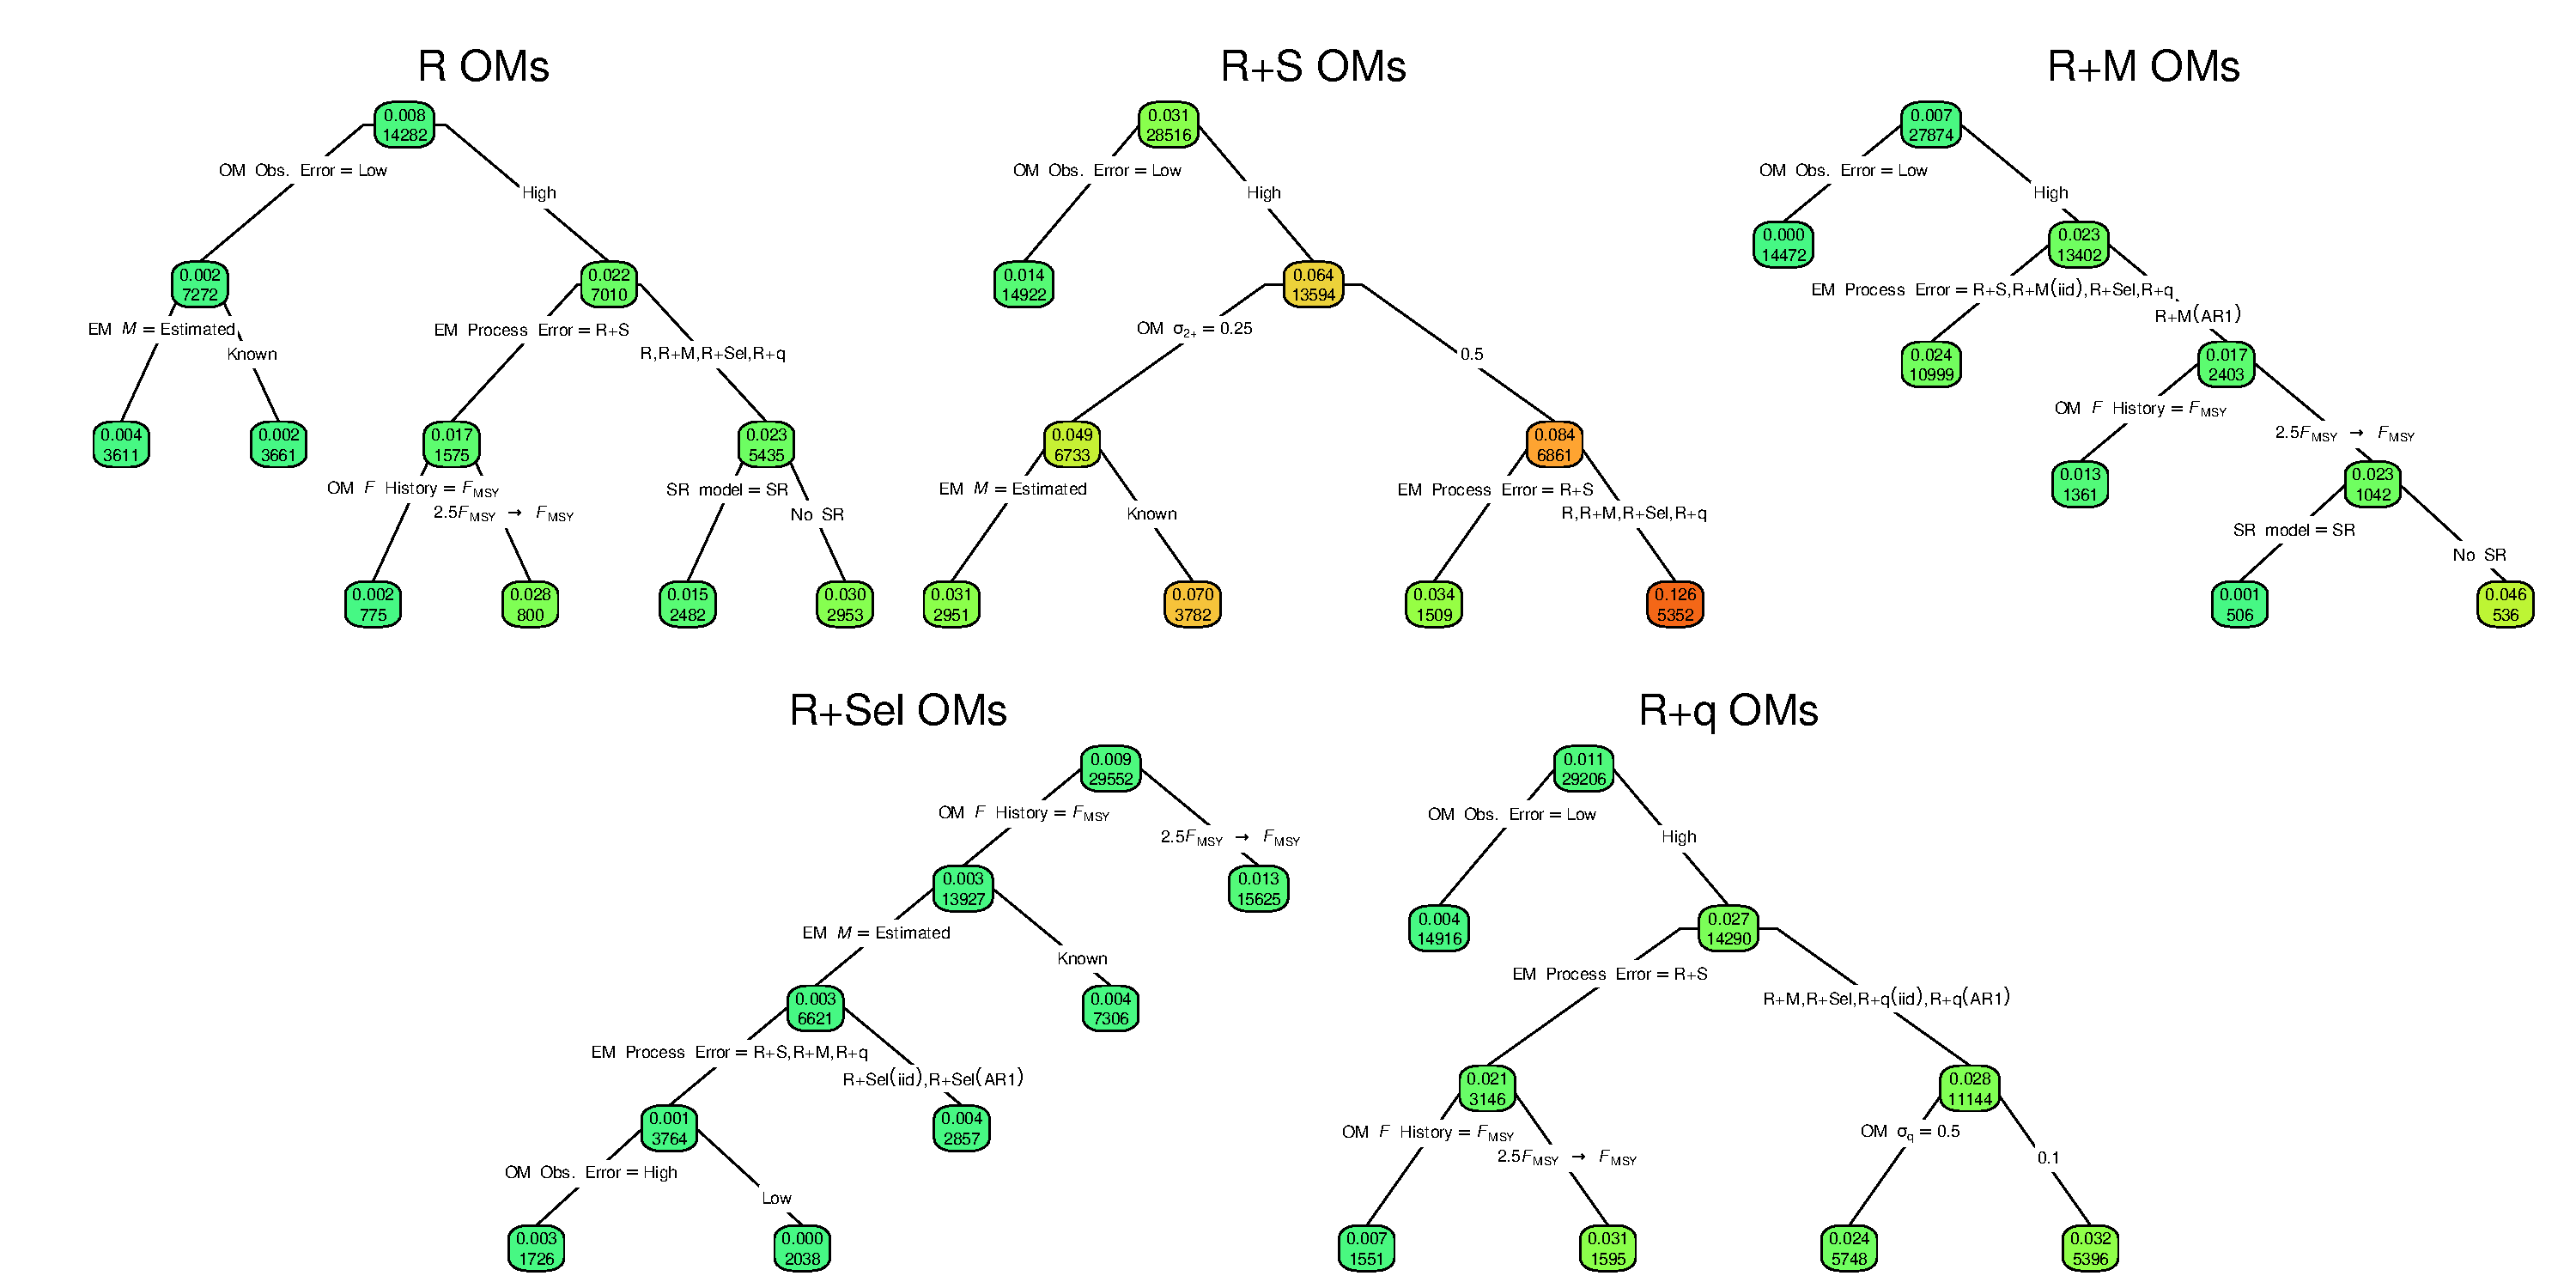
\includegraphics[width = 1.4\textwidth]{F_mohns_rho_regtree_plots}
\end{center}
\caption{Regression trees indicating primary factors determining reductions in sums of squares of errors in transformed Mohn's $\rho$ (Eq. 3) for fishing mortality averaged over all age classes for R+S, R+M, R+Sel and R+q OMs. Each node shows the median Mohn's $\rho$ (top) and number of observations (bottom) for the corresponding subset. Branch labels indicate the levels of OM and EM factors distinguishing each subset and left branch labels are positioned higher and note the factor. Median Mohn's $\rho$ closer to or further from zero are indicated by more green or red polygons, respectively.}\label{F_mohns_rho_regtree}
\end{figure}
\end{landscape}

\begin{landscape}
\begin{figure}
\begin{center}
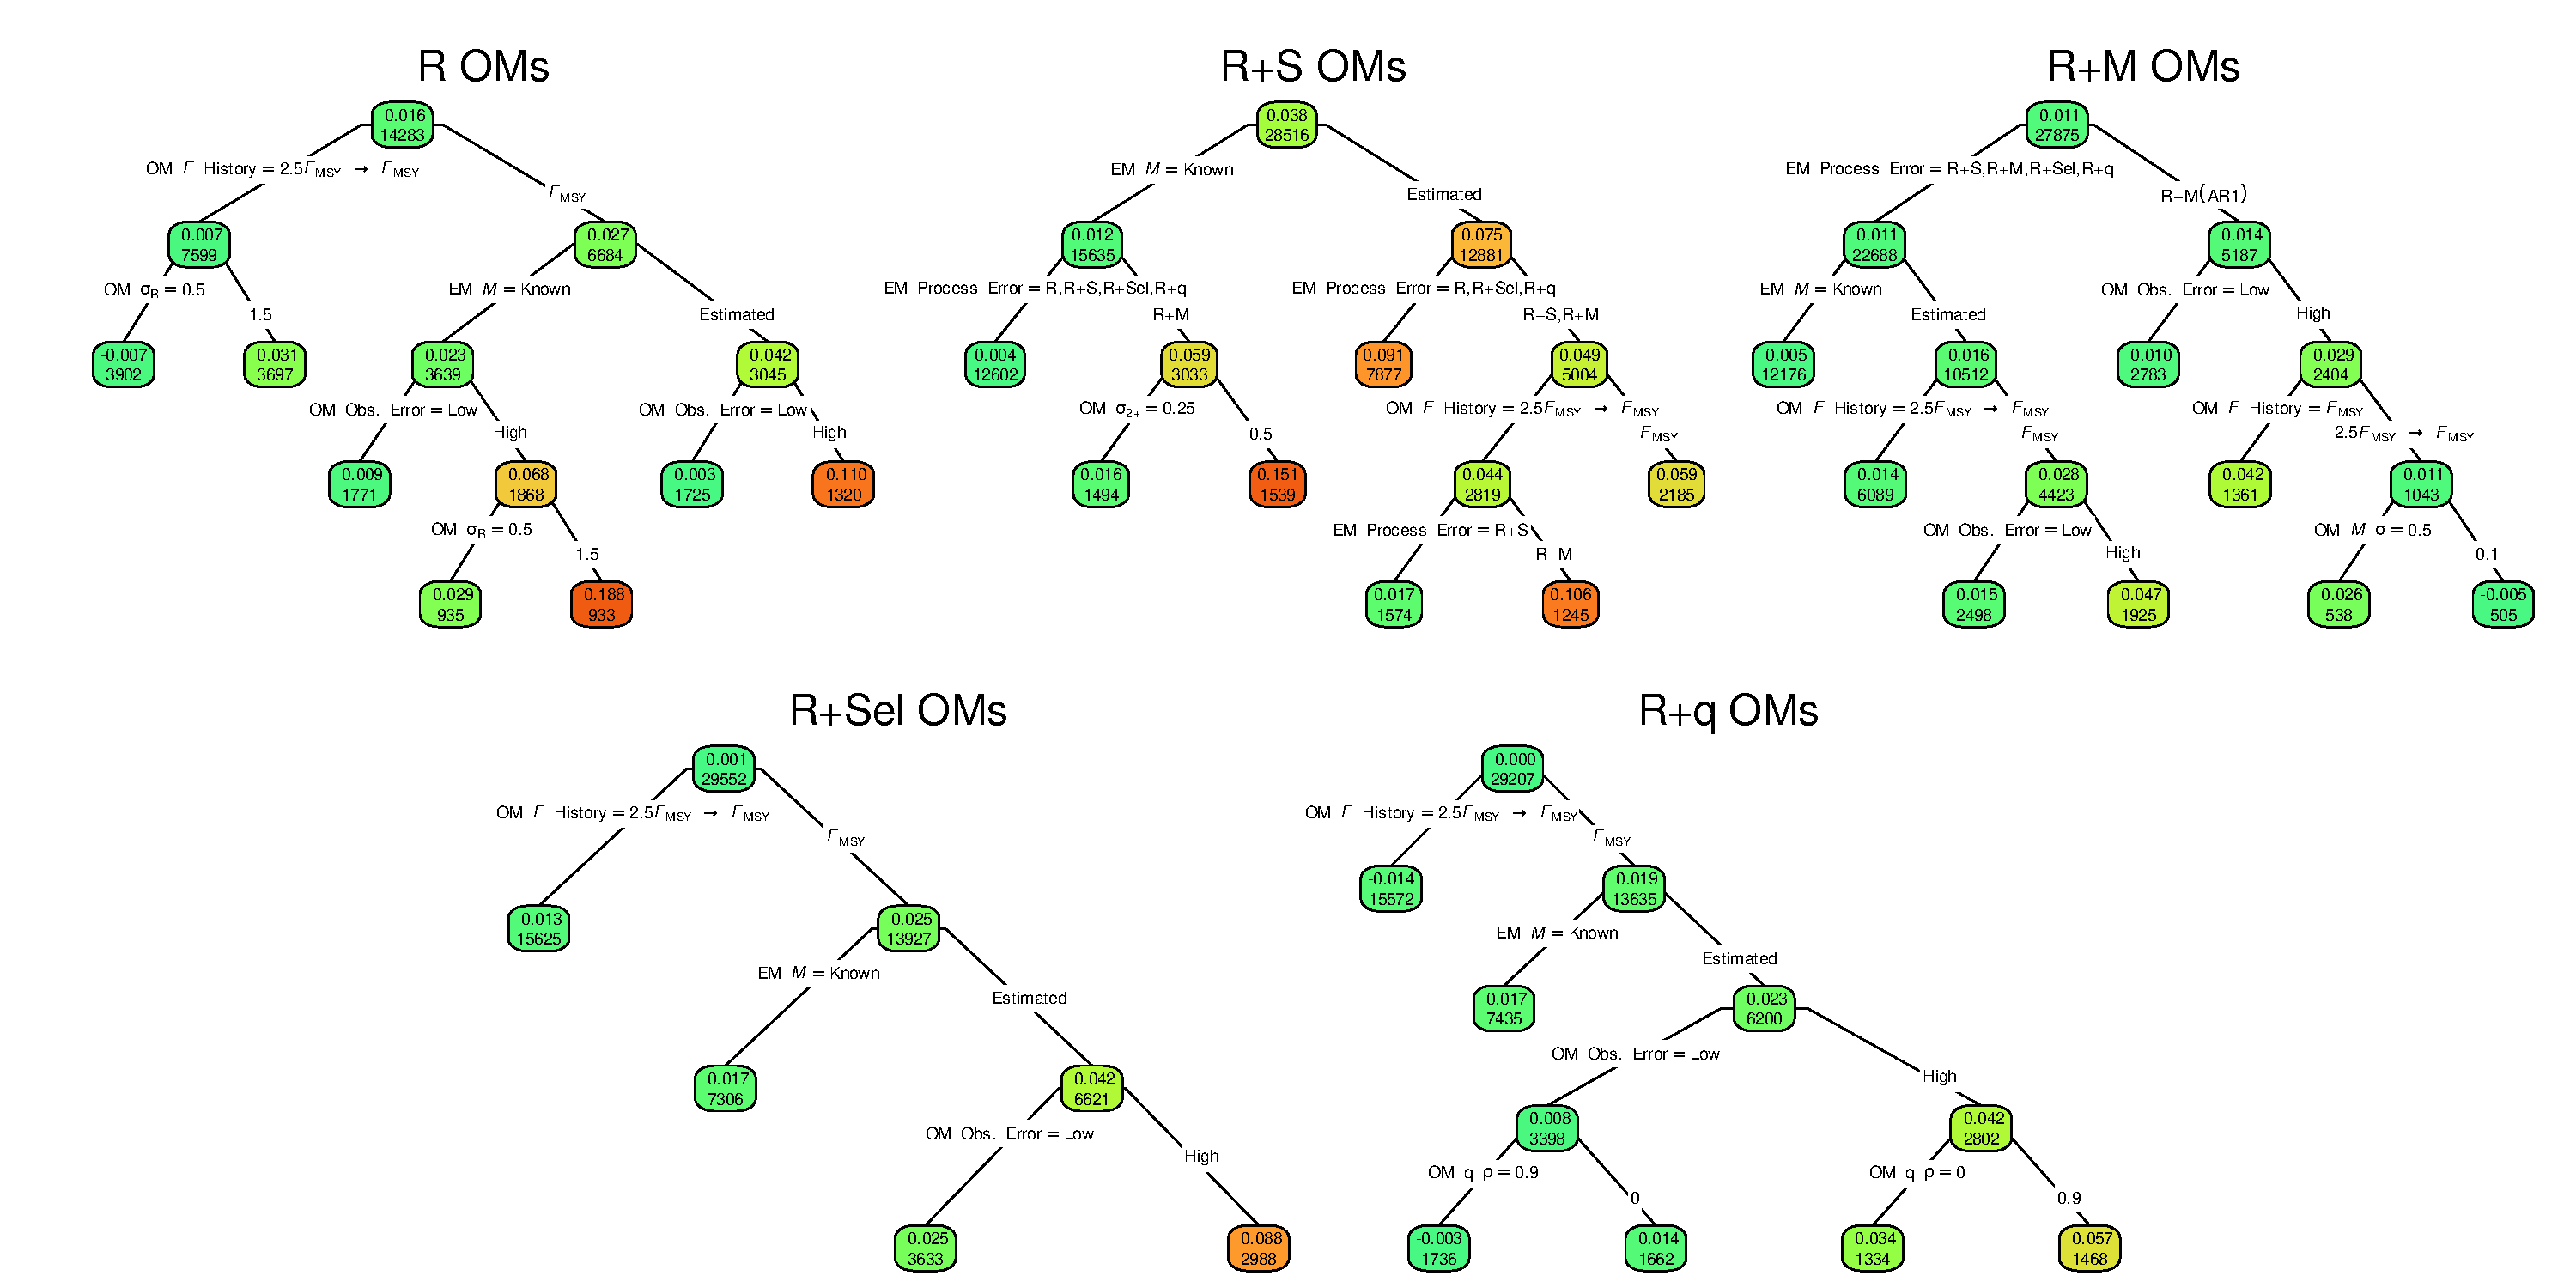
\includegraphics[width = 1.4\textwidth]{R_mohns_rho_regtree_plots}
\end{center}
\caption{Regression trees indicating primary factors determining reductions in sums of squares of errors in transformed Mohn's $\rho$ (Eq. 3) for recruitment for R+S, R+M, R+Sel and R+q OMs. Each node shows the median Mohn's $\rho$ (top) and number of observations (bottom) for the corresponding subset. Branch labels indicate the levels of OM and EM factors distinguishing each subset and left branch labels are positioned higher and note the factor. Median Mohn's $\rho$ closer to or further from zero are indicated by more green or red polygons, respectively.}\label{R_mohns_rho_regtree}
\end{figure}
\end{landscape}

\section*{Referenced Tables}\label{referenced-tables}
\addcontentsline{toc}{section}{Referenced Tables}

\begin{table}
\caption{Distinguishing characteristics of the OMs with random effects on recruitment and apparent survival (R, R+S). When observation uncertainty is low, standard deviations for log-normal distributed indices and logistic normal distributed age composition observations are 0.1 and 0.3, respectively, and when it is high, standard deviations are 0.4 and 1.5, respectively. Fishing mortality either changes from 2.5$F_{\text{MSY}}$ to $F_{\text{MSY}}$ after year 20 (of 40) or is constant at $F_{\text{MSY}}$ over all years.}\label{naa_om_table}
{\footnotesize \input{naa_om_tab}}
\end{table}

\begin{table}
\caption{Distinguishing characteristics of the OMs with random effects on recruitment and natural mortality rate (R+M). When observation uncertainty is low, standard deviations for log-normal distributed indices and logistic normal distributed age composition observations are 0.1 and 0.3, respectively, and when it is high, standard deviations are 0.4 and 1.5, respectively. Fishing mortality either changes from 2.5$F_{\text{MSY}}$ to $F_{\text{MSY}}$ after year 20 (of 40) or is constant at $F_{\text{MSY}}$ over all years. For AR1 process errors, $\sigma_M$ is defined for the marginal distribution of the processes.}\label{M_om_table}
{\input{M_om_tab}}
\end{table}

\begin{table}
\caption{Distinguishing characteristics of the OMs with random effects on recruitment and selectivity (R+Sel). When observation uncertainty is low, standard deviations for log-normal distributed indices and logistic normal distributed age composition observations are 0.1 and 0.3, respectively, and when it is high, standard deviations are 0.4 and 1.5, respectively. Fishing mortality either changes from 2.5$F_{\text{MSY}}$ to $F_{\text{MSY}}$ after year 20 (of 40) or is constant at $F_{\text{MSY}}$ over all years. For AR1 process errors, $\sigma_{\text{Sel}}$ is defined for the marginal distribution of the processes.}\label{sel_om_table}
{\input{Sel_om_tab}}
\end{table}

\begin{table}
\caption{Distinguishing characteristics of the OMs with random effects on recruitment and catchability (R+q). When observation uncertainty is low, standard deviations for log-normal distributed indices and logistic normal distributed age composition observations are 0.1 and 0.3, respectively, and when it is high, standard deviations are 0.4 and 1.5, respectively. Fishing mortality either changes from 2.5$F_{\text{MSY}}$ to $F_{\text{MSY}}$ after year 20 (of 40) or is constant at $F_{\text{MSY}}$ over all years. For AR1 process errors, $\sigma_q$ is defined for the marginal distribution of the processes.}\label{q_om_table}
{\input{q_om_tab}}
\end{table}

\begin{table}
\caption{Distinguishing characteristics of the EMs and indication (+) of which OM process error sources (R, R+S, R+M, R+Sel, R+q) each EM configuration was fit.}\label{em_table}
{\scriptsize \input{em_tab}}
\end{table}

\begin{table}
\caption{For each OM process error source (columns), percent reduction in deviance for logistic regression models fit to indicators of convergence (maximum absolute gradient < $10^{-6}$) with each OM and EM factor (rows) included individually, combined, and with second and third order interactions.}\label{convergence_gradient_PRD_table}
{\input{convergence_gradient_PRD_table}}
\end{table}

\begin{table}
\caption{For each OM process error source (columns), percent reduction in deviance for linear regression models fit to errors in estimation measured by Eq. 3 for the terminal year fully-selected fishing mortality with each OM and EM factor (rows) included individually, combined, and with second and third order interactions.}\label{bias_F_PRD_table}
{\input{bias_F_PRD_table}}
\end{table}

\begin{table}
\caption{For each OM process error source (columns), percent reduction in deviance for linear regression models fit to errors in estimation measured by Eq. 3 for the terminal year recruitment with each OM and EM factor (rows) included individually, combined, and with second and third order interactions.}\label{bias_R_PRD_table}
{\input{bias_R_PRD_table}}
\end{table}

\clearpage

\section*{Further Results}\label{further-results}
\addcontentsline{toc}{section}{Further Results}

\begin{landscape}
\begin{figure}
\begin{center}
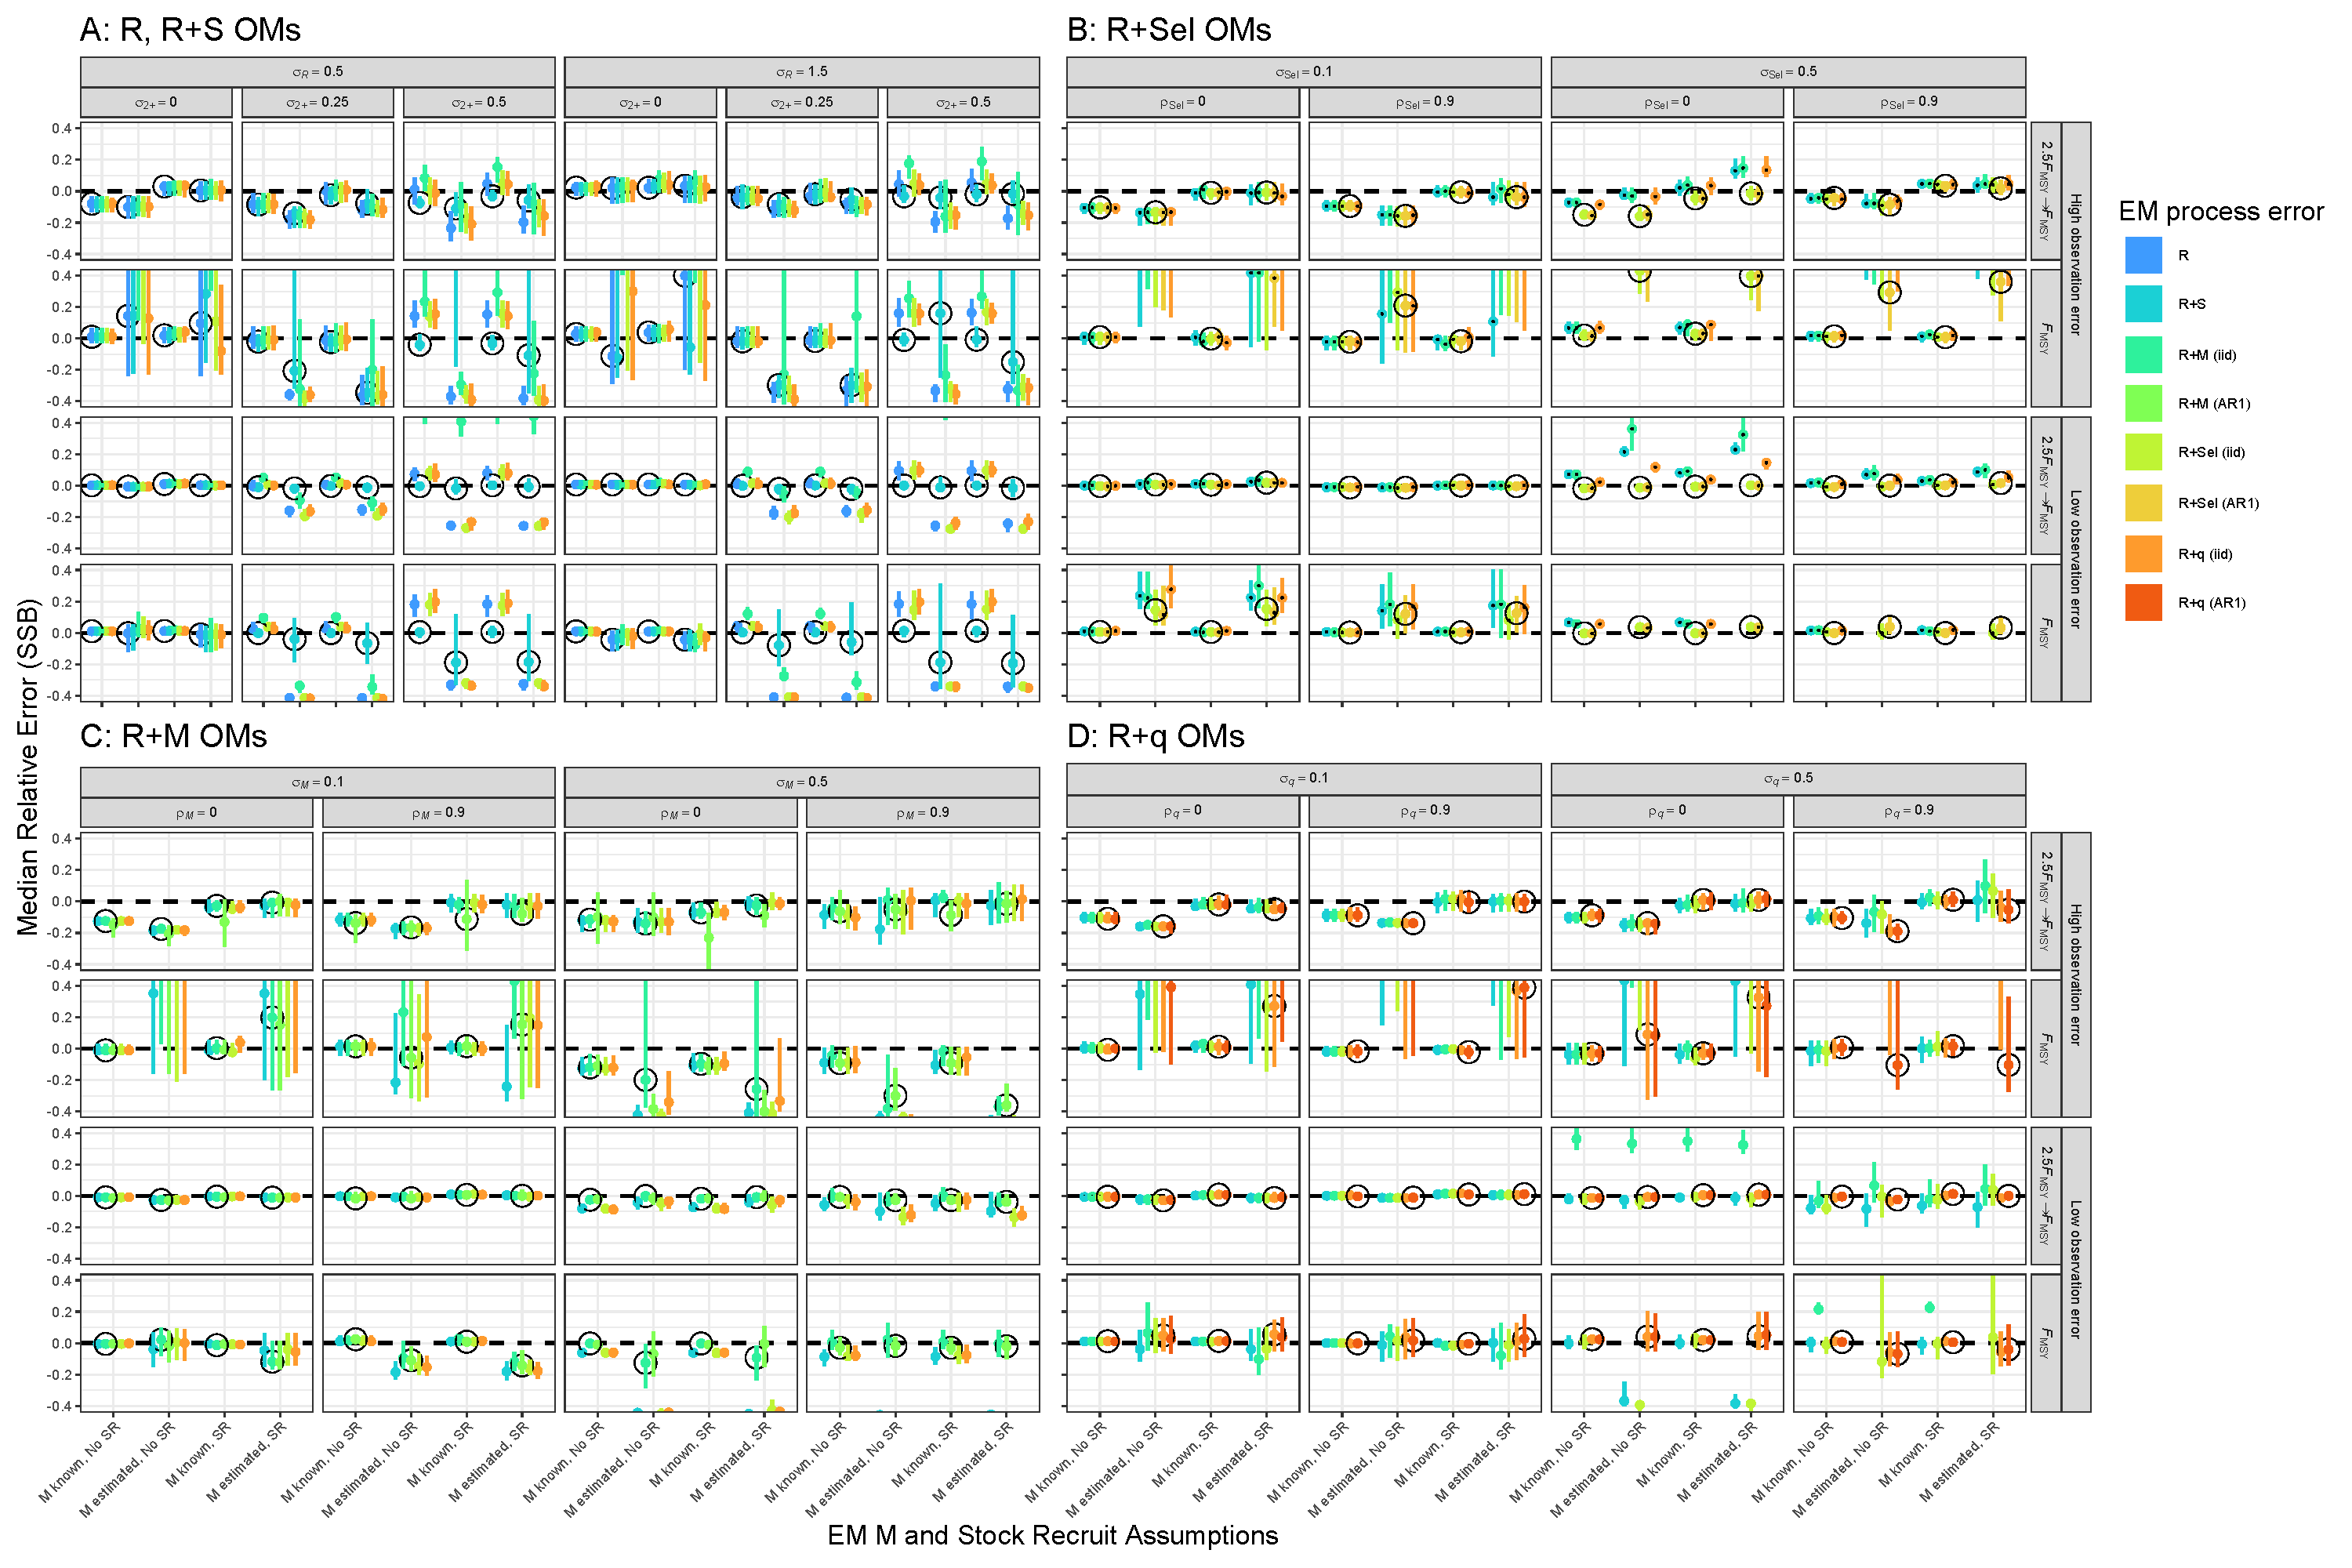
\includegraphics[width = 1.4\textwidth]{term_SSB_bias_plots}
\end{center}
\caption{Median relative error of terminal year SSB for EMs fitted to data sets simulated with alternative process error sources: R and R+S (A), R+Sel (B), R+M (C), or R+q (D). Circled values indicate results where the EM process error structure matches that of the OM and vertical lines represent 95\% confidence intervals.}\label{SSB_rel_error}
\end{figure}
\end{landscape}

\begin{landscape}
\begin{figure}
\begin{center}
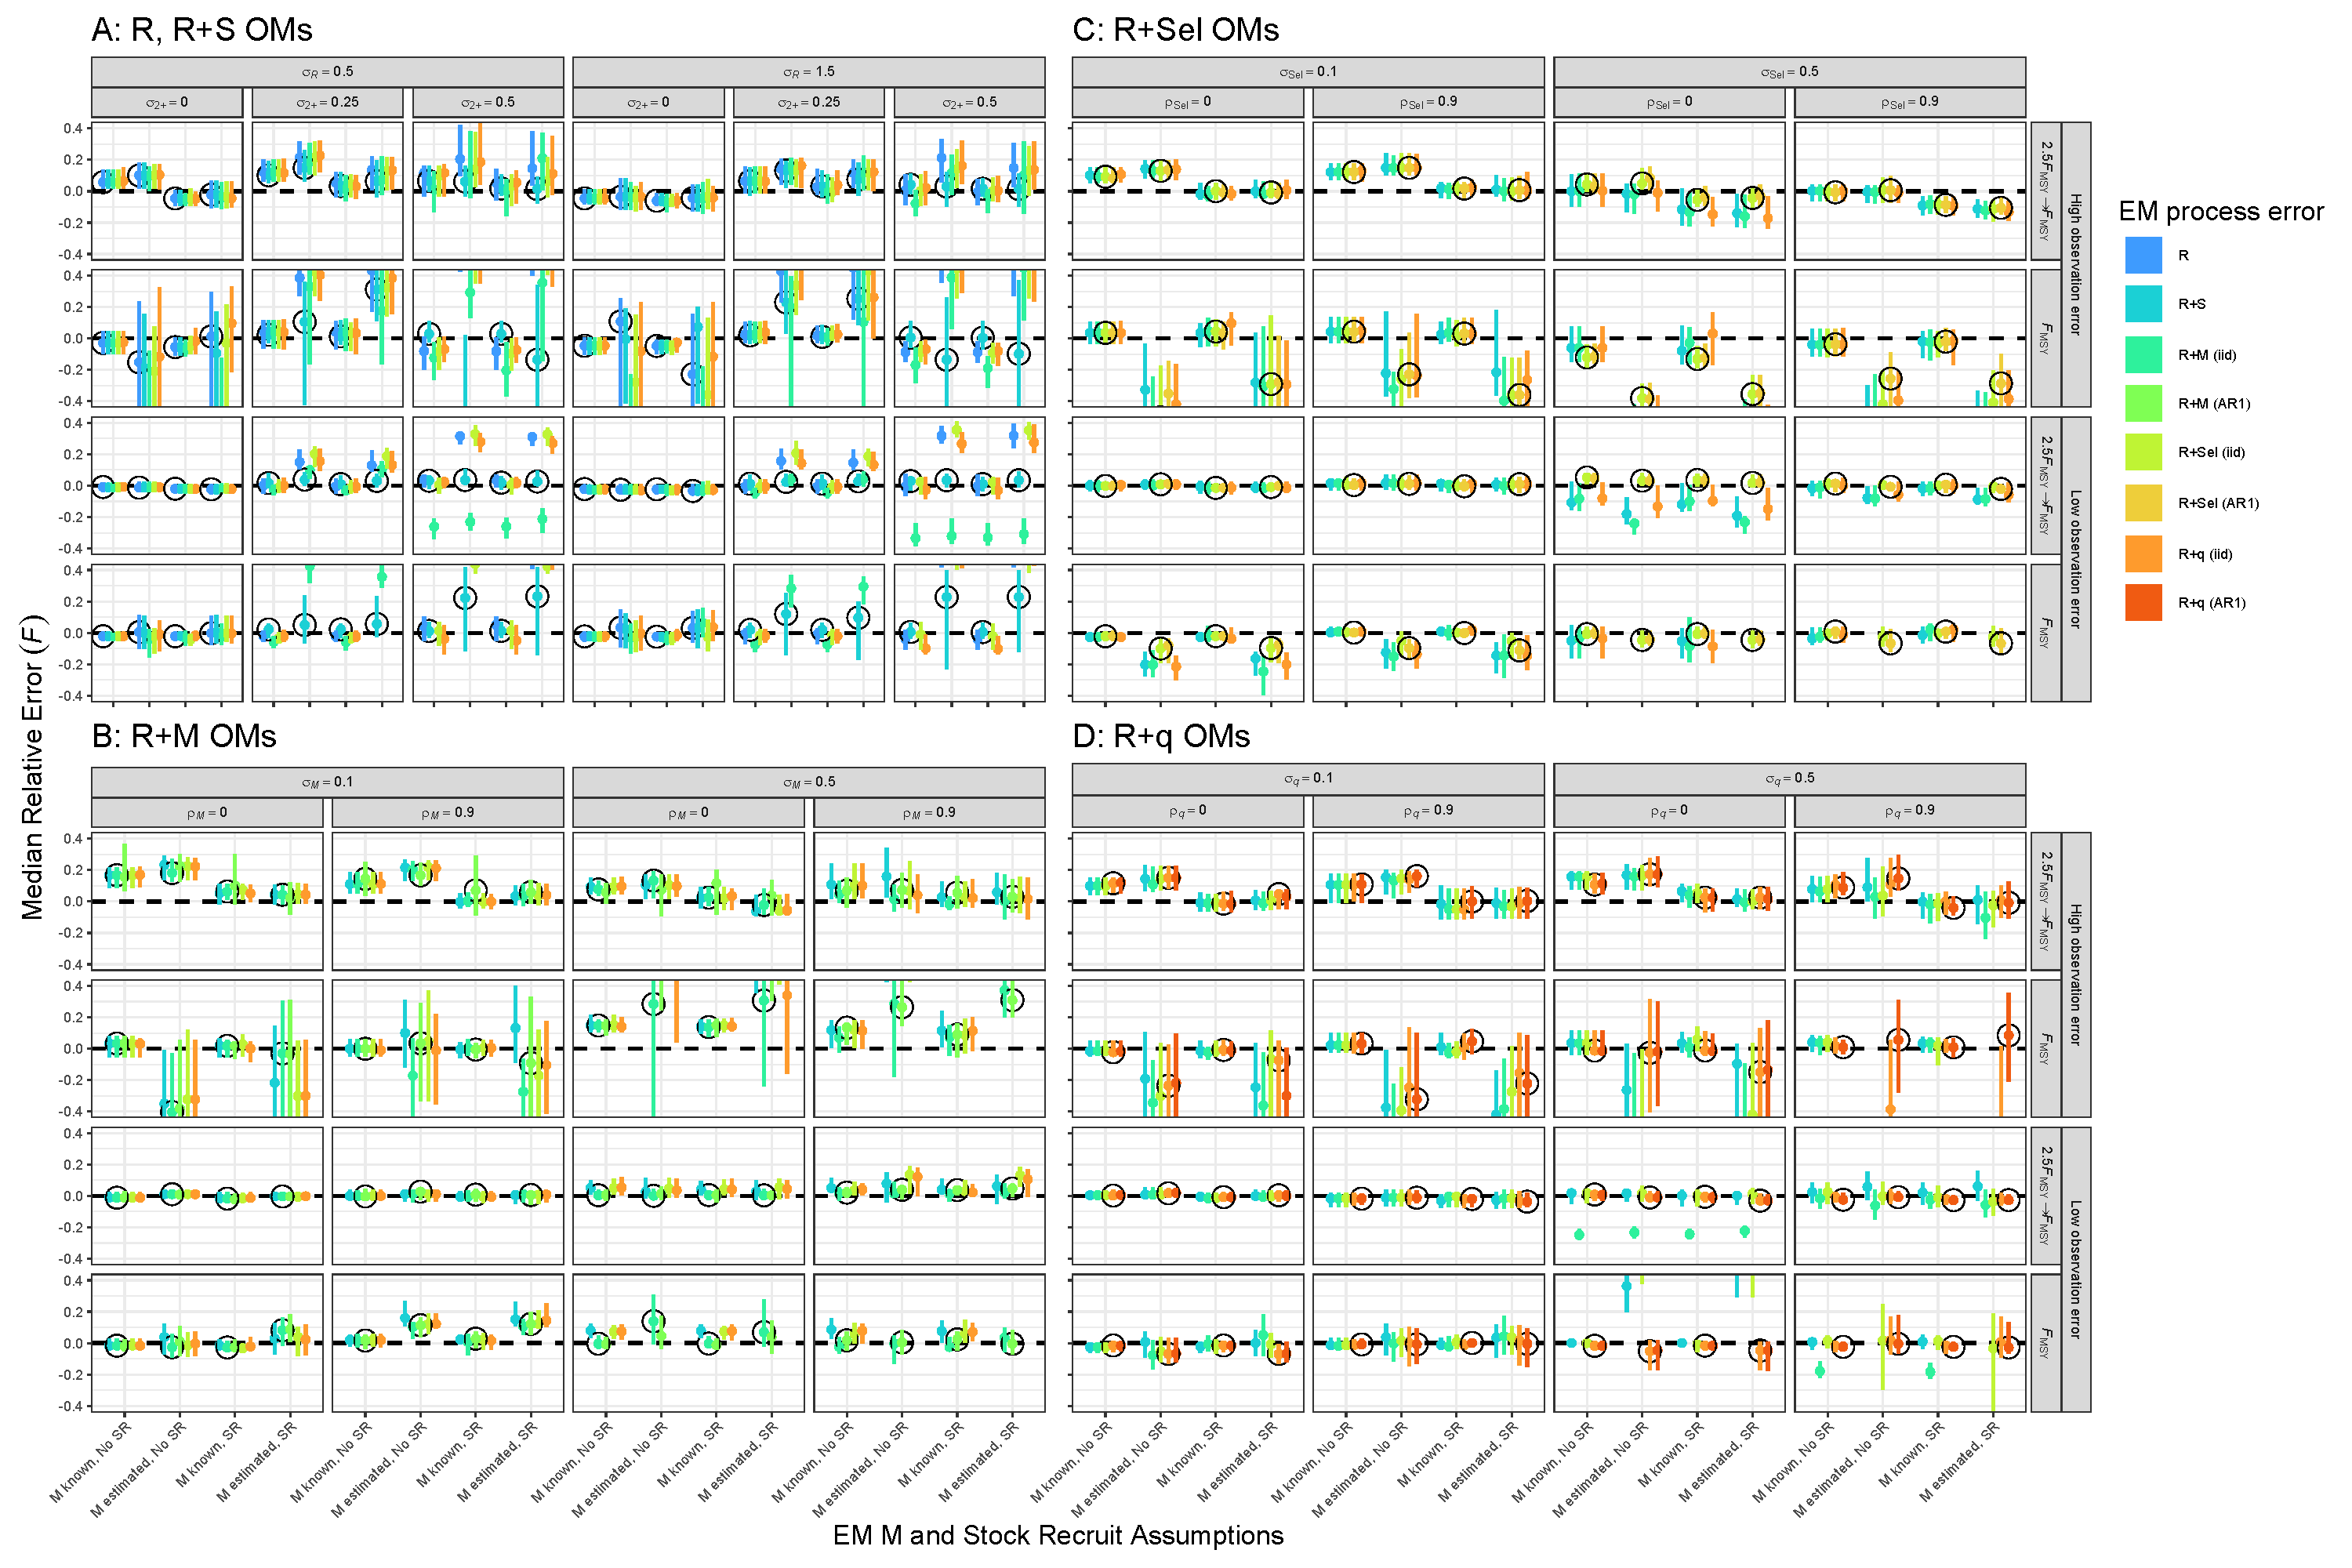
\includegraphics[width = 1.4\textwidth]{term_F_bias_plots}
\end{center}
\caption{Median relative error of terminal year fully-selected fishing mortality for EMs fitted to data sets simulated with alternative process error sources: R and R+S (A), R+Sel (B), R+M (C), or R+q (D). Circled values indicate results where the EM process error structure matches that of the OM and vertical lines represent 95\% confidence intervals.}\label{F_rel_error}
\end{figure}
\end{landscape}

\begin{landscape}
\begin{figure}
\begin{center}
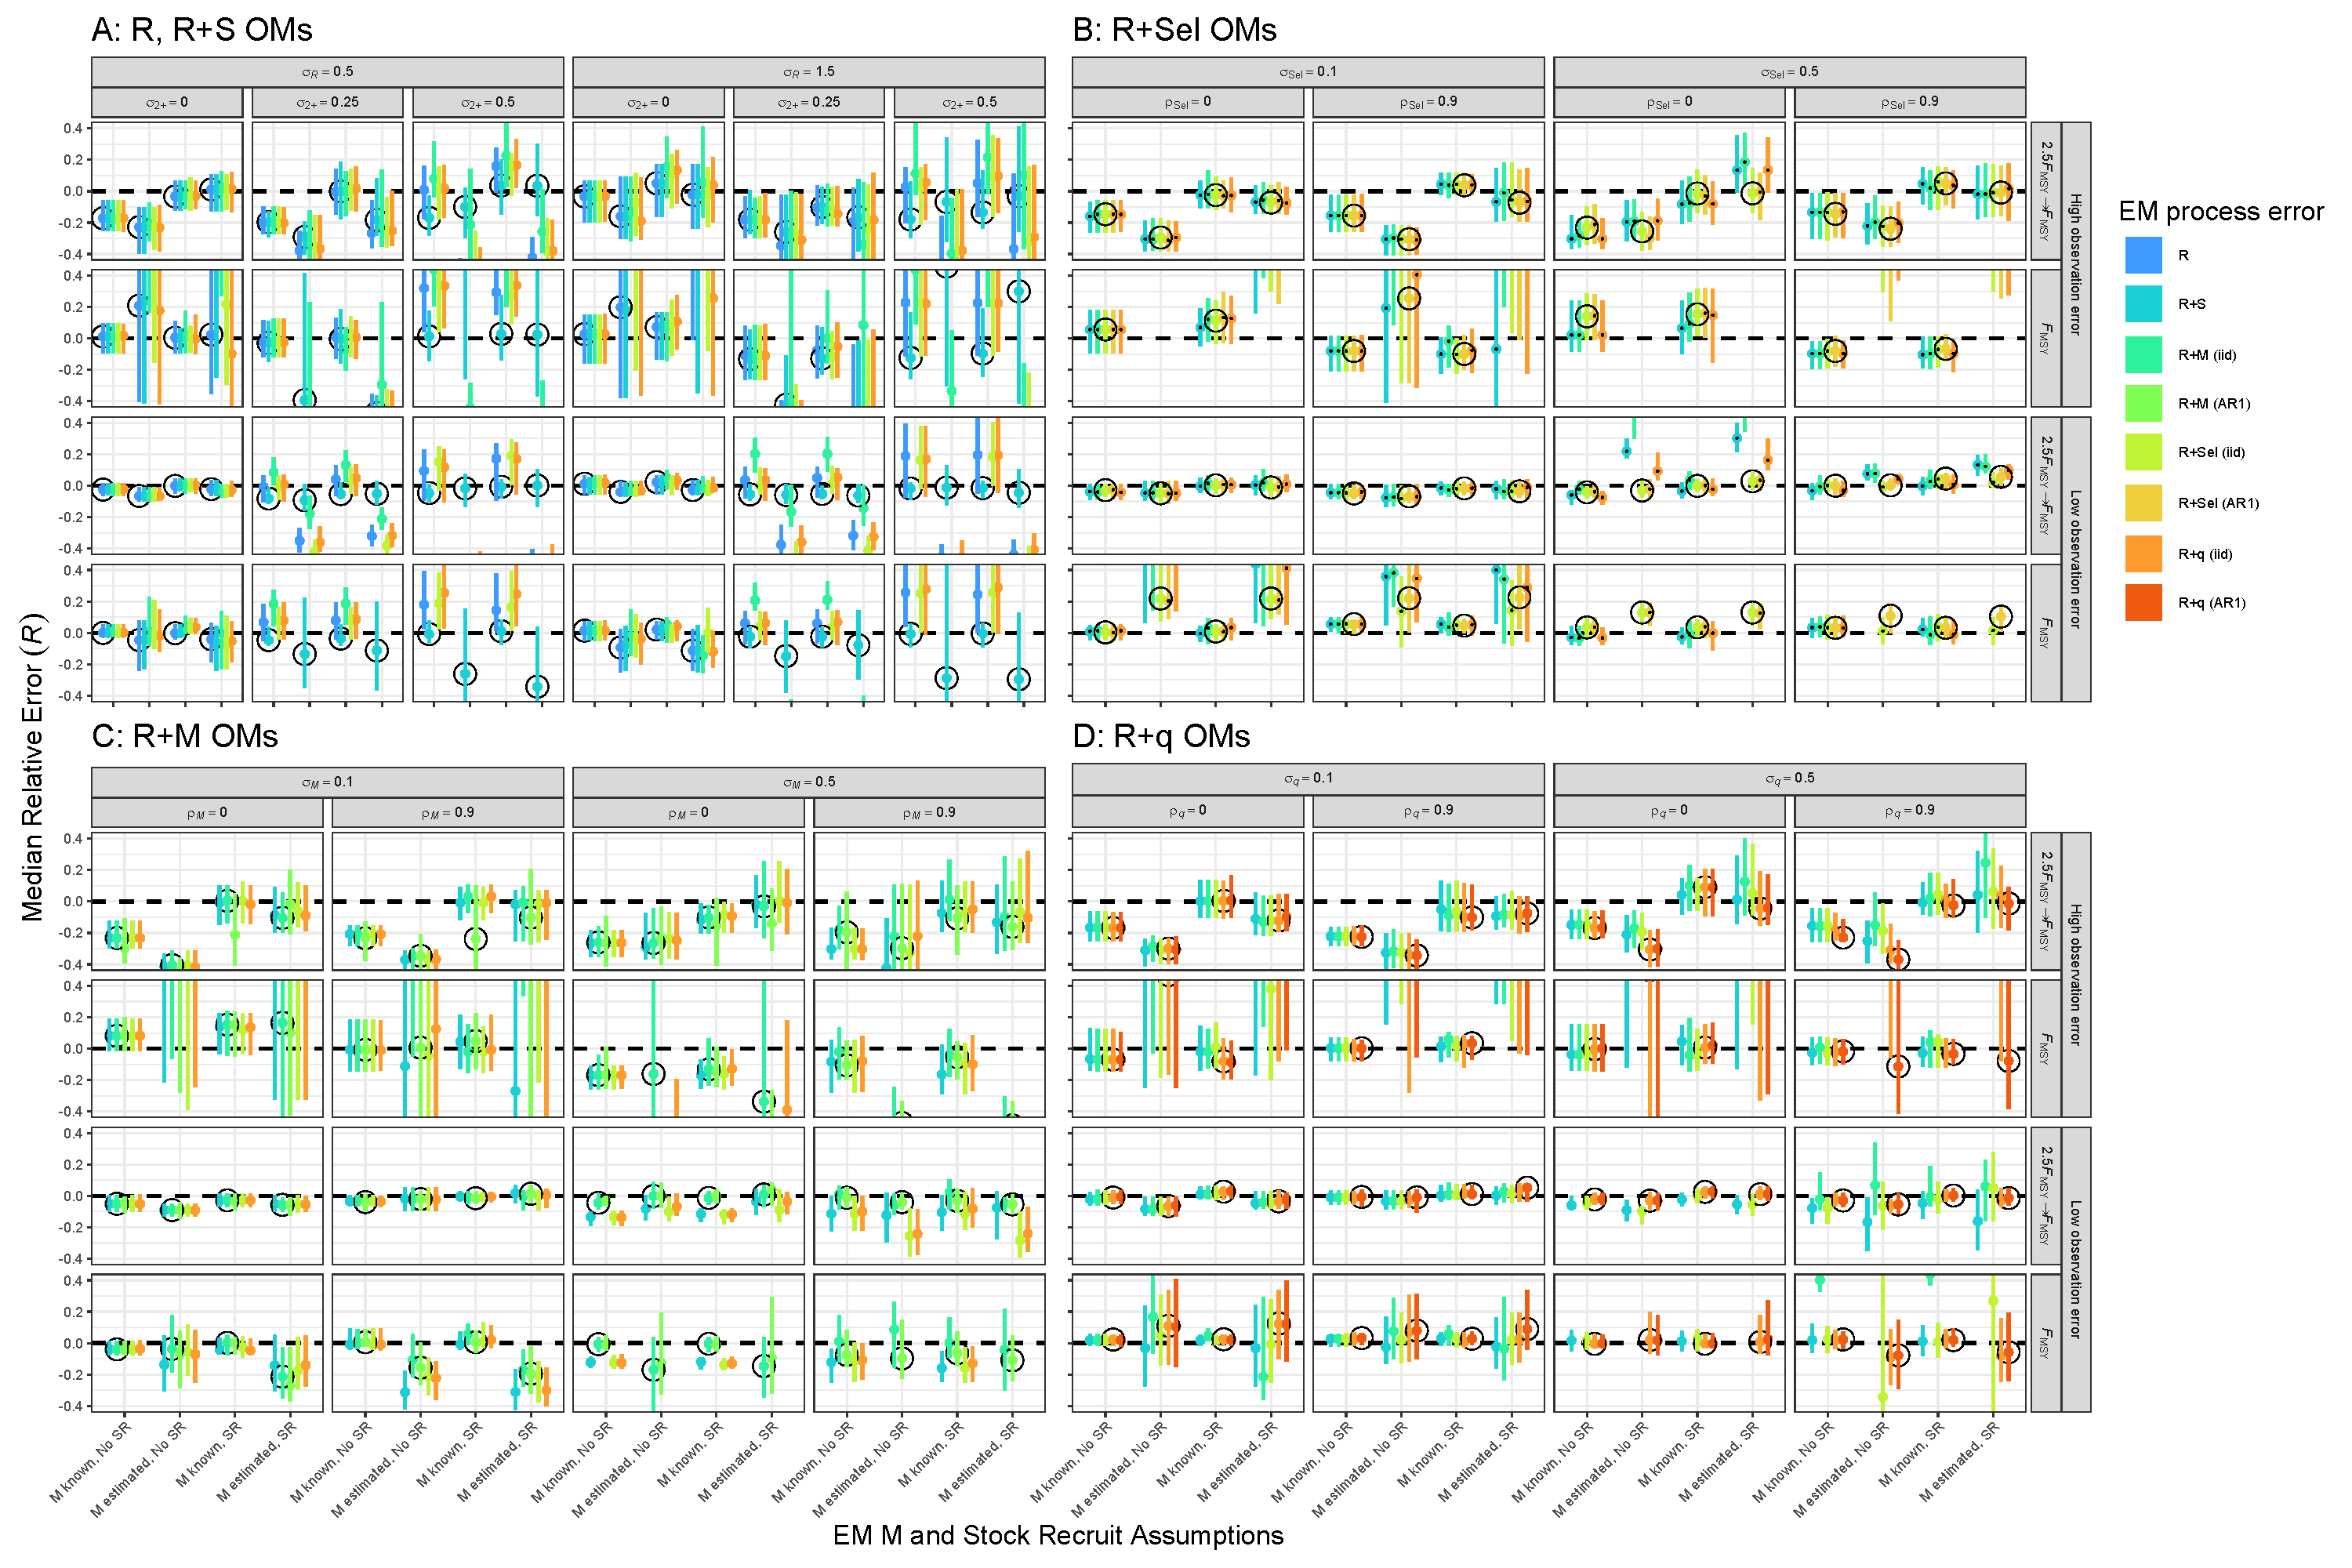
\includegraphics[width = 1.4\textwidth]{term_R_bias_plots}
\end{center}
\caption{Median relative error of terminal year recruitment for EMs fitted to data sets simulated with alternative process error sources: R and R+S (A), R+Sel (B), R+M (C), or R+q (D). Circled values indicate results where the EM process error structure matches that of the OM and vertical lines represent 95\% confidence intervals.}\label{R_rel_error}
\end{figure}
\end{landscape}

\begin{landscape}
\begin{figure}
\begin{center}
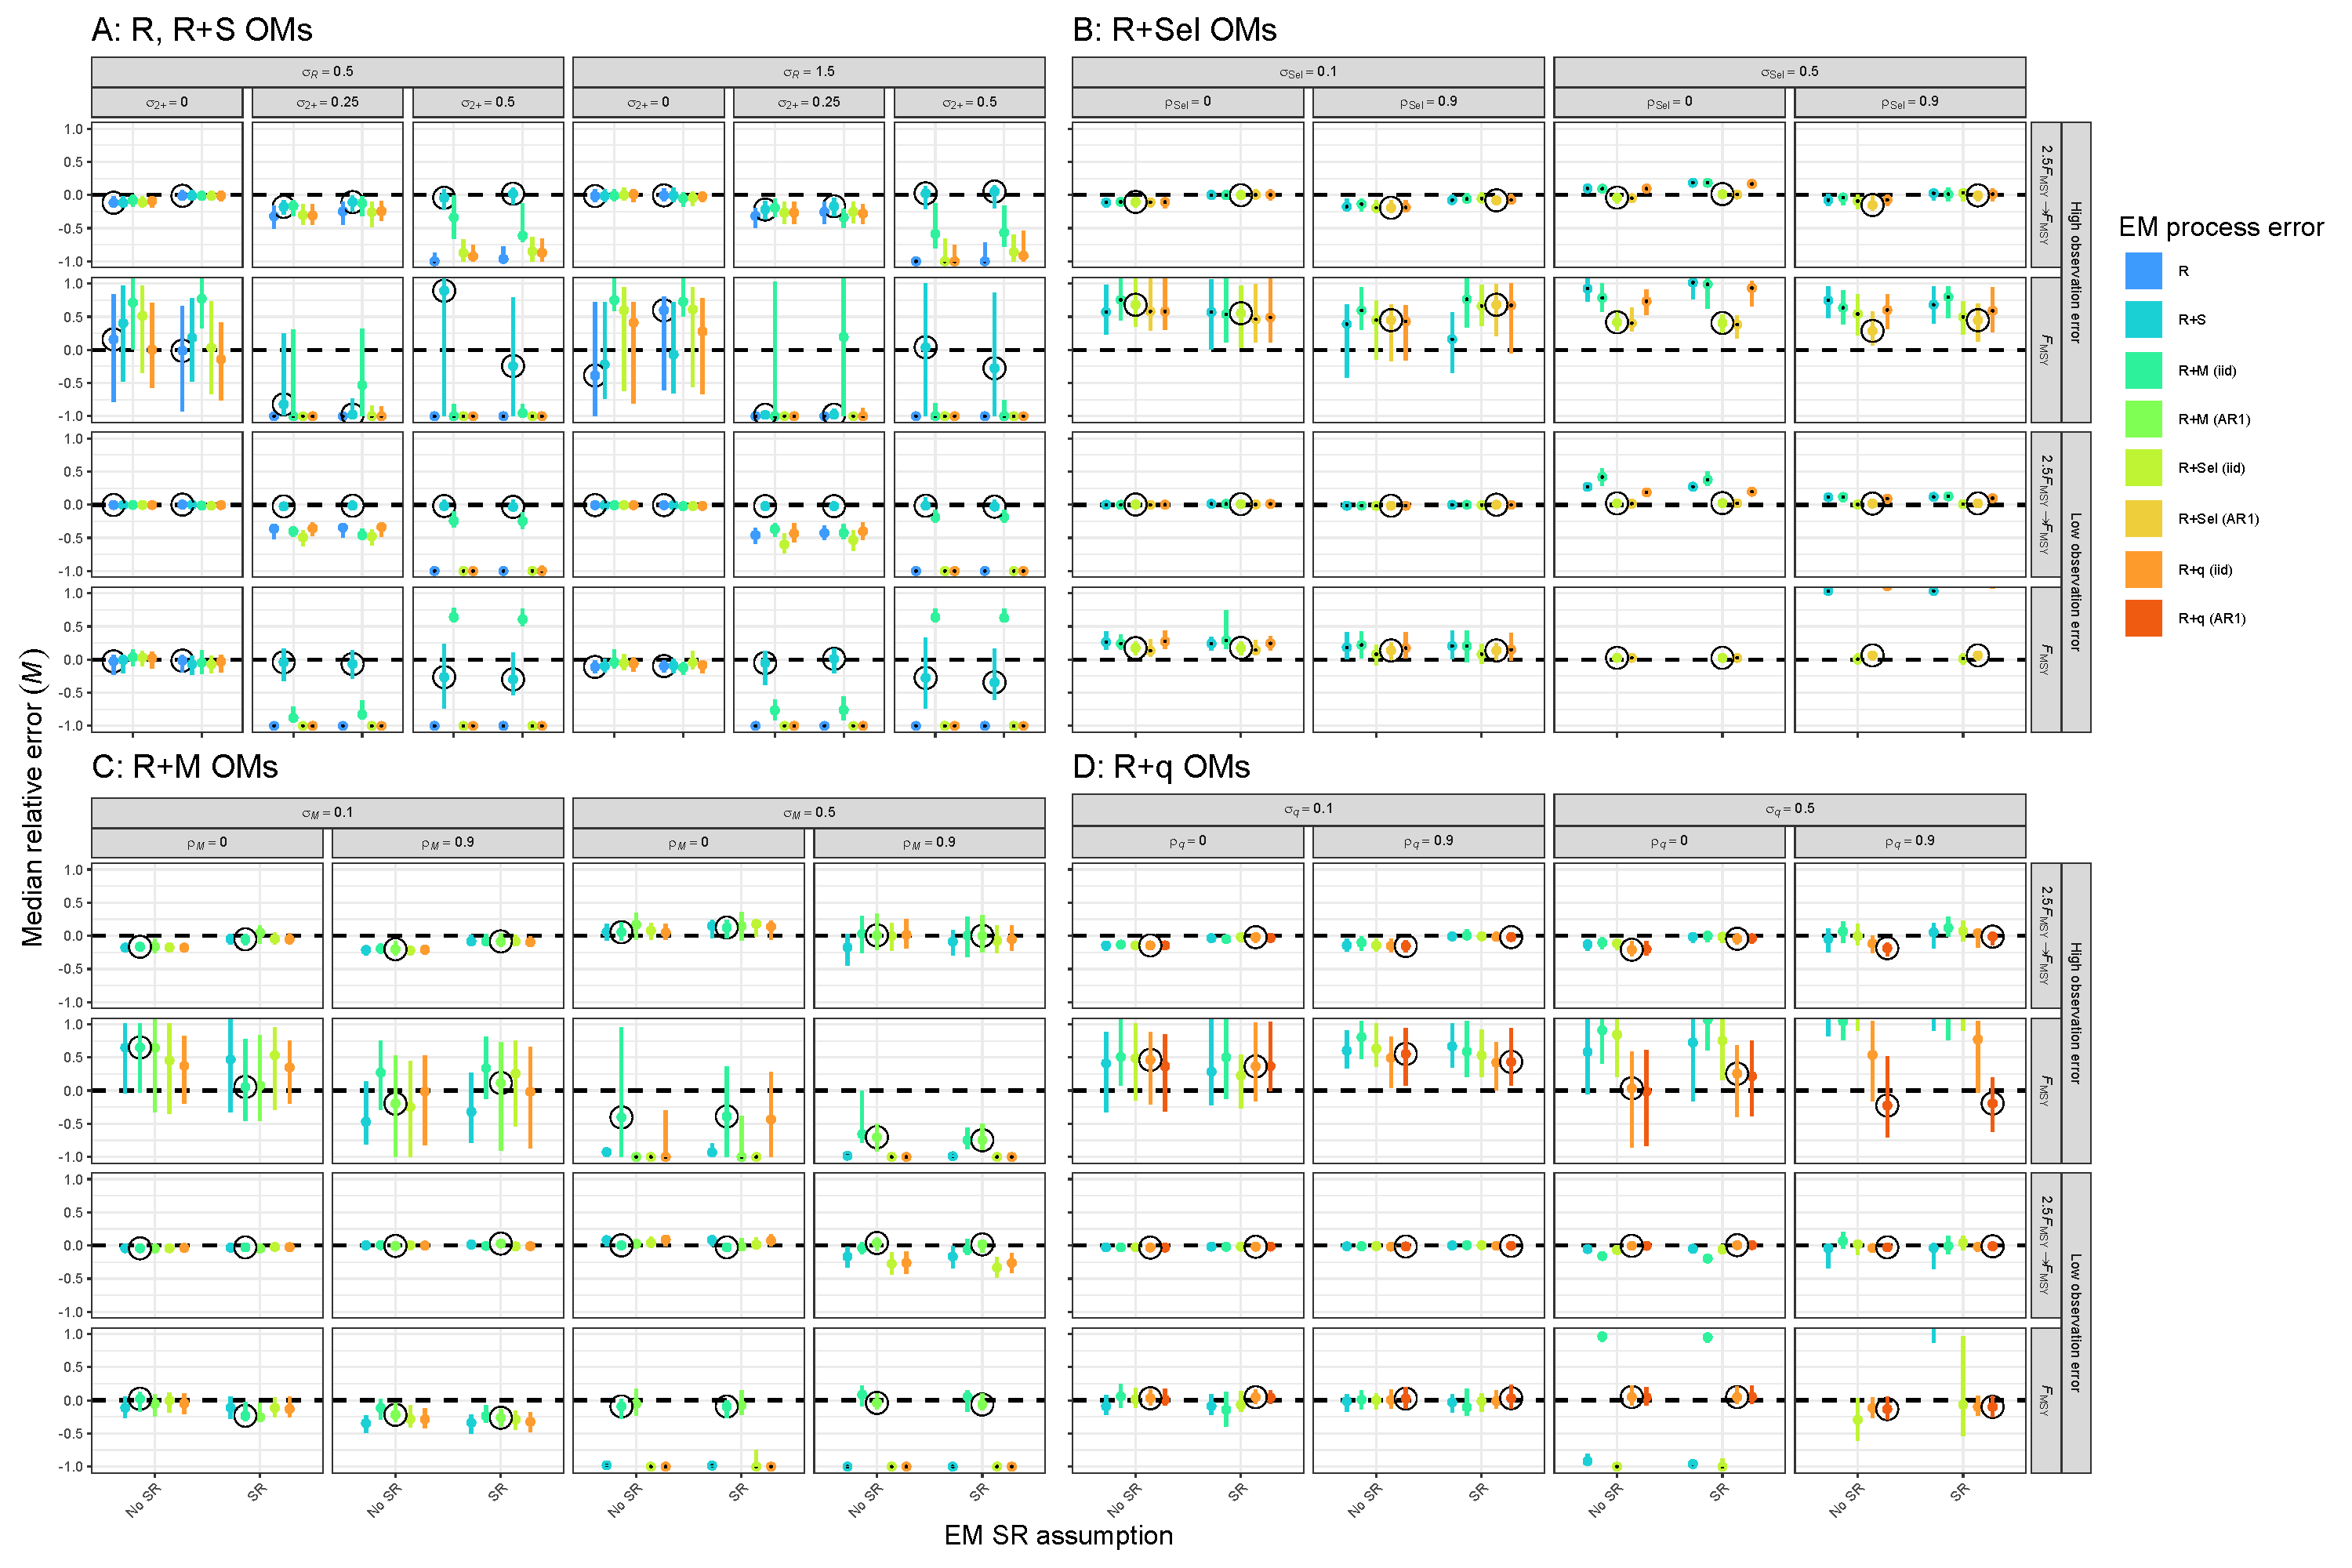
\includegraphics[width = 1.4\textwidth]{M_bias_plots}
\end{center}
\caption{Median relative error of median natural mortality rate for EMs fitted to data sets simulated with alternative process error sources: R and R+S (A), R+Sel (B), R+M (C), or R+q (D). Circled values indicate results where the EM process error structure matches that of the OM and vertical lines represent 95\% confidence intervals.}\label{M_rel_error}
\end{figure}
\end{landscape}

\begin{landscape}
\begin{figure}
\begin{center}
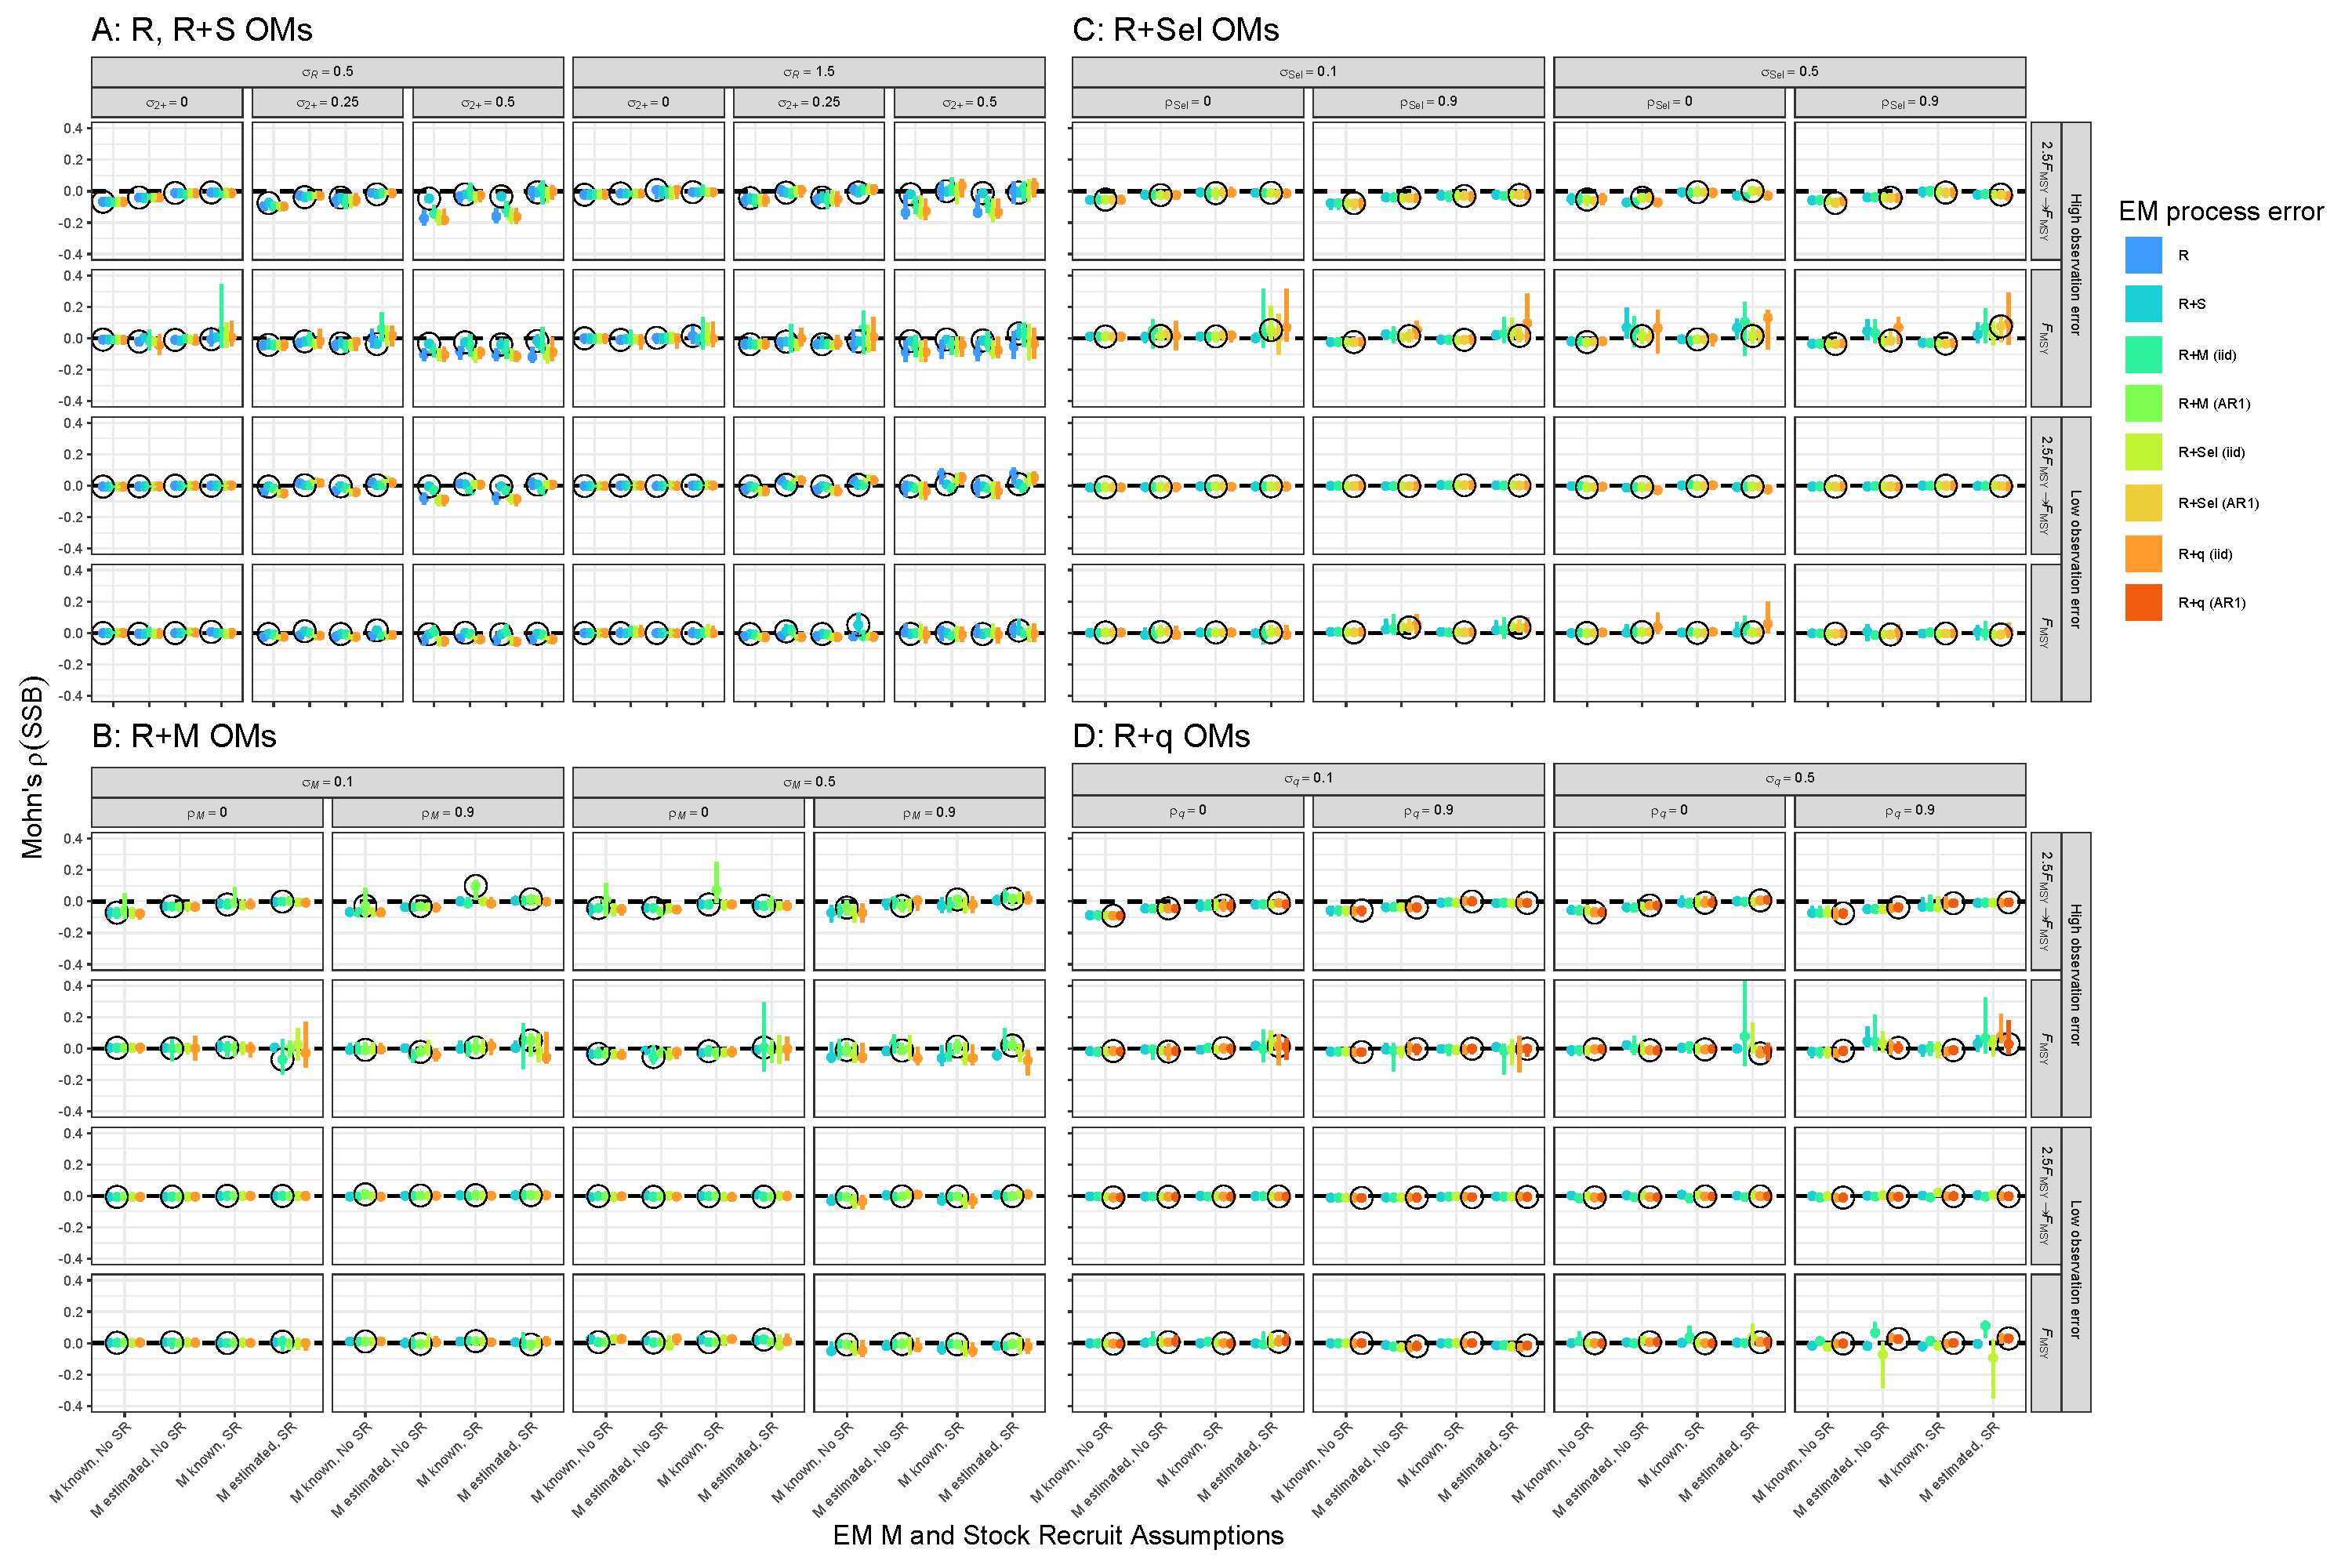
\includegraphics[width = 1.4\textwidth]{mohns_rho_ssb_plots}
\end{center}
\caption{Median Mohn's $\rho$ for SSB for EMs fitted to data sets simulated with alternative process error sources: R and R+S (A), R+Sel (B), R+M (C), or R+q (D). Circled values indicate results where the EM process error structure matches that of the OM and vertical lines represent 95\% confidence intervals.}\label{mohns_rho_ssb}
\end{figure}
\end{landscape}

\begin{landscape}
\begin{figure}
\begin{center}
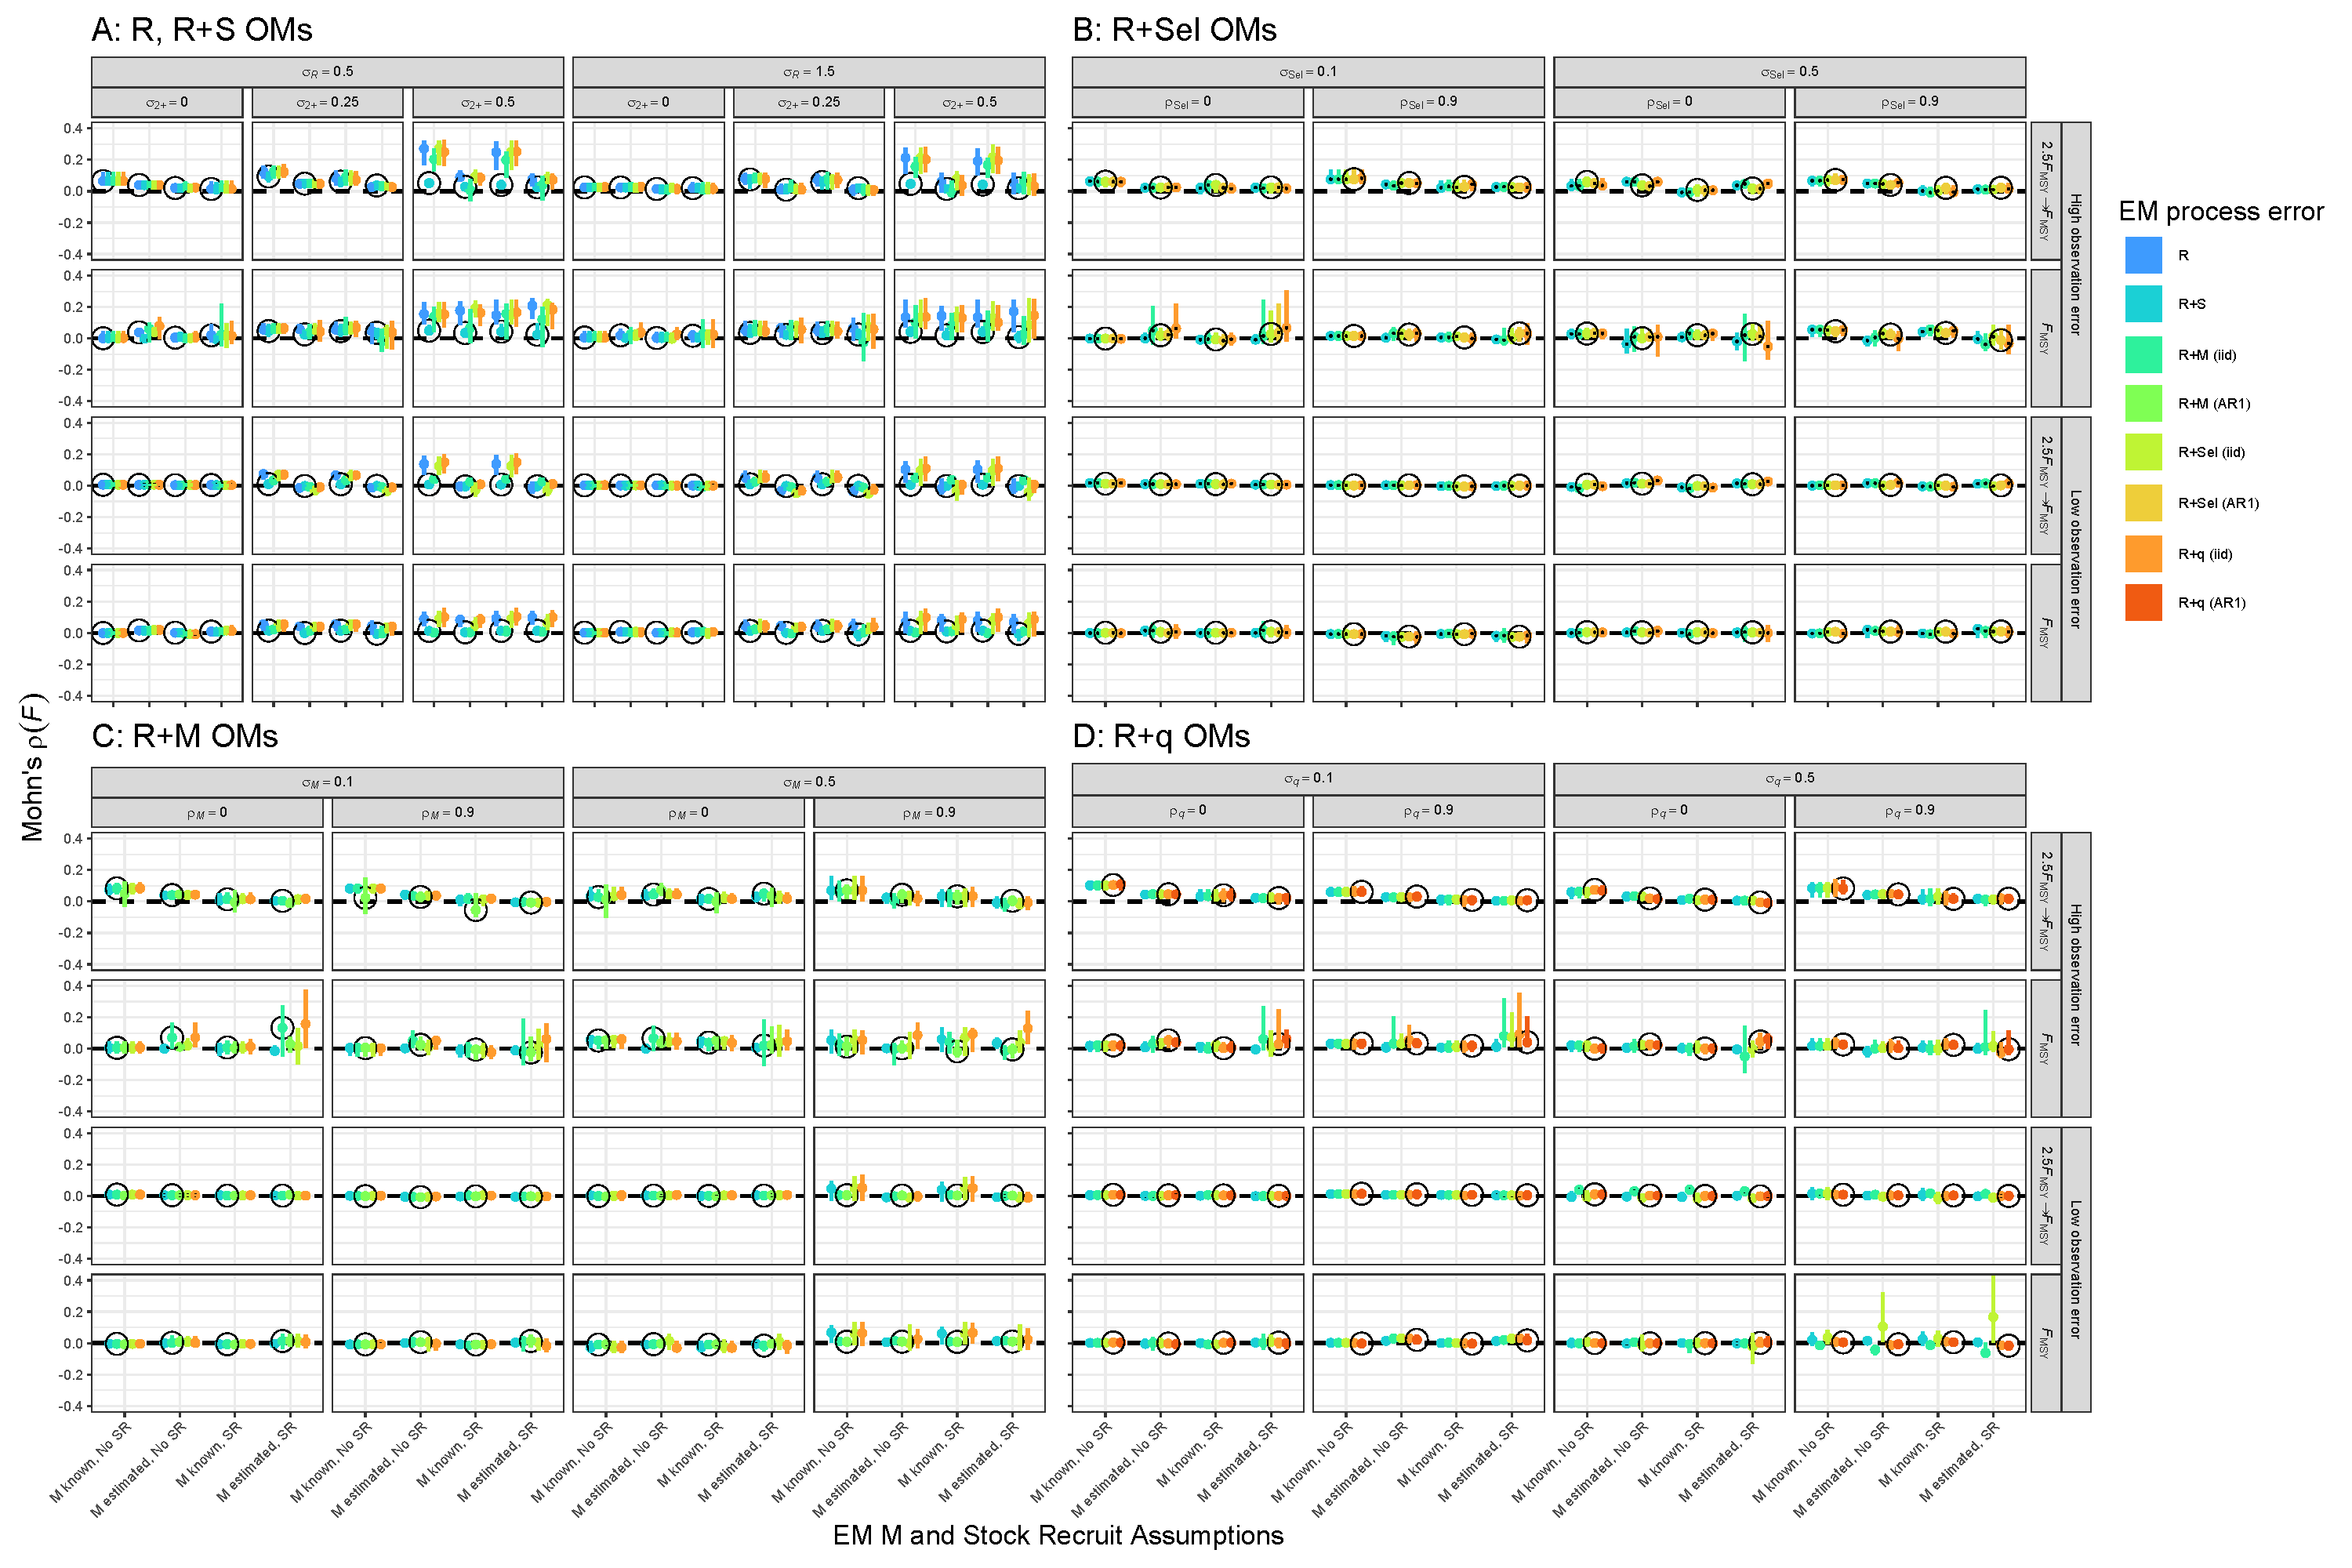
\includegraphics[width = 1.4\textwidth]{mohns_rho_F_plots}
\end{center}
\caption{Median Mohn's $\rho$ of fishing mortality averaged over all age classes for EMs fitted to data sets simulated with alternative process error sources: R and R+S (A), R+Sel (B), R+M (C), or R+q (D). Circled values indicate results where the EM process error structure matches that of the OM and vertical lines represent 95\% confidence intervals.}\label{mohns_rho_F}
\end{figure}
\end{landscape}

\begin{landscape}
\begin{figure}
\begin{center}
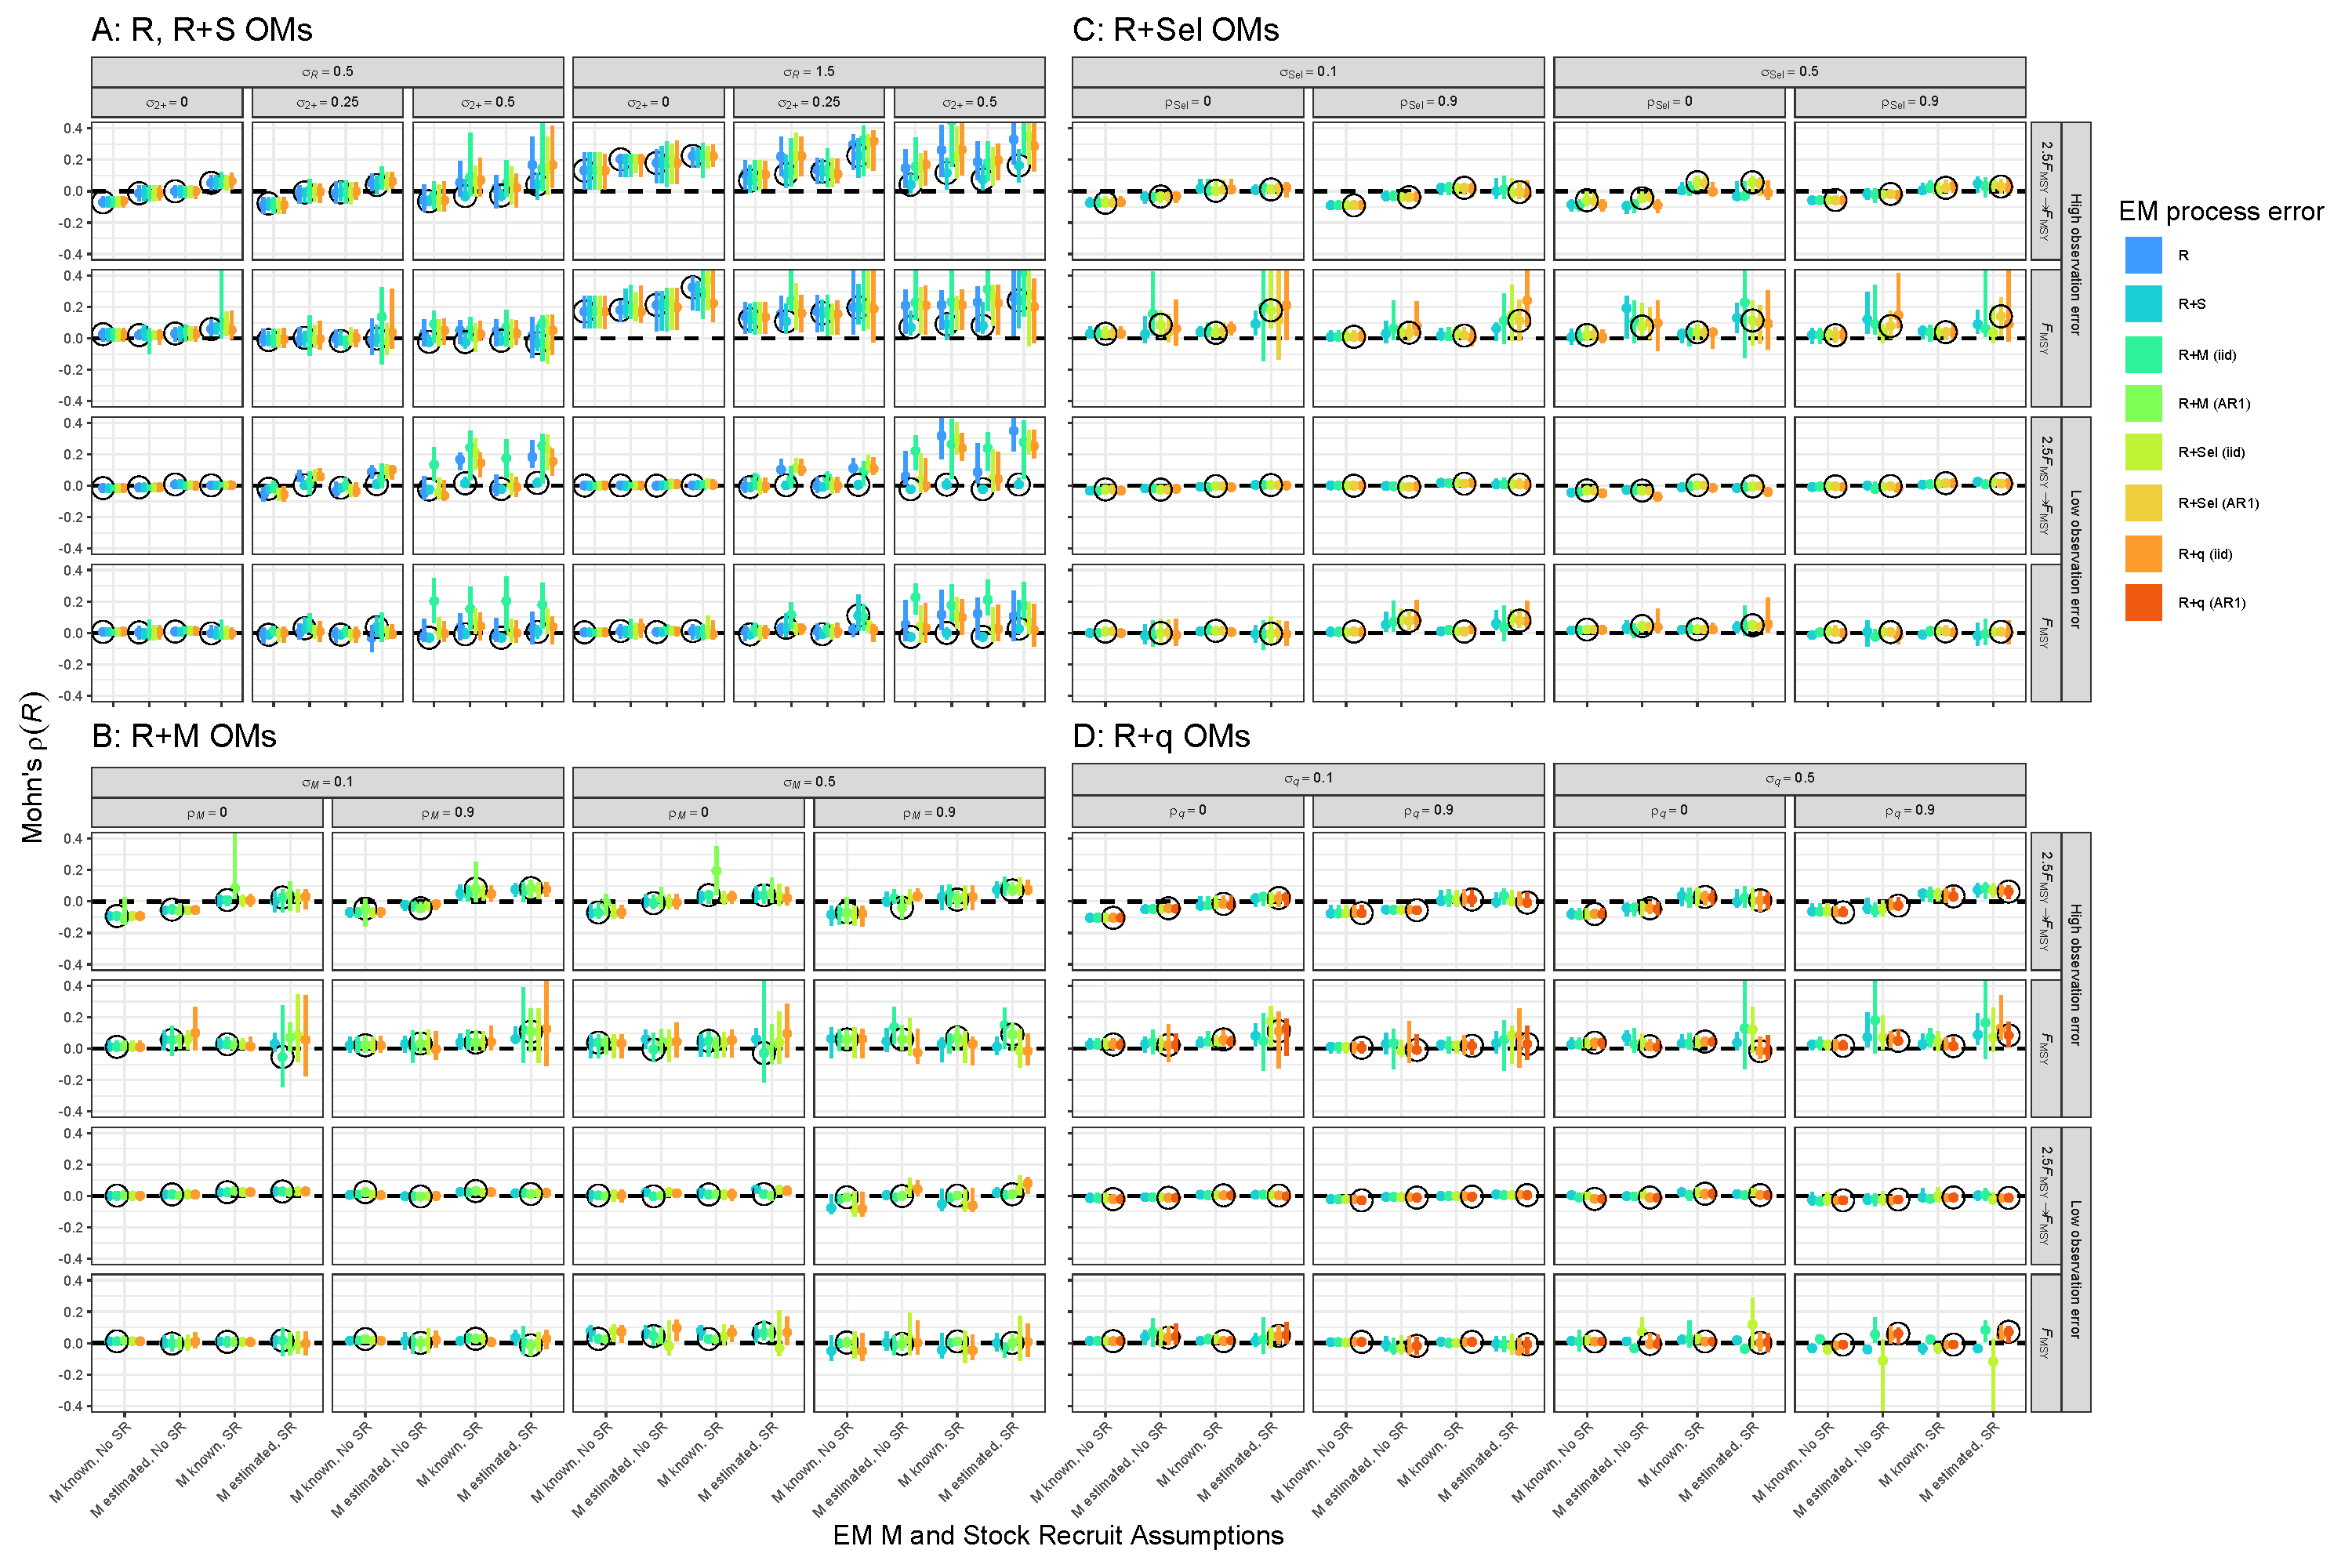
\includegraphics[width = 1.4\textwidth]{mohns_rho_R_plots}
\end{center}
\caption{Median Mohn's $\rho$ of recruitment for EMs fitted to data sets simulated with alternative process error sources: R and R+S (A), R+Sel (B), R+M (C), or R+q (D). Circled values indicate results where the EM process error structure matches that of the OM and vertical lines represent 95\% confidence intervals.}\label{mohns_rho_R}
\end{figure}
\end{landscape}

\begin{landscape}
\begin{figure}
\begin{center}
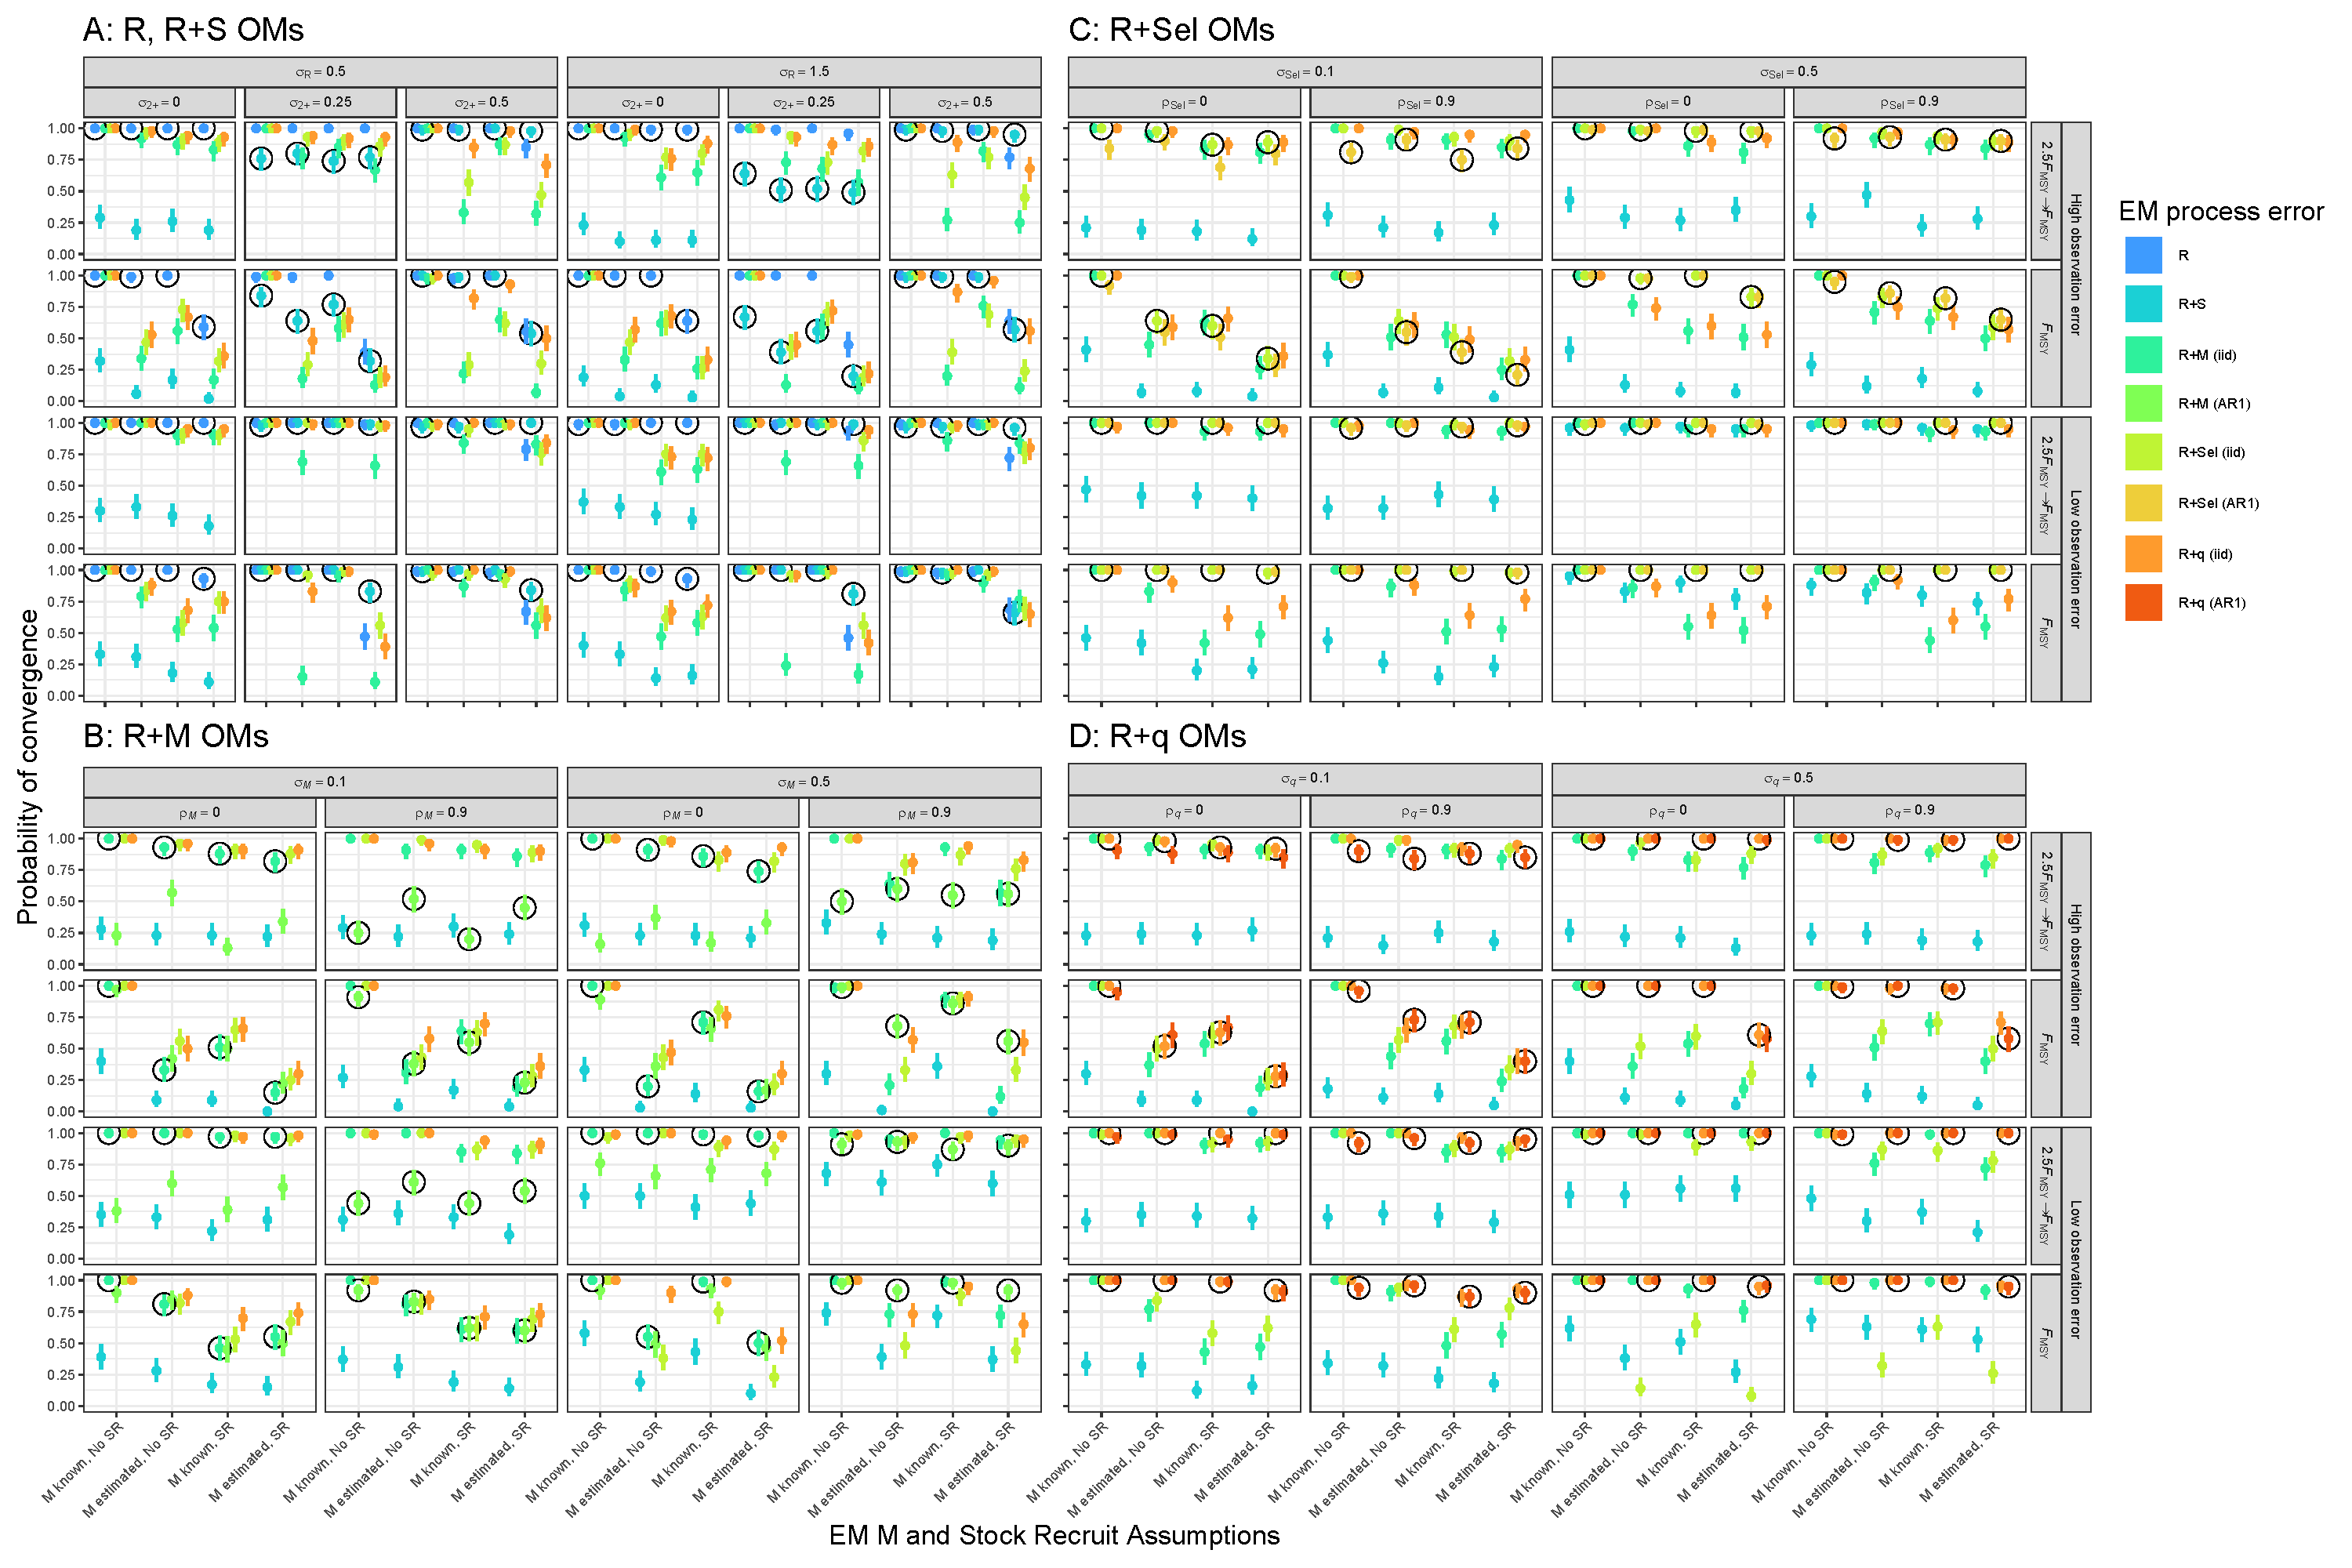
\includegraphics[width = 1.4\textwidth]{type_4_convergence_plots}
\end{center}
\caption{Probability of EMs providing Hessian-based standard errors with alternative process error (colored points and lines), and median natural mortality rate (estimated or known) and Beverton-Holt SRR (estimated or not; along x-axis) assumptions when fitted to OMs that have R and R+S (A), R+Sel (B), R+M (C), or R+q (D) process error sources. Circled values indicate results where the EM process error structure matches that of the OM and vertical lines represent 95\% confidence intervals.}\label{hessian_SE_convergence}
\end{figure}
\end{landscape}

\begin{landscape}
\begin{figure}
\begin{center}
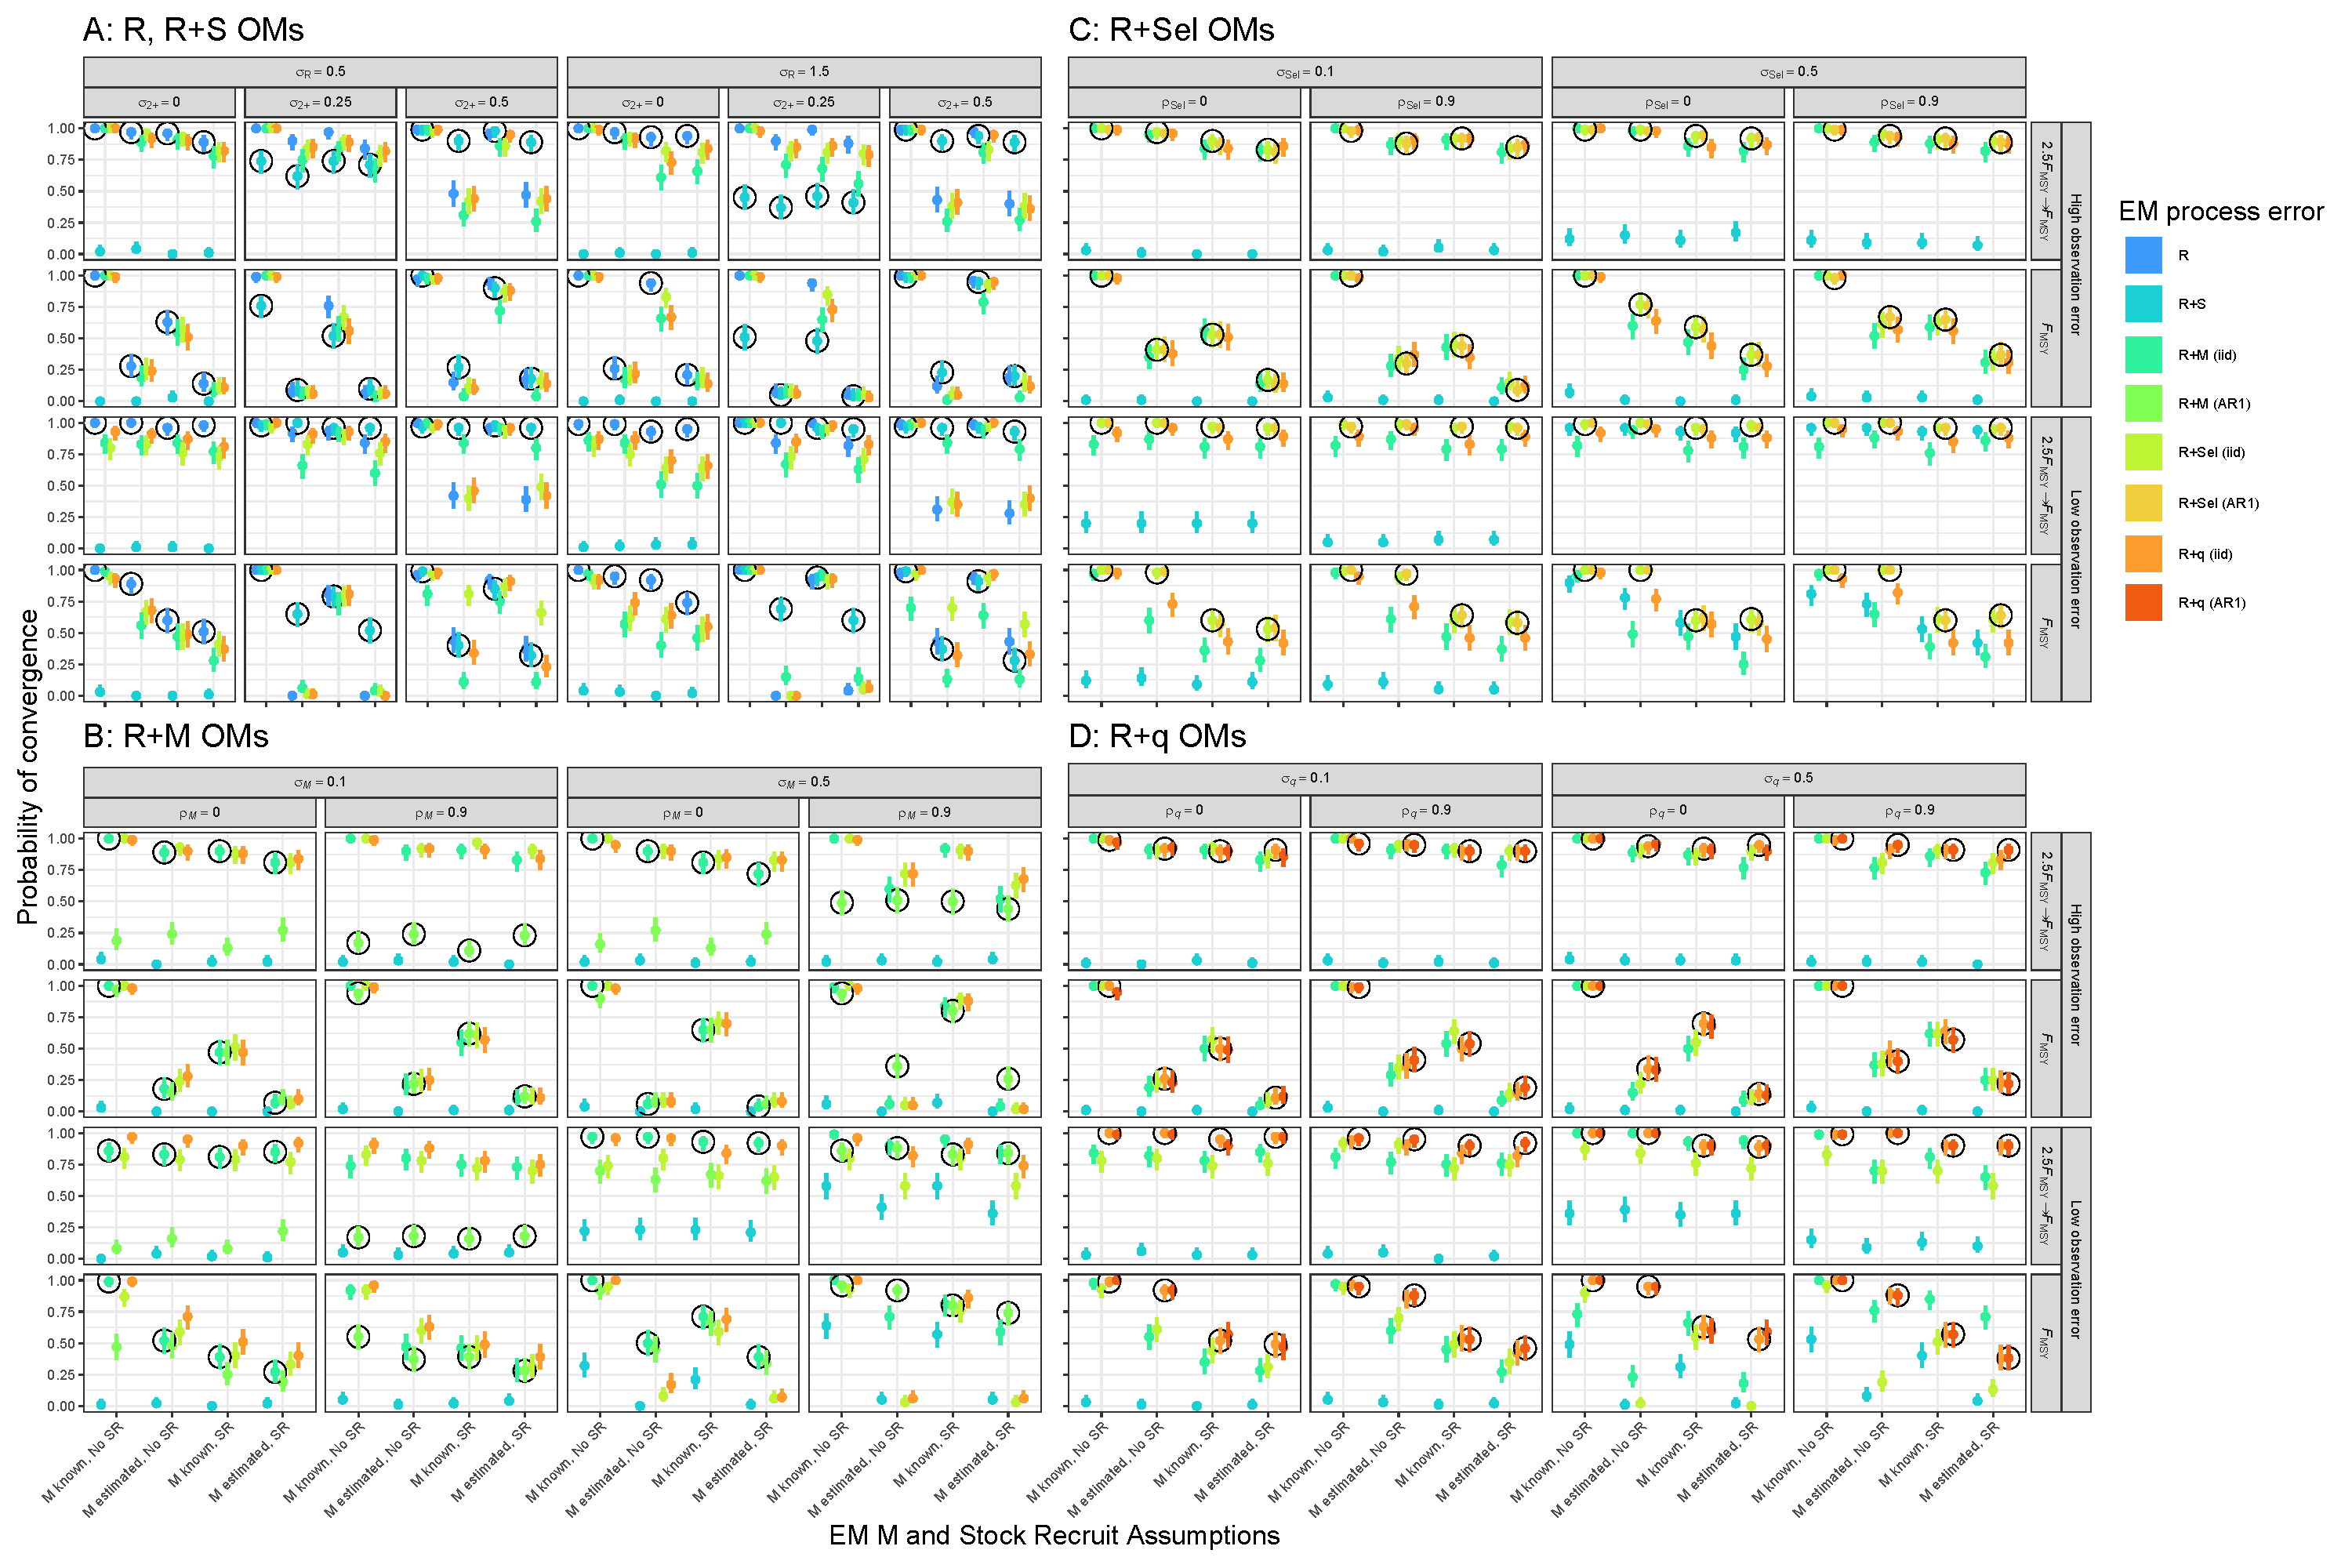
\includegraphics[width = 1.4\textwidth]{type_3_convergence_plots}
\end{center}
\caption{Probability of EMs providing maximum absolute values of gradients less than $10^{-6}$ with alternative process error (colored points and lines), and median natural mortality rate (estimated or known) and Beverton-Holt SRR (estimated or not; along x-axis) assumptions when fitted to OMs that have R and R+S (A), R+Sel (B), R+M (C), or R+q (D) process error sources. Circled values indicate results where the EM process error structure matches that of the OM and vertical lines represent 95\% confidence intervals.}\label{gradient_convergence}
\end{figure}
\end{landscape}

\begin{landscape}
\begin{figure}
\begin{center}
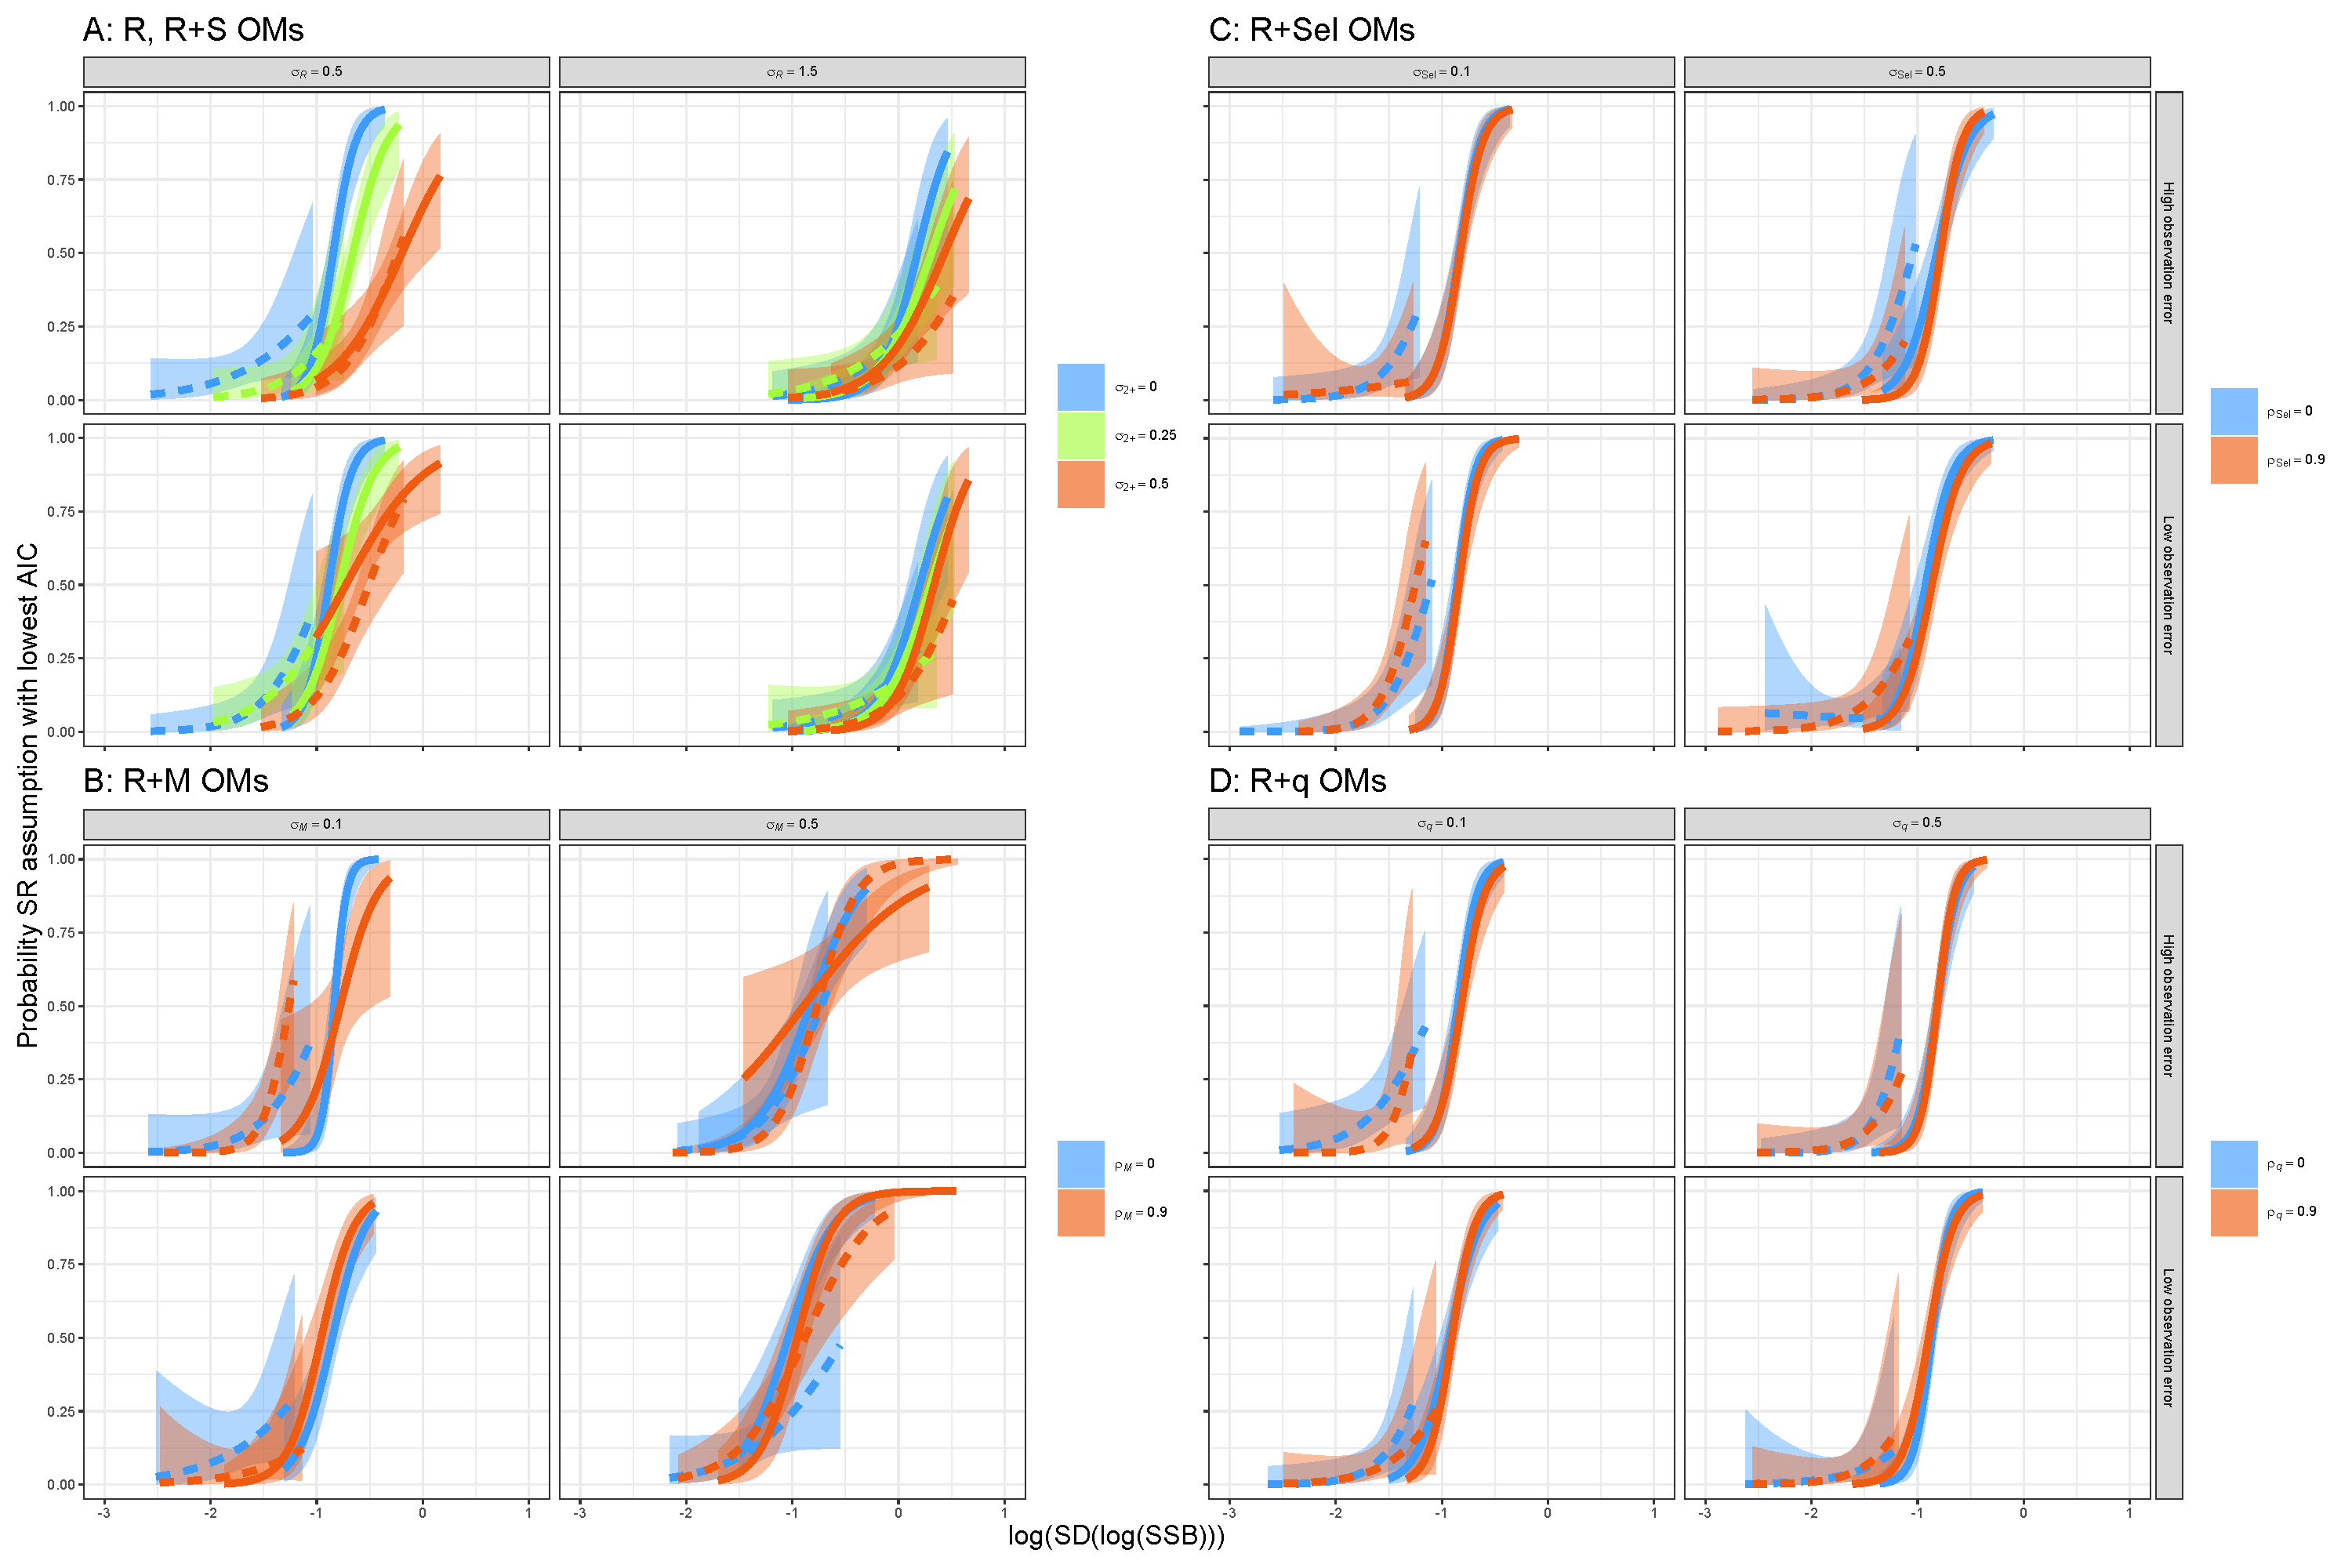
\includegraphics[height = 0.8\textheight]{sr_aic_plots_rev}
\end{center}
\caption{Probability of lowest AIC from logistic regression on the log-standard deviation of the true log(SSB) in each simulation for EM with Beverton-Holt SRRs, rather than the otherwise equivalent EM without the SRR. Results are conditional on median M is known in the EM and alternative assumptions EMs having the correct process error structure: R and R+S (A), R+Sel (B), R+M (C), or R+q (D), and median M is assumed known in the EM. Solid and dashed lines are for OMs with and without temporal contrast in fishing pressure, respectively, and polygons represent 95\% confidence intervals. Range of results indicates the range of log-standard deviation of log(SSB) for simulations of the particular OM.}\label{sr_aic}
\end{figure}
\end{landscape}

\begin{landscape}
\begin{figure}
\begin{center}
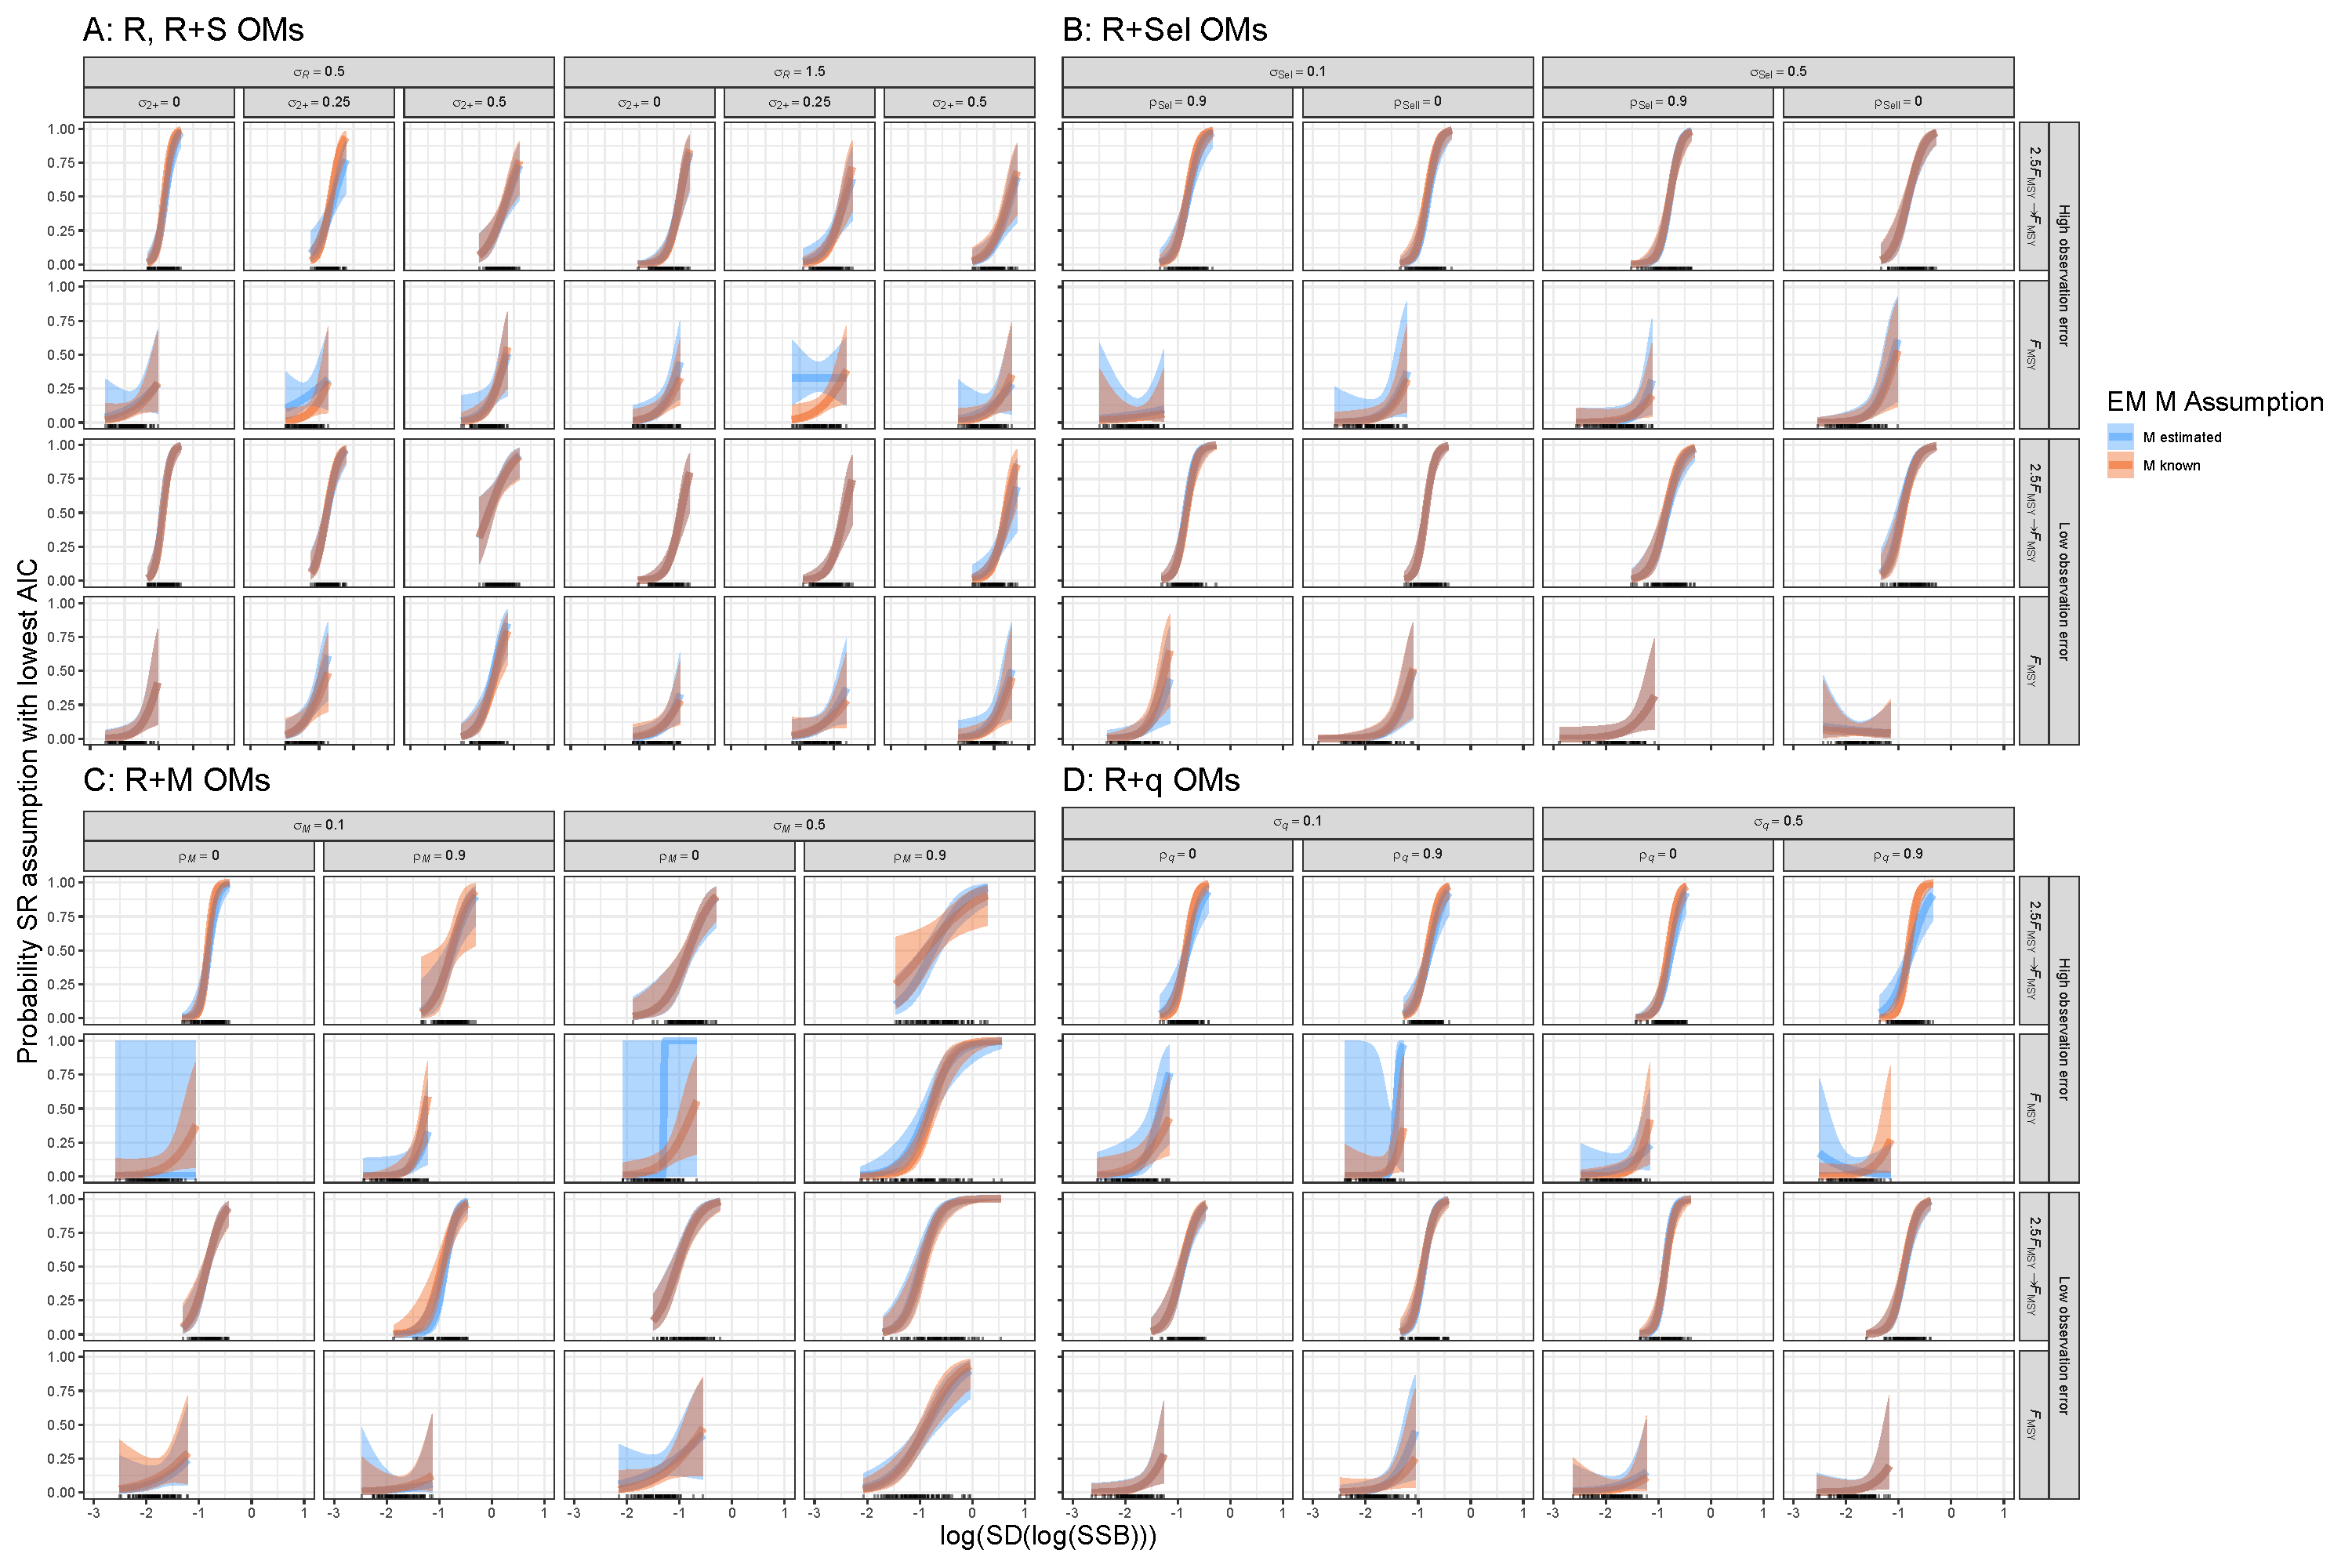
\includegraphics[width = 1.4\textwidth]{sr_aic_plots}
\end{center}
\caption{Estimated probability of lowest AIC from logistic regression on the log-standard deviation of the true log(SSB) in each simulation for EM with Beverton-Holt SRRs, rather than the otherwise equivalent EM without the SRR. Results are conditional on alternative assumptions for median natural mortality rate (estimated or known) and on EMs having the correct process error structure: R and R+S (A), R+Sel (B), R+M (C), or R+q (D). Rug along x-axis denotes $SD(\log(SSB))$ values for each simulation and polygons represent 95\% confidence intervals.}\label{sr_aic_supp}
\end{figure}
\end{landscape}

\begin{table}
\caption{For each OM process error source (columns), percent reduction in deviance for linear regression models fit to transformed Mohn's $\rho$ values for each simulation (Eq. 3) for fishing mortality averaged over all age classes with each OM and EM factor (rows) included individually, combined, and with second and third order interactions.}\label{mohns_rho_F_PRD_table}
{\input{mohns_rho_F_PRD_table}}
\end{table}

\begin{table}
\caption{For each OM process error source (columns), percent reduction in deviance for linear regression models fit to transformed Mohn's $\rho$ values for each simulation (Eq. 3) for recruitment with each OM and EM factor (rows) included individually, combined, and with second and third order interactions.}\label{mohns_rho_R_PRD_table}
{\input{mohns_rho_R_PRD_table}}
\end{table}

\end{document}
